\chapter{重积分}

\section{二重积分的概念}

\subsection{平面图形的面积}

为了研究定义在平面图形 (即平面点集) 上函数的积分, 我们首先讨论平面有界图形的面积问题.

所谓一个平面图形 \(P\) 是有界的,是指构成这个平面图形的点集是平面上的有界点集,即存在一矩形 \(R\) ,使得 \(P \subset  R\) .

设 \(P\) 是一平面有界图形,用某一平行于坐标轴的一组直线网 \(T\) 分割这个图形 (图 21-1). 这时直线网 \(T\) 的网眼——小闭矩形 \({\Delta }_{i}\) 可分为三类: (i) \({\Delta }_{i}\) 上的点都是 \(P\) 的内点,(ii) \({\Delta }_{i}\) 上的点都是 \(P\) 的外点,(iii) \({\Delta }_{i}\) 上含有 \(P\) 的边界点.

\begin{figure}
	\centering
	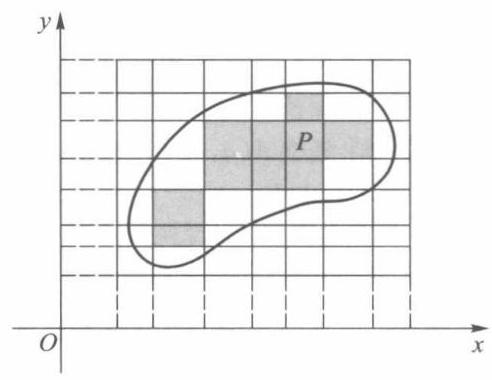
\includegraphics[width=.3\textwidth]{images/P155.jpg}
	\caption{图 $21-1$}
	\label{fig:P155}
\end{figure}

我们将所有属于直线网 \(T\) 的第 (i) 类小矩形 (图 21-1 中阴影部分) 的面积加起来, 记这个和数为 \({s}_{P}\left( T\right)\) ,则有 \({s}_{P}\left( T\right)  \leq  {\Delta }_{R}\) (这里 \({\Delta }_{R}\) 表示包含 \(P\) 的那个矩形 \(R\) 的面积); 将所有第 (i) 类与第 (iii) 类小矩形 (图 21-1 中含有粗线的小矩形) 的面积加起来,记这个和数为 \({S}_{P}\left( T\right)\) ,则有 \({s}_{P}\left( T\right)  \leq  {S}_{P}\left( T\right) .\)

由确界存在定理可以推得,对于平面上所有直线网,数集 \(\left\{  {{s}_{P}\left( T\right) }\right\}\) 有上确界,数集 \(\left\{  {{S}_{P}\left( T\right) }\right\}\) 有下确界,记
\[
{I}_{P} = \mathop{\sup }\limits_{T}\left\{  {{s}_{P}\left( T\right) }\right\}  ,\;{\bar{I}}_{P} = \mathop{\inf }\limits_{T}\left\{  {{S}_{P}\left( T\right) }\right\}  .
\]
显然有
\[
0 \leq  {\underline{I}}_{P} \leq  {\bar{I}}_{P}. \tag{1}
\]
通常称 \({\underline{I}}_{P}\) 为 \(P\) 的内面积, \({\bar{I}}_{P}\) 为 \(P\) 的外面积.

%定义  1
\begin{definition}{}{def:}

\end{definition}
若平面图形 \(P\) 的内面积 \({I}_{P}\) 等于它的外面积 \({\bar{I}}_{P}\) ,则称 \(P\) 为可求面积,并称其共同值 \({I}_{P} = {\underline{I}}_{P} = {\bar{I}}_{P}\) 为 \(P\) 的面积.

%定理 21.1
\begin{theorem}{}{the:}

\end{theorem}
 平面有界图形 \(P\) 可求面积的充要条件是: 对任给的 \(\varepsilon  > 0\) ,总存在直线网 \(T\) ,使得
\[
{S}_{P}\left( T\right)  - {s}_{P}\left( T\right)  < \varepsilon . \tag{2}
\]
%证
\begin{proof}

\end{proof}
[必要性] 设平面有界图形 \(P\) 的面积为 \({I}_{P}\) . 由定义 1,有 \({I}_{P} = {\underline{I}}_{P} = {\bar{I}}_{P}\) . 对任给的 \(\varepsilon  > 0\) ,由 \({I}_{P}\) 及 \({\bar{I}}_{P}\) 的定义知道,分别存在直线网 \({T}_{1}\) 与 \({T}_{2}\) ,使得
\[
{s}_{P}\left( {T}_{1}\right)  > {I}_{P} - \frac{\varepsilon }{2},\;{S}_{P}\left( {T}_{2}\right)  < {I}_{P} + \frac{\varepsilon }{2}. \tag{3}
\]
记 \(T\) 为由 \({T}_{1}\) 与 \({T}_{2}\) 这两个直线网合并所成的直线网,可证得\footnote{可仿照第九章定积分中上和与下和有关性质证明.}
\[
{s}_{P}\left( {T}_{1}\right)  \leq  {s}_{P}\left( T\right) ,\;{S}_{P}\left( {T}_{2}\right)  \geq  {S}_{P}\left( T\right) .
\]
于是由 (3) 可得
\[
{s}_{P}\left( T\right)  > {I}_{P} - \frac{\varepsilon }{2},\;{S}_{P}\left( T\right)  < {I}_{P} + \frac{\varepsilon }{2}.
\]
从而得到对直线网 \(T\) 有 \({S}_{P}\left( T\right)  - {s}_{P}\left( T\right)  < \varepsilon\) .

[充分性] 设对任给的 \(\varepsilon  > 0\) ,存在某直线网 \(T\) ,使得 (2) 式成立. 但
\[
{s}_{P}\left( T\right)  \leq  {\underline{I}}_{P} \leq  {\bar{I}}_{P} \leq  {S}_{P}\left( T\right) .
\]
所以
\[
{\bar{I}}_{P} - {I}_{P} \leq  {S}_{P}\left( T\right)  - {s}_{P}\left( T\right)  < \varepsilon .
\]
由 \(\varepsilon\) 的任意性可得 \({I}_{P} = {\bar{I}}_{P}\) ,因而平面图形 \(P\) 可求面积.

由不等式 (1) 及定理 21.1 立即可得:

推论 平面有界图形 \(P\) 的面积为零的充要条件是它的外面积 \({\bar{I}}_{P} = 0\) ,即对任给的 \(\varepsilon  > 0\) ,存在直线网 \(T\) ,使得
\[
{S}_{P}\left( T\right)  < \varepsilon ,
\]
或对任给的 \(\varepsilon  > 0\) ,平面图形 \(P\) 能被有限个其面积总和小于 \(\varepsilon\) 的小矩形所覆盖.

%定理 21.2
\begin{theorem}{}{the:}

\end{theorem}
 平面有界图形 \(P\) 可求面积的充要条件是: \(P\) 的边界 \(K\) 的面积为零.

%证
\begin{proof}

\end{proof}
由定理 21.1, \(P\) 可求面积的充要条件是: 对任给的 \(\varepsilon  > 0\) ,存在直线网 \(T\) ,使得 \({S}_{P}\left( T\right)  - {s}_{P}\left( T\right)  < \varepsilon\) . 由于
\[
{S}_{K}\left( T\right)  = {S}_{P}\left( T\right)  - {s}_{P}\left( T\right) ,
\]
所以也有 \({S}_{K}\left( T\right)  < \varepsilon\) . 由上述推论, \(P\) 的边界 \(K\) 的面积为零.

%定理 21.3
\begin{theorem}{}{the:}

\end{theorem}
 若曲线 \(K\) 为定义在 \(\left\lbrack  {a,b}\right\rbrack\) 上的连续函数 \(f\left( x\right)\) 的图像,则曲线 \(K\) 的面积为零.

%证
\begin{proof}

\end{proof}
由于 \(f\left( x\right)\) 在闭区间 \(\left\lbrack  {a,b}\right\rbrack\) 上连续,所以它在 \(\left\lbrack  {a,b}\right\rbrack\) 上一致连续. 因而对任给的 \(\varepsilon  > 0\) ,总存在 \(\delta  > 0\) ,当把区间 \(\left\lbrack  {a,b}\right\rbrack\) 分成 \(n\) 个小区间 \(\left\lbrack  {{x}_{i - 1},{x}_{i}}\right\rbrack  \left( {i = 1,2,\cdots ,n,{x}_{0} = a,{x}_{n} = b}\right)\) 并且满足
\[
\max \left\{  {\Delta {x}_{i} = {x}_{i} - {x}_{i - 1} \mid  i = 1,2,\cdots ,n}\right\}   < \delta
\]
时,可使 \(f\left( x\right)\) 在每个小区间 \(\left\lbrack  {{x}_{i - 1},{x}_{i}}\right\rbrack\) 上的振幅都成立 \({\omega }_{i} < \frac{\varepsilon }{b - a}\) . 现把曲线 \(K\) 按自变量 \(x ={x}_{0},{x}_{1},\cdots ,{x}_{n}\) 分成 \(n\) 个小段,这时每一个小段都能被以 \(\Delta {x}_{i}\) 为宽, \({\omega }_{i}\) 为高的小矩形所覆盖. 由于这 \(n\) 个小矩形面积的总和为
\[
\mathop{\sum }\limits_{{i = 1}}^{n}{\omega }_{i}\Delta {x}_{i} < \frac{\varepsilon }{b - a}\mathop{\sum }\limits_{{i = 1}}^{n}\Delta {x}_{i} = \varepsilon ,
\]
所以由定理 21.1 的推论即得曲线 \(K\) 的面积为零.

我们还可证明: 由参量方程 \(x = \varphi \left( t\right) ,y = \psi \left( t\right) \left( {\alpha  \leq  t \leq  \beta }\right)\) 所表示的平面光滑曲线 (即 \(\varphi ,\psi\) 在 \(\left\lbrack  {\alpha ,\beta }\right\rbrack\) 上具有连续的导函数) 或按段光滑曲线,其面积一定为零.

推论 1 参数方程 \(x = \varphi \left( t\right) ,y = \psi \left( t\right) ,t \in  \left\lbrack  {\alpha ,\beta }\right\rbrack\) 所表示的光滑曲线 \(K\) 的面积为零.

%证
\begin{proof}

\end{proof}
由光滑曲线的定义, \({\varphi }^{\prime }\left( t\right) ,{\psi }^{\prime }\left( t\right)\) 在 \(\left\lbrack  {\alpha ,\beta }\right\rbrack\) 上连续且不同时为零. 对任意 \({t}_{0} \in\)  \(\left\lbrack  {\alpha ,\beta }\right\rbrack\) ,不妨设 \({\varphi }^{\prime }\left( {t}_{0}\right)  \neq  0\) ,于是存在 \({t}_{0}\) 的邻域 \(U\left( {t}_{0}\right)\) ,使得 \(x = \varphi \left( t\right)\) 在此邻域上严格单调,从而存在反函数 \(t = {\varphi }^{-1}\left( x\right)\) . 再由有限覆盖定理可把 \(\left\lbrack  {\alpha ,\beta }\right\rbrack\) 分成有限段: \(\alpha  = {t}_{0} < {t}_{1} < \cdots\)  \(< {t}_{n} = \beta\) ,在每一小区间段上, \(y = \psi \left( {{\varphi }^{-1}\left( x\right) }\right)\) 或 \(x = \varphi \left( {{\psi }^{-1}\left( y\right) }\right)\) . 由定理 21.3,每一小段的曲线面积为零, 因此整条曲线面积为零.

推论 2 由平面上分段光滑曲线所围成的有界闭区域是可求面积的.

%注
\begin{remark}

\end{remark}
1 为简单起见, 以下讨论的有界闭区域都是指分段光滑曲线所围成的有界闭区域, 从而都是可求面积的.

%注
\begin{remark}

\end{remark}
2 并非平面中所有的点集都是可求面积的. 例如
\[
D = \{ \left( {x,y}\right)  \mid  x,y \in  \mathbf{Q} \cap  \left\lbrack  {0,1}\right\rbrack  \} .
\]
易知 \(0 = {\underline{I}}_{D} < {\bar{I}}_{D} = 1,D\) 是不可求面积的.

\subsection{二重积分的定义及其存在性}

先讨论一个几何问题一求曲顶柱体的体积. 设 \(f\left( {x,y}\right)\) 为定义在可求面积的有界闭区域 \(D\) 上的非负连续函数. 求以曲面 \(z = f\left( {x,y}\right)\) 为顶, \(D\) 为底的柱体 (图 21-2) 的体积 \(V\) .

采用类似于求曲边梯形面积的方法. 先用一组平行于坐标轴的直线网 \(T\) 把区域 \(D\) 分成 \(n\) 个小区域 \({\sigma }_{i}\left( {i = 1,2,\cdots ,n}\right)\) (称 \(T\) 为区域 \(D\) 的一个分割). 以 \(\Delta {\sigma }_{i}\) 表示小区域 \({\sigma }_{i}\) 的面积. 这个直线网也相应地把曲顶柱体分割成 \(n\) 个以 \({\sigma }_{i}\) 为底的小曲顶柱体 \({V}_{i}(i = 1\) , \(2,\cdots ,n)\) . 由于 \(f\left( {x,y}\right)\) 在 \(D\) 上连续,故当每个 \({\sigma }_{i}\) 的直径都很小时, \(f\left( {x,y}\right)\) 在 \({\sigma }_{i}\) 上各点的函数值都相差无几,因而可在 \({\sigma }_{i}\) 上任取一点 \(\left( {{\xi }_{i},{\eta }_{i}}\right)\) ,用以 \(f\left( {{\xi }_{i},{\eta }_{i}}\right)\) 为高, \({\sigma }_{i}\) 为底的小平顶柱体的体积 \(f\left( {{\xi }_{i},{\eta }_{i}}\right) \Delta {\sigma }_{i}\) 作为 \({V}_{i}\) 的体积 \(\Delta {V}_{i}\) 的近似值 (如图 21-3),即

\begin{figure}
	\centering
	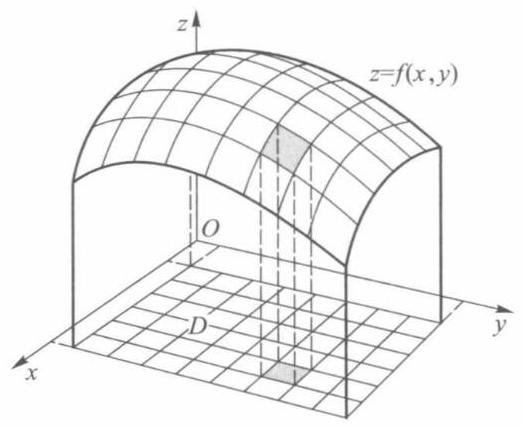
\includegraphics[width=.3\textwidth]{images/P156.jpg}
	\caption{图 $21-2$}
	\label{fig:P156}
\end{figure}

\begin{figure}
	\centering
	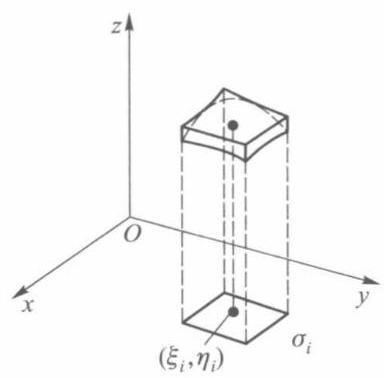
\includegraphics[width=.3\textwidth]{images/P157.jpg}
	\caption{图 $21-3$}
	\label{fig:P157}
\end{figure}


\[
\Delta {V}_{i} \approx  f\left( {{\xi }_{i},{\eta }_{i}}\right) \Delta {\sigma }_{i}.
\]
把这些小平顶柱体的体积加起来,就得到曲顶柱体体积 \(V\) 的近似值
\[
V = \mathop{\sum }\limits_{{i = 1}}^{n}\Delta {V}_{i} \approx  \mathop{\sum }\limits_{{i = 1}}^{n}f\left( {{\xi }_{i},{\eta }_{i}}\right) \Delta {\sigma }_{i}.
\]
当直线网 \(T\) 的网眼越来越细密,即分割 \(T\) 的细度 \(\parallel T\parallel  = \mathop{\max }\limits_{{1 \leq  i \leq  n}}{d}_{i}\left( {d}_{i}\right.\) 为 \({\sigma }_{i}\) 的直径) 趋于零时, 就有
\[
\mathop{\sum }\limits_{{i = 1}}^{n}f\left( {{\xi }_{i},{\eta }_{i}}\right) \Delta {\sigma }_{i} \rightarrow  V.
\]
至此,读者已经看到,求曲顶柱体的体积也与定积分概念一样,是通过“分割、近似求和、取极限”这三个步骤得到的, 所不同的是现在讨论的对象为定义在平面区域上的二元函数. 这类问题在物理学与工程技术中也常遇到, 如求非均匀平面的质量、质心、 转动惯量等. 这些都是所要讨论的二重积分的实际背景.

下面叙述定义在平面有界闭区域上函数 \(f\left( {x,y}\right)\) 的二重积分的概念.

设 \(D\) 为 \({xy}\) 平面上可求面积的有界闭区域, \(f\left( {x,y}\right)\) 为定义在 \(D\) 上的函数. 用任意的曲线把 \(D\) 分成 \(n\) 个可求面积的小区域
\[
{\sigma }_{1},{\sigma }_{2},\cdots ,{\sigma }_{n}.
\]
以 \(\Delta {\sigma }_{i}\) 表示小区域 \({\sigma }_{i}\) 的面积,这些小区域构成 \(D\) 的一个分割 \(T\) ,以 \({d}_{i}\) 表示小区域 \({\sigma }_{i}\) 的直径,称 \(\parallel T\parallel  = \mathop{\max }\limits_{{1 \leq  i \leq  n}}{d}_{i}\) 为分割 \(T\) 的细度. 在每个 \({\sigma }_{i}\) 上任取一点 \(\left( {{\xi }_{i},{\eta }_{i}}\right)\) ,作和式
\[
\mathop{\sum }\limits_{{i = 1}}^{n}f\left( {{\xi }_{i},{\eta }_{i}}\right) \Delta {\sigma }_{i}.
\]
称它为函数 \(f\left( {x,y}\right)\) 在 \(D\) 上属于分割 \(T\) 的一个积分和, \(\left( {{\xi }_{i},{\eta }_{i}}\right)\) 称为介点.

%定义  2
\begin{definition}{}{def:}

\end{definition}
设 \(f\left( {x,y}\right)\) 是定义在可求面积的有界闭区域 \(D\) 上的函数. \(J\) 是一个确定的数,若对任给的正数 \(\varepsilon\) ,总存在某个正数 \(\delta\) ,使对于 \(D\) 的任何分割 \(T\) ,当它的细度 \(\parallel T\parallel  <\)  \(\delta\) 时,属于 \(T\) 的所有积分和都有
\[
\left| {\mathop{\sum }\limits_{{i = 1}}^{n}f\left( {{\xi }_{i},{\eta }_{i}}\right) \Delta {\sigma }_{i} - J}\right|  < \varepsilon , \tag{4}
\]
则称 \(f\left( {x,y}\right)\) 在 \(D\) 上可积,数 \(J\) 称为函数 \(f\left( {x,y}\right)\) 在 \(D\) 上的二重积分,记作
\[
J = {\iint }_{D}f\left( {x,y}\right) \mathrm{d}\sigma , \tag{5}
\]
其中 \(f\left( {x,y}\right)\) 称为二重积分的被积函数, \(x,y\) 称为积分变量, \(D\) 称为积分区域.

当 \(f\left( {x,y}\right)  \geq  0\) 时,二重积分 \({\iint }_{D}f\left( {x,y}\right) \mathrm{d}\sigma\) 在几何上就表示以 \(z = f\left( {x,y}\right)\) 为曲顶, \(D\) 为底的曲顶柱体的体积. 当 \(f\left( {x,y}\right)  = 1\) 时,二重积分 \({\iint }_{D}f\left( {x,y}\right) \mathrm{d}\sigma\) 的值就等于积分区域 \(D\) 的面积.

由二重积分的定义知道,若 \(f\left( {x,y}\right)\) 在区域 \(D\) 上可积,则与定积分情况一样,对任何分割 \(T\) ,只要当 \(\parallel T\parallel  < \delta\) 时,(4) 式都成立. 因此为方便计算,常选取一些特殊的分割方法,如选用平行于坐标轴的直线网来分割 \(D\) ,则每一小网眼区域 \(\sigma\) 的面积 \({\Delta \sigma } = {\Delta x\Delta y}\) .

此时通常把 \({\iint }_{D}f\left( {x,y}\right) \mathrm{d}\sigma\) 记作
\[
{\iint }_{D}f\left( {x,y}\right) \mathrm{d}x\mathrm{\;d}y. \tag{6}
\]
首先可以像定积分那样类似地证明函数 \(f\left( {x,y}\right)\) 在有界、可求面积区域 \(D\) 上可积的必要条件是它在 \(D\) 上有界.

设函数 \(f\left( {x,y}\right)\) 在 \(D\) 上有界, \(T\) 为 \(D\) 的一个分割,它把 \(D\) 分成 \(n\) 个可求面积的小区域 \({\sigma }_{1},{\sigma }_{2},\cdots ,{\sigma }_{n}\) . 令
\[
\begin{array}{l} {M}_{i} = \mathop{\sup }\limits_{{\left( {x,y}\right)  \in  {\sigma }_{i}}}f\left( {x,y}\right) , \\  {m}_{i} = \mathop{\inf }\limits_{{\left( {x,y}\right)  \in  {\sigma }_{i}}}f\left( {x,y}\right)  \end{array}\;\left( {i = 1,2,\cdots ,n}\right) .
\]
作和式 \(S\left( T\right)  = \mathop{\sum }\limits_{{i = 1}}^{n}{M}_{i}\Delta {\sigma }_{i},s\left( T\right)  = \mathop{\sum }\limits_{{i = 1}}^{n}{m}_{i}\Delta {\sigma }_{i}\) . 它们分别称为函数 \(f\left( {x,y}\right)\) 关于分割 \(T\) 的上和与下和. 二元函数的上和与下和具有与一元函数的上和与下和同样的性质, 这里就不再重复. 下面列出有关二元函数的可积性定理. 我们只给出定理 21.7 的证明, 其余请读者自行证明.

定理 \({21.4f}\left( {x,y}\right)\) 在 \(D\) 上可积的充要条件是:
\[
\mathop{\lim }\limits_{{\parallel T\parallel  \rightarrow  0}}S\left( T\right)  = \mathop{\lim }\limits_{{\parallel T\parallel  \rightarrow  0}}s\left( T\right) .
\]
%定理 21.5
\begin{theorem}{}{the:}

\end{theorem}
 \(f\left( {x,y}\right)\) 在 \(D\) 上可积的充要条件是: 对于任给的正数 \(\varepsilon\) ,存在 \(D\) 的某个分割 \(T\) ,使得 \(S\left( T\right)  - s\left( T\right)  < \varepsilon\) .

%定理 21.6
\begin{theorem}{}{the:}

\end{theorem}
 有界闭区域 \(D\) 上的连续函数必可积.

%定理 21.7
\begin{theorem}{}{the:}

\end{theorem}
 设 \(f\left( {x,y}\right)\) 在有界闭域 \(D\) 上有界,且其不连续点集 \(E\) 是零面积集,则 \(f\left( {x,y}\right)\) 在 \(D\) 上可积.

%证
\begin{proof}

\end{proof}
对任意 \(\varepsilon  > 0\) ,存在有限个矩形 (不含边界) 覆盖了 \(E\) ,而这些矩形面积之和小于 \(\varepsilon\) . 记这些矩形之并集为 \(K\) ,则 \(D \smallsetminus  K\) 是有界闭域 (也可能是有限多个不交的有界闭域的并集). 设 \(K \cap  D\) 的面积为 \({\Delta }_{K}\) ,则 \({\Delta }_{K} < \varepsilon\) . 由于 \(f\left( {x,y}\right)\) 在 \(D \smallsetminus  K\) 上连续,因此由定理 21.6 和定理 21.5,存在 \(D \smallsetminus  K\) 上的分割 \({T}_{1} = \left\{  {{\sigma }_{1},{\sigma }_{2},\cdots ,{\sigma }_{n}}\right\}\) ,使得 \(S\left( {T}_{1}\right)  - s\left( {T}_{1}\right)  < \varepsilon\) . 令 \(T =\)  \(\left\{  {{\sigma }_{1},{\sigma }_{2},\cdots ,{\sigma }_{n},K \cap  D}\right\}\) ,则 \(T\) 是 \(D\) 的一个分割. 且
\[
S\left( T\right)  - s\left( T\right)  = S\left( {T}_{1}\right)  - s\left( {T}_{1}\right)  + {\omega }_{K}{\Delta }_{K} < \varepsilon  + {\omega \varepsilon },
\]
其中 \({\omega }_{K}\) 是 \(f\left( {x,y}\right)\) 在 \(K \cap  D\) 上的振幅, \(\omega\) 是 \(f\left( {x,y}\right)\) 在 \(D\) 上的振幅. 由定理 21.5, \(f\left( {x,y}\right)\) 在 \(D\) 上可积.

\subsection{二重积分的性质}

二重积分具有一系列与定积分完全相类似的性质, 现列举如下.

1. 若 \(f\left( {x,y}\right)\) 在区域 \(D\) 上可积, \(k\) 为常数,则 \({kf}\left( {x,y}\right)\) 在 \(D\) 上也可积,且
\[
{\iint }_{D}{kf}\left( {x,y}\right) \mathrm{d}\sigma  = k{\iint }_{D}f\left( {x,y}\right) \mathrm{d}\sigma .
\]
2. 若 \(f\left( {x,y}\right) ,g\left( {x,y}\right)\) 在 \(D\) 上都可积,则 \(f\left( {x,y}\right)  \pm  g\left( {x,y}\right)\) 在 \(D\) 上也可积,且
\[
{\iint }_{D}\left\lbrack  {f\left( {x,y}\right)  \pm  g\left( {x,y}\right) }\right\rbrack  \mathrm{d}\sigma  = {\iint }_{D}f\left( {x,y}\right) \mathrm{d}\sigma  \pm  {\iint }_{D}g\left( {x,y}\right) \mathrm{d}\sigma .
\]
3. 若 \(f\left( {x,y}\right)\) 在 \({D}_{1}\) 和 \({D}_{2}\) 上都可积,且 \({D}_{1}\) 与 \({D}_{2}\) 无公共内点,则 \(f\left( {x,y}\right)\) 在 \({D}_{1} \cup  {D}_{2}\) 上也可积,且
\[
{\iint }_{{D}_{1} \cup  {D}_{2}}f\left( {x,y}\right) \mathrm{d}\sigma  = {\iint }_{{D}_{1}}f\left( {x,y}\right) \mathrm{d}\sigma  + {\iint }_{{D}_{2}}f\left( {x,y}\right) \mathrm{d}\sigma .
\]
4. 若 \(f\left( {x,y}\right)\) 与 \(g\left( {x,y}\right)\) 在 \(D\) 上可积,且
\[
f\left( {x,y}\right)  \leq  g\left( {x,y}\right) ,\;\left( {x,y}\right)  \in  D,
\]
则
\[
{\iint }_{D}f\left( {x,y}\right) \mathrm{d}\sigma  \leq  {\iint }_{D}g\left( {x,y}\right) \mathrm{d}\sigma .
\]
5. 若 \(f\left( {x,y}\right)\) 在 \(D\) 上可积,则函数 \(\left| {f\left( {x,y}\right) }\right|\) 在 \(D\) 上也可积,且
\[
\left| {{\iint }_{D}f\left( {x,y}\right) \mathrm{d}\sigma }\right|  \leq  {\iint }_{D}\left| {f\left( {x,y}\right) }\right| \mathrm{d}\sigma .
\]
6. 若 \(f\left( {x,y}\right)\) 在 \(D\) 上可积,且
\[
m \leq  f\left( {x,y}\right)  \leq  M,\;\left( {x,y}\right)  \in  D,
\]
则
\[
m{S}_{D} \leq  {\iint }_{D}f\left( {x,y}\right) \mathrm{d}\sigma  \leq  M{S}_{D},
\]
这里 \({S}_{D}\) 是积分区域 \(D\) 的面积.

7. (中值定理) 若 \(f\left( {x,y}\right)\) 在有界闭区域 \(D\) 上连续,则存在 \(\left( {\xi ,\eta }\right)  \in  D\) ,使得
\[
{\iint }_{D}f\left( {x,y}\right) \mathrm{d}\sigma  = f\left( {\xi ,\eta }\right) {S}_{D},
\]
这里 \({S}_{D}\) 是积分区域 \(D\) 的面积.

中值定理的几何意义: 以 \(D\) 为底, \(z = f\left( {x,y}\right) \left( {f\left( {x,y}\right)  \geq  0}\right)\) 为曲顶的曲顶柱体体积等于一个同底的平顶柱体的体积,这个平顶柱体的高等于 \(f\left( {x,y}\right)\) 在区域 \(D\) 中某点 \(\left( {\xi ,\eta }\right)\) 的函数值 \(f\left( {\xi ,\eta }\right)\) .

\subsection{习题 21.1}

1. 把重积分 \({\iint }_{D}{xy}\mathrm{\;d}\sigma\) 作为积分和的极限,计算这个积分值,其中 \(D = \left\lbrack  {0,1}\right\rbrack   \times  \left\lbrack  {0,1}\right\rbrack\) ,并用直线网
\[
x = \frac{i}{n},y = \frac{j}{n}\;\left( {i,j = 1,2,\cdots ,n - 1}\right)
\]
分割这个正方形为许多小正方形, 每个小正方形取其右上顶点作为其介点.

2. 证明: 若函数 \(f\left( {x,y}\right)\) 在有界闭区域 \(D\) 上可积,则 \(f\left( {x,y}\right)\) 在 \(D\) 上有界.

3. 证明二重积分中值定理 (性质 7).

4. 若 \(f\left( {x,y}\right)\) 为有界闭区域 \(D\) 上的非负连续函数,且在 \(D\) 上不恒为零,则
\[
{\iint }_{D}f\left( {x,y}\right) \mathrm{d}\sigma  > 0.
\]
5. 若 \(f\left( {x,y}\right)\) 在有界闭区域 \(D\) 上连续,且在 \(D\) 内任一子区域 \({D}^{\prime } \subset  D\) 上有
\[
{\iint }_{{D}^{\prime }}f\left( {x,y}\right) \mathrm{d}\sigma  = 0,
\]
则在 \(D\) 上 \(f\left( {x,y}\right)  \equiv  0\) .

6. 设 \(D = \left\lbrack  {0,1}\right\rbrack   \times  \left\lbrack  {0,1}\right\rbrack\) ,证明函数
\[
f\left( {x,y}\right)  = \left\{  \begin{array}{ll} 1, & \left( {x,y}\right) \text{ 为 }D\text{ 内有理点 ( 即 }x,y\text{ 皆为有理数 }), \\  0, & \left( {x,y}\right) \text{ 为 }D\text{ 内非有理点 } \end{array}\right.
\]
在 \(D\) 上不可积.

7. 证明: 若 \(f\left( {x,y}\right)\) 在有界闭区域 \(D\) 上连续, \(g\left( {x,y}\right)\) 在 \(D\) 上可积且不变号,则存在一点 \(\left( {\xi ,\eta }\right)  \in\)  \(D\) ,使得
\[
{\iint }_{D}f\left( {x,y}\right) g\left( {x,y}\right) \mathrm{d}\sigma  = f\left( {\xi ,\eta }\right) {\iint }_{D}g\left( {x,y}\right) \mathrm{d}\sigma .
\]
8. 应用中值定理估计积分
\[
I = {\iint }_{\left| x\right|  + \left| y\right|  \leq  {10}}\frac{\mathrm{d}\sigma }{{100} + {\cos }^{2}x + {\cos }^{2}y}
\]
的值.

\section{直角坐标系下二重积分的计算}

本节首先讨论定义在矩形区域 \(D = \left\lbrack  {a,b}\right\rbrack   \times  \left\lbrack  {c,d}\right\rbrack\) 上二重积分计算问题,然后再把它扩展到较为一般的区域上.

%定理 21.8
\begin{theorem}{}{the:}

\end{theorem}
 设 \(f\left( {x,y}\right)\) 在矩形区域 \(D = \left\lbrack  {a,b}\right\rbrack   \times  \left\lbrack  {c,d}\right\rbrack\) 上可积,且对每个 \(x \in  \left\lbrack  {a,b}\right\rbrack\) , 积分 \({\int }_{c}^{d}f\left( {x,y}\right) \mathrm{d}y\) 存在,则累次积分
\[
{\int }_{a}^{b}\mathrm{\;d}x{\int }_{c}^{d}f\left( {x,y}\right) \mathrm{d}y
\]
也存在, 且
\[
{\iint }_{D}f\left( {x,y}\right) \mathrm{d}\sigma  = {\int }_{a}^{b}\mathrm{\;d}x{\int }_{c}^{d}f\left( {x,y}\right) \mathrm{d}y. \tag{1}
\]
%证
\begin{proof}

\end{proof}
令 \(F\left( x\right)  = {\int }_{c}^{d}f\left( {x,y}\right) \mathrm{d}y\) ,定理要求证明 \(F\left( x\right)\) 在 \(\left\lbrack  {a,b}\right\rbrack\) 上可积,且积分的结果恰为二重积分. 为此,对区间 \(\left\lbrack  {a,b}\right\rbrack\) 与 \(\left\lbrack  {c,d}\right\rbrack\) 分别作分割
\[
a = {x}_{0} < {x}_{1} < \cdots  < {x}_{r} = b,
\]
\[
c = {y}_{0} < {y}_{1} < \cdots  < {y}_{s} = d.
\]
\begin{figure}
	\centering
	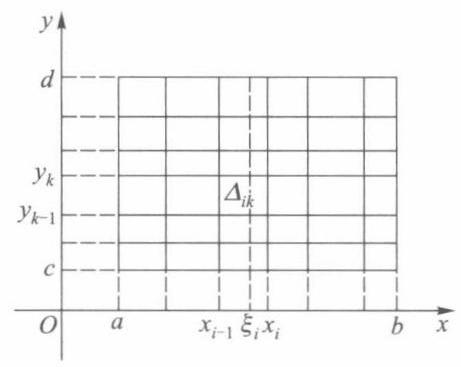
\includegraphics[width=.3\textwidth]{images/P158.jpg}
	\caption{图 $21-4$}
	\label{fig:P158}
\end{figure}

按这些分点作两组直线
\[
x = {x}_{i}\;\left( {i = 1,2,\cdots ,r - 1}\right)
\]
及
\[
y = {y}_{k}\;\left( {k = 1,2,\cdots ,s - 1}\right) ,
\]
它把矩形 \(D\) 分为 \({rs}\) 个小矩形 (图 21-4). 记 \({\Delta }_{ik}\) 为小矩形 \(\left\lbrack  {{x}_{i - 1},{x}_{i}}\right\rbrack   \times  \left\lbrack  {{y}_{k - 1},{y}_{k}}\right\rbrack  \;\left( {i = 1,2,\cdots ,r,k = 1,2,\cdots ,s}\right)\) ; 设 \(f\left( {x,y}\right)\) 在 \({\Delta }_{ik}\) 上的上确界和下确界分别为 \({M}_{ik}\) 和 \({m}_{ik}\) . 在区间 \(\left\lbrack  {{x}_{i - 1},{x}_{i}}\right\rbrack\) 中任取一点 \({\xi }_{i}\) , 于是就有不等式
\[
{m}_{ik}\Delta {y}_{k} \leq  {\int }_{{y}_{k - 1}}^{{y}_{k}}f\left( {{\xi }_{i},y}\right) \mathrm{d}y \leq  {M}_{ik}\Delta {y}_{k},
\]
其中 \(\Delta {y}_{k} = {y}_{k} - {y}_{k - 1}\) . 因此
\[
\mathop{\sum }\limits_{{k = 1}}^{s}{m}_{ik}\Delta {y}_{k} \leq  F\left( {\xi }_{i}\right)  = {\int }_{c}^{d}f\left( {{\xi }_{i},y}\right) \mathrm{d}y \leq  \mathop{\sum }\limits_{{k = 1}}^{s}{M}_{ik}\Delta {y}_{k},
\]
\[
\mathop{\sum }\limits_{{i = 1}}^{r}\mathop{\sum }\limits_{{k = 1}}^{s}{m}_{ik}\Delta {y}_{k}\Delta {x}_{i} \leq  \mathop{\sum }\limits_{{i = 1}}^{r}F\left( {\xi }_{i}\right) \Delta {x}_{i} \leq  \mathop{\sum }\limits_{{i = 1}}^{r}\mathop{\sum }\limits_{{k = 1}}^{s}{M}_{ik}\Delta {y}_{k}\Delta {x}_{i}, \tag{2}
\]
其中 \(\Delta {x}_{i} = {x}_{i} - {x}_{i - 1}\) . 记 \({\Delta }_{ik}\) 的对角线长度为 \({d}_{ik}\) 和
\[
\parallel T\parallel  = \mathop{\max }\limits_{{i,k}}{d}_{ik}.
\]
由于二重积分存在,由定理 21.4,当 \(\parallel T\parallel  \rightarrow  0\) 时, \(\mathop{\sum }\limits_{{i,k}}{m}_{ik}\Delta {y}_{k}\Delta {x}_{i}\) 和 \(\mathop{\sum }\limits_{{i,k}}{M}_{ik}\Delta {y}_{k}\Delta {x}_{i}\) 有相同的极限,且极限值等于 \({\iint }_{D}f\left( {x,y}\right) \mathrm{d}\sigma\) . 因此当 \(\parallel T\parallel  \rightarrow  0\) 时,由不等式 (2) 可得
\[
\mathop{\lim }\limits_{{\parallel T\parallel  \rightarrow  0}}\mathop{\sum }\limits_{{i = 1}}^{r}F\left( {\xi }_{i}\right) \Delta {x}_{i} = {\iint }_{D}f\left( {x,y}\right) \mathrm{d}\sigma . \tag{3}
\]
由于当 \(\parallel T\parallel  \rightarrow  0\) 时,必有 \(\mathop{\max }\limits_{{1 \leq  i \leq  r}}\Delta {x}_{i} \rightarrow  0\) ,因此由定积分定义,(3) 式左边
\[
\mathop{\lim }\limits_{{\parallel T\parallel  \rightarrow  0}}\mathop{\sum }\limits_{{i = 1}}^{r}F\left( {\xi }_{i}\right) \Delta {x}_{i} = {\int }_{a}^{b}F\left( x\right) \mathrm{d}x = {\int }_{a}^{b}\mathrm{\;d}x{\int }_{c}^{d}f\left( {x,y}\right) \mathrm{d}y.
\]
%定理 21.9
\begin{theorem}{}{the:}

\end{theorem}
 设 \(f\left( {x,y}\right)\) 在矩形区域 \(D = \left\lbrack  {a,b}\right\rbrack   \times  \left\lbrack  {c,d}\right\rbrack\) 上可积,且对每个 \(y \in  \left\lbrack  {c,d}\right\rbrack\) , 积分 \({\int }_{a}^{b}f\left( {x,y}\right) \mathrm{d}x\) 存在,则累次积分
\[
{\int }_{c}^{d}\mathrm{\;d}y{\int }_{a}^{b}f\left( {x,y}\right) \mathrm{d}x
\]
也存在, 且
\[
{\iint }_{D}f\left( {x,y}\right) \mathrm{d}\sigma  = {\int }_{c}^{d}\mathrm{\;d}y{\int }_{a}^{b}f\left( {x,y}\right) \mathrm{d}x.
\]
%定理 21.9
\begin{theorem}{}{the:}

\end{theorem}
 的证明与定理 21.8 相仿.

特别当 \(f\left( {x,y}\right)\) 在矩形区域 \(D = \left\lbrack  {a,b}\right\rbrack   \times  \left\lbrack  {c,d}\right\rbrack\) 上连续时,则有
\[
{\iint }_{D}f\left( {x,y}\right) \mathrm{d}\sigma  = {\int }_{a}^{b}\mathrm{\;d}x{\int }_{c}^{d}f\left( {x,y}\right) \mathrm{d}y = {\int }_{c}^{d}\mathrm{\;d}y{\int }_{a}^{b}f\left( {x,y}\right) \mathrm{d}x.
\]
%例 1
\begin{example}

\end{example}
计算 \({\iint }_{D}y\sin \left( {xy}\right) \mathrm{d}x\mathrm{\;d}y\) ,其中 \(D = \left\lbrack  {0,\pi }\right\rbrack   \times  \left\lbrack  {0,1}\right\rbrack\) .

%解
\begin{solution}

\end{solution}
\({\iint }_{D}y\sin \left( {xy}\right) \mathrm{d}x\mathrm{\;d}y = {\int }_{0}^{1}\mathrm{\;d}y{\int }_{0}^{\pi }y\sin \left( {xy}\right) \mathrm{d}x = {\int }_{0}^{1}\mathrm{\;d}y{\int }_{0}^{\pi }\frac{\partial }{\partial x}\left( {-\cos \left( {xy}\right) }\right) \mathrm{d}x\)
\[
=  - {\left. {\int }_{0}^{1}\cos \left( xy\right) \right| }_{0}^{\pi }\mathrm{d}y = {\int }_{0}^{1}\left( {1 - \cos \left( {\pi y}\right) }\right) \mathrm{d}y
\]
\[
= 1 - {\left. \frac{1}{\pi }\sin \left( \pi y\right) \right| }_{0}^{1} = 1.
\]
对于一般区域, 通常可以分解为如下两类区域来进行计算.

称平面点集
\[
D = \left\{  {\left( {x,y}\right)  \mid  {y}_{1}\left( x\right)  \leq  y \leq  {y}_{2}\left( x\right) ,a \leq  x \leq  b}\right\}   \tag{4}
\]
为 \(x\) 型区域 (图 21-5(a)) ; 称平面点集
\[
D = \left\{  {\left( {x,y}\right)  \mid  {x}_{1}\left( y\right)  \leq  x \leq  {x}_{2}\left( y\right) ,c \leq  y \leq  d}\right\}   \tag{5}
\]
为 \(y\) 型区域 (图 21-5(b)).

\begin{figure}
	\centering
	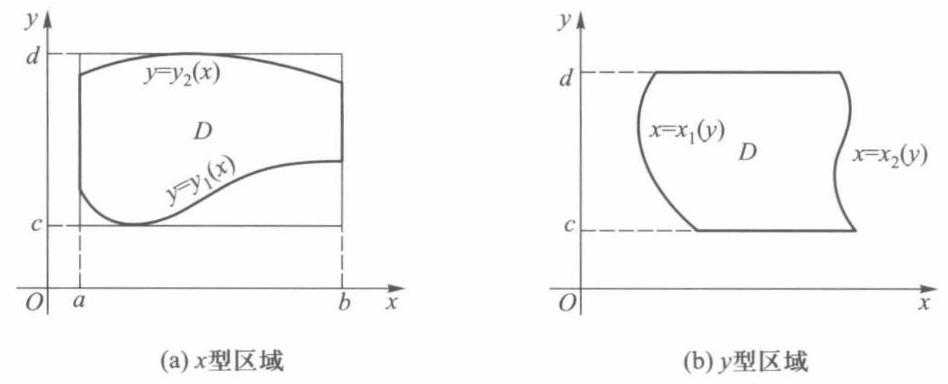
\includegraphics[width=.3\textwidth]{images/P159.jpg}
	\caption{图 $21-5$}
	\label{fig:P159}
\end{figure}

这些区域的特点是当 \(D\) 为 \(x\) 型区域时,垂直于 \(x\) 轴的直线 \(x = {x}_{0}\left( {a < {x}_{0} < b}\right)\) 至多与区域 \(D\) 的边界交于两点; 当 \(D\) 为 \(y\) 型区域时,直线 \(y = {y}_{0}\left( {c < {y}_{0} < d}\right)\) 至多与 \(D\) 的边界交于两点.

许多常见的区域都可以分解成有限个除边界外无公共内点的 \(x\) 型区域或 \(y\) 型区域 (如图 21-6 所示的区域 \(D\) 可分解成三个区域,其 I, III为 \(x\) 型区域, II 为 \(y\) 型区域). 因而解决了 \(x\) 型区域或 \(y\) 型区域上二重积分的计算问题, 那么一般区域上二重积分的计算问题也就得到了解决.

\begin{figure}
	\centering
	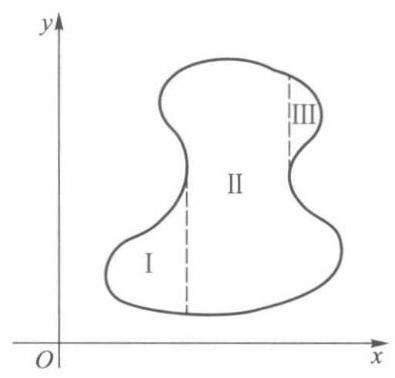
\includegraphics[width=.3\textwidth]{images/P160.jpg}
	\caption{图 $21-6$}
	\label{fig:P160}
\end{figure}

%定理 21.10
\begin{theorem}{}{the:}

\end{theorem}
 若 \(f\left( {x,y}\right)\) 在如 (4) 式所示的 \(x\) 型区域 \(D\) 上连续,其中 \({y}_{1}\left( x\right) ,{y}_{2}\left( x\right)\) 在 \(\left\lbrack  {a,b}\right\rbrack\) 上连续,则
\[
{\iint }_{D}f\left( {x,y}\right) \mathrm{d}\sigma  = {\int }_{a}^{b}\mathrm{\;d}x{\int }_{{y}_{1}\left( x\right) }^{{y}_{2}\left( x\right) }f\left( {x,y}\right) \mathrm{d}y.
\]
即二重积分可化为先对 \(y\) 后对 \(x\) 的累次积分.

%证
\begin{proof}

\end{proof}
由于 \({y}_{1}\left( x\right)\) 与 \({y}_{2}\left( x\right)\) 在闭区间 \(\left\lbrack  {a,b}\right\rbrack\) 上连续,故存在矩形区域 \(\left\lbrack  {a,b}\right\rbrack   \times  \left\lbrack  {c,d}\right\rbrack   \supset\)  \(D\) (如图 \({21} - 5\left( \mathrm{a}\right)\) ),现作一定义在 \(\left\lbrack  {a,b}\right\rbrack   \times  \left\lbrack  {c,d}\right\rbrack\) 上的函数
\[
F\left( {x,y}\right)  = \left\{  \begin{array}{ll} f\left( {x,y}\right) , & \left( {x,y}\right)  \in  D, \\  0, & \left( {x,y}\right)  \notin  D. \end{array}\right.
\]
可以验证,函数 \(F\left( {x,y}\right)\) 在 \(\left\lbrack  {a,b}\right\rbrack   \times  \left\lbrack  {c,d}\right\rbrack\) 上可积,而且
\[
{\iint }_{D}f\left( {x,y}\right) \mathrm{d}\sigma  = {\iint }_{\left\lbrack  {a,b}\right\rbrack   \times  \left\lbrack  {c,d}\right\rbrack  }F\left( {x,y}\right) \mathrm{d}\sigma  = {\int }_{a}^{b}\mathrm{\;d}x{\int }_{c}^{d}F\left( {x,y}\right) \mathrm{d}y
\]
\[
= {\int }_{a}^{b}\mathrm{\;d}x{\int }_{{y}_{1}\left( x\right) }^{{y}_{2}\left( x\right) }F\left( {x,y}\right) \mathrm{d}y = {\int }_{a}^{b}\mathrm{\;d}x{\int }_{{y}_{1}\left( x\right) }^{{y}_{2}\left( x\right) }f\left( {x,y}\right) \mathrm{d}y.
\]
%注
\begin{remark}

\end{remark}
从几何意义上可以这样来理解化二重积分为累次积分,二重积分是计算以 \(D\) 为底面, \(f\left( {x,y}\right) \left( { \geq  0}\right)\) 为高的曲顶柱体的体积,这个曲顶柱体可视为介于平行平面 \(x = a\) 与 \(x = b\) 之间的立体, 可以利用截面面积 \(S\left( x\right) ,x \in  \left\lbrack  {a,b}\right\rbrack\) 的积分求出. 而截面面积 \(S\left( x\right)\) 是一元函数 \(f\left( {x,y}\right)\) (其中 \(x\) 为参量)与 \(y\) 轴以及直线 \(y = {y}_{1}\left( x\right) ,y = {y}_{2}\left( x\right)\) 所围图形的面积 (图 21-7), 所以
\[
S\left( x\right)  = {\int }_{{y}_{1}\left( x\right) }^{{y}_{2}\left( x\right) }f\left( {x,y}\right) \mathrm{d}y.
\]
\begin{figure}
	\centering
	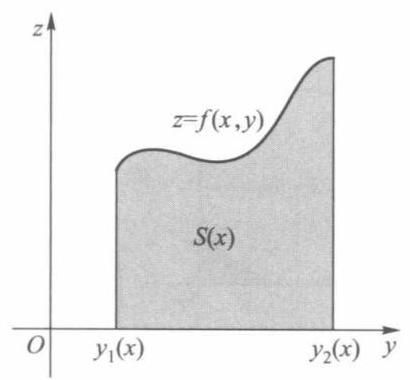
\includegraphics[width=.3\textwidth]{images/P161.jpg}
	\caption{图 $21-7$}
	\label{fig:P161}
\end{figure}

那么曲顶柱体的体积
\[
V = {\int }_{a}^{b}S\left( x\right) \mathrm{d}x = {\int }_{a}^{b}\mathrm{\;d}x{\int }_{{y}_{1}\left( x\right) }^{{y}_{2}\left( x\right) }f\left( {x,y}\right) \mathrm{d}y.
\]
类似可证,若 \(D\) 为 (5) 式所示的 \(y\) 型区域,其中 \({x}_{1}\left( y\right) ,{x}_{2}\left( y\right)\) 在 \(\left\lbrack  {c,d}\right\rbrack\) 上连续,则二重积分可化为先对 \(x\) 后对 \(y\) 的累次积分
\[
{\iint }_{D}f\left( {x,y}\right) \mathrm{d}\sigma  = {\int }_{c}^{d}\mathrm{\;d}y{\int }_{{x}_{1}\left( y\right) }^{{x}_{2}\left( y\right) }f\left( {x,y}\right) \mathrm{d}x.
\]
%例 2
\begin{example}

\end{example}
设 \(D\) 是由直线 \(x = 0,y = 1\) 及 \(y = x\) 围成的区域 (图 21-8),试计算 \(I = {\iint }_{D}{x}^{2}{\mathrm{e}}^{-{y}^{2}}\mathrm{\;d}\sigma\) 的值.

%解
\begin{solution}

\end{solution}
若用先对 \(y\) 后对 \(x\) 的积分,则
\[
I = {\int }_{0}^{1}{x}^{2}\mathrm{\;d}x{\int }_{x}^{1}{\mathrm{e}}^{-{y}^{2}}\mathrm{\;d}y.
\]
由于函数 \({\mathrm{e}}^{-{y}^{2}}\) 的原函数无法用初等函数形式表示,因此改用另一种顺序的累次积分, 则有
\[
I = {\int }_{0}^{1}\mathrm{\;d}y{\int }_{0}^{y}{x}^{2}{\mathrm{e}}^{-{y}^{2}}\mathrm{\;d}x = \frac{1}{3}{\int }_{0}^{1}{y}^{3}{\mathrm{e}}^{-{y}^{2}}\mathrm{\;d}y.
\]
由分部积分法, 即可算得
\[
I = \frac{1}{6} - \frac{1}{3\mathrm{e}}
\]
%例 3
\begin{example}

\end{example}
计算二重积分 \({\iint }_{D}\mathrm{\;d}\sigma\) ,其中 \(D\) 为由直线 \(y = {2x},x = {2y}\) 及 \(x + y = 3\) 所围的三角形区域 (图 21-9).

\begin{figure}
	\centering
	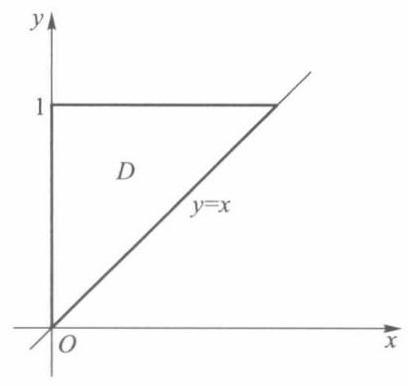
\includegraphics[width=.3\textwidth]{images/P162.jpg}
	\caption{图 $21-8$}
	\label{fig:P162}
\end{figure}

\begin{figure}
	\centering
	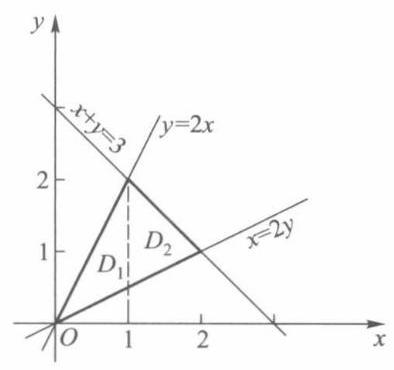
\includegraphics[width=.3\textwidth]{images/P163.jpg}
	\caption{图 $21-9$}
	\label{fig:P163}
\end{figure}

%解
\begin{solution}

\end{solution}
当把 \(D\) 看作 \(x\) 型区域时,相应的
\[
{y}_{2}\left( x\right)  = \left\{  {\begin{array}{ll} {2x}, & 0 \leq  x \leq  1, \\  3 - x, & 1 < x \leq  2, \end{array}\;{y}_{1}\left( x\right)  = \frac{x}{2}.}\right.
\]
所以
\[
{\iint }_{D}\mathrm{\;d}\sigma  = {\iint }_{{D}_{1}}\mathrm{\;d}\sigma  + {\iint }_{{D}_{2}}\mathrm{\;d}\sigma  = {\int }_{0}^{1}\mathrm{\;d}x{\int }_{\frac{x}{2}}^{2x}\mathrm{\;d}y + {\int }_{1}^{2}\mathrm{\;d}x{\int }_{\frac{x}{2}}^{3 - x}\mathrm{\;d}y
\]
\[
= {\int }_{0}^{1}\left( {{2x} - \frac{x}{2}}\right) \mathrm{d}x + {\int }_{1}^{2}\left( {3 - x - \frac{x}{2}}\right) \mathrm{d}x
\]
\[
= {\left. \left\lbrack  \frac{3}{4}{x}^{2}\right\rbrack  \right| }_{0}^{1} + {\left. \left\lbrack  3x - \frac{3}{4}{x}^{2}\right\rbrack  \right| }_{1}^{2} = \frac{3}{2}.
\]
%例 4
\begin{example}

\end{example}
求两个底面半径相同的直交圆柱所围立体的体积 \(V\) .

%解
\begin{solution}

\end{solution}
设圆柱底面半径为 \(a\) ,两个圆柱方程为
\[
{x}^{2} + {y}^{2} = {a}^{2}\text{ 与 }{x}^{2} + {z}^{2} = {a}^{2}.
\]
利用对称性,只要求出在第一卦限 (即 \(x \geq  0,y \geq  0,z \geq  0\) ) 部分 (见第十章图 10-10) 的体积,然后再乘以 8 即得所求的体积. 第一卦限部分的立体是以 \(z = \sqrt{{a}^{2} - {x}^{2}}\) 为曲顶,以四分之一圆域
\[
D : \left\{  \begin{array}{l} 0 \leq  y \leq  \sqrt{{a}^{2} - {x}^{2}}, \\  0 \leq  x \leq  a \end{array}\right.
\]
为底的曲顶柱体, 所以
\[
\frac{1}{8}V = {\iint }_{D}\sqrt{{a}^{2} - {x}^{2}}\mathrm{\;d}\sigma  = {\int }_{0}^{a}\mathrm{\;d}x{\int }_{0}^{\sqrt{{a}^{2} - {x}^{2}}}\sqrt{{a}^{2} - {x}^{2}}\mathrm{\;d}y
\]
\[
= {\int }_{0}^{a}\left( {{a}^{2} - {x}^{2}}\right) \mathrm{d}x = \frac{2}{3}{a}^{3}.
\]
于是 \(V = \frac{16}{3}{a}^{3}\) .

\subsection{习题 21.2}

1. 设 \(f\left( {x,y}\right)\) 在区域 \(D\) 上连续,试将二重积分 \({\iint }_{D}f\left( {x,y}\right) \mathrm{d}\sigma\) 化为不同顺序的累次积分:

(1) \(D\) 是由不等式 \(y \leq  x,y \geq  a,x \leq  b\left( {0 < a < b}\right)\) 所确定的区域；

(2) \(D\) 是由不等式 \(y \leq  x,y \geq  0,{x}^{2} + {y}^{2} \leq  1\) 所确定的区域；

(3) \(D\) 是由不等式 \({x}^{2} + {y}^{2} \leq  1\) 与 \(x + y \geq  1\) 所确定的区域；

(4) \(D = \{ \left( {x,y}\right) \left| \right| x\left| +\right| y \mid   \leq  1\}\) .

2. 在下列积分中改变累次积分的顺序:

(1) \({\int }_{0}^{2}\mathrm{\;d}x{\int }_{x}^{2x}f\left( {x,y}\right) \mathrm{d}y\) ;

(2) \({\int }_{-1}^{1}\mathrm{\;d}x{\int }_{-\sqrt{1 - {x}^{2}}}^{1 - {x}^{2}}f\left( {x,y}\right) \mathrm{d}y\) ;

(3) \({\int }_{0}^{2a}\mathrm{\;d}x{\int }_{\sqrt{{2ax} - {x}^{2}}}^{\sqrt{2ax}}f\left( {x,y}\right) \mathrm{d}y\) ;

(4) \({\int }_{0}^{1}\mathrm{\;d}x{\int }_{0}^{{x}^{2}}f\left( {x,y}\right) \mathrm{d}y + {\int }_{1}^{3}\mathrm{\;d}x{\int }_{0}^{\frac{1}{2}\left( {3 - x}\right) }f\left( {x,y}\right) \mathrm{d}y\) .

3. 计算下列二重积分:

(1) \({\iint }_{D}x{y}^{2}\mathrm{\;d}\sigma\) ,其中 \(D\) 是由抛物线 \({y}^{2} = {2px}\) 与直线 \(x = \frac{p}{2}\left( {p > 0}\right)\) 所围成的区域;

\begin{figure}
	\centering
	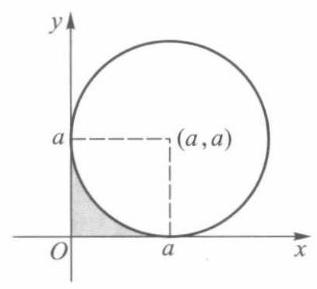
\includegraphics[width=.3\textwidth]{images/P164.jpg}
	\caption{图 $21-10$}
	\label{fig:P164}
\end{figure}

( 2 ) \({\iint }_{D}\left( {{x}^{2} + {y}^{2}}\right) \mathrm{d}\sigma\) ,其中 \(D = \left\{  {\left( {x,y}\right)  \mid  0 \leq  x \leq  1,\sqrt{x} \leq  y \leq  2\sqrt{x}}\right\}\) ；

(3) \({\iint }_{D}\frac{\mathrm{d}\sigma }{\sqrt{{2a} - x}}\left( {a > 0}\right)\) ,其中 \(D\) 为图 21-10 中阴影部分；

(4) \({\iint }_{D}\sqrt{x}\mathrm{\;d}\sigma\) ,其中 \(D = \left\{  {\left( {x,y}\right)  \mid  {x}^{2} + {y}^{2} \leq  x}\right\}\) .

4. 求由坐标平面及 \(x = 2,y = 3,x + y + z = 4\) 所围的角柱体的体积.

5. 设 \(f\left( x\right)\) 在 \(\left\lbrack  {a,b}\right\rbrack\) 上连续,证明不等式
\[
{\left\lbrack  {\int }_{a}^{b}f\left( x\right) \mathrm{d}x\right\rbrack  }^{2} \leq  \left( {b - a}\right) {\int }_{a}^{b}{f}^{2}\left( x\right) \mathrm{d}x,
\]
其中等号仅在 \(f\left( x\right)\) 为常量函数时成立.

6. 设平面区域 \(D\) 在 \(x\) 轴和 \(y\) 轴的投影长度分别为 \({l}_{x}\) 和 \({l}_{y},D\) 的面积为 \({S}_{D},\left( {\alpha ,\beta }\right)\) 为 \(D\) 内任一点, 证明:

(1) \(\left| {{\iint }_{D}\left( {x - \alpha }\right) \left( {y - \beta }\right) \mathrm{d}\sigma }\right|  \leq  {l}_{x}{l}_{y}{S}_{D}\) ;

(2) \(\left| {{\iint }_{D}\left( {x - \alpha }\right) \left( {y - \beta }\right) \mathrm{d}\sigma }\right|  \leq  \frac{1}{4}{l}_{x}^{2}{l}_{y}^{2}\) .

7. 设 \(D = \left\lbrack  {0,1}\right\rbrack   \times  \left\lbrack  {0,1}\right\rbrack\) ,
\[
f\left( {x,y}\right)  = \begin{cases} \frac{1}{{q}_{x}} + \frac{1}{{q}_{y}}, & \text{ 当 }\left( {x,y}\right) \text{ 为 }D\text{ 中有理点, } \\  0, & \text{ 当 }\left( {x,y}\right) \text{ 为 }D\text{ 中非有理点, } \end{cases}
\]
其中 \({q}_{x}\) 表示有理数 \(x\) 化成既约分数后的分母. 证明 \(f\left( {x,y}\right)\) 在 \(D\) 上的二重积分存在而两个累次积分不存在.

8. 设 \(D = \left\lbrack  {0,1}\right\rbrack   \times  \left\lbrack  {0,1}\right\rbrack\) ,
\[
f\left( {x,y}\right)  = \left\{  \begin{array}{ll} 1, & \text{ 当 }\left( {x,y}\right) \text{ 为 }D\text{ 中有理点,且 }{q}_{x} = {q}_{y}\text{ 时, } \\  0, & \text{ 当 }\left( {x,y}\right) \text{ 为 }D\text{ 中其他点时, } \end{array}\right.
\]
其中 \({q}_{x}\) 意义同第 7 题. 证明 \(f\left( {x,y}\right)\) 在 \(D\) 上的二重积分不存在而两个累次积分存在.

\section{格林公式 - 曲线积分与路线的无关性}

\subsection{格林公式}

本节讨论区域 \(D\) 上的二重积分与 \(D\) 的边界曲线 \(L\) 上的第二型曲线积分之间的联系.

设区域 \(D\) 的边界 \(L\) 由一条或几条光滑曲线所组成. 边界曲线的正方向规定为: 当人沿边界行走时,区域 \(D\) 总在他的左边,如图 21-11 所示. 与上述规定的方向相反的方向称为负方向,记为 \(- L\) .

\begin{figure}
	\centering
	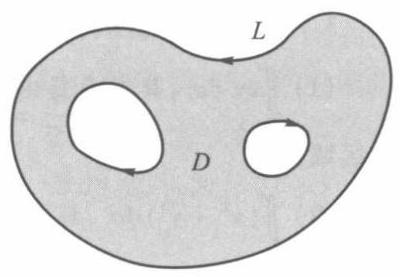
\includegraphics[width=.3\textwidth]{images/P165.jpg}
	\caption{图 $21-11$}
	\label{fig:P165}
\end{figure}

%定理 21.11
\begin{theorem}{}{the:}

\end{theorem}
 若函数 \(P\left( {x,y}\right) ,Q\left( {x,y}\right)\) 在闭区域 \(D\) 上连续, 且有连续的一阶偏导数, 则有
\[
{\iint }_{D}\left( {\frac{\partial Q}{\partial x} - \frac{\partial P}{\partial y}}\right) \mathrm{d}\sigma  = {\oint }_{L}P\mathrm{\;d}x + Q\mathrm{\;d}y, \tag{1}
\]
这里 \(L\) 为区域 \(D\) 的边界曲线,分段光滑,并取正方向.

公式 (1) 称为格林 (Green) 公式.

%证
\begin{proof}

\end{proof}
根据区域 \(D\) 的不同形状,一般可分三种情形来证明:

(i) 若区域 \(D\) 既是 \(x\) 型区域又是 \(y\) 型区域,即平行于坐标轴的直线和 \(L\) 至多交于两点 (图 21-12). 这时区域 \(D\) 可表示为
\[
{\varphi }_{1}\left( x\right)  \leq  y \leq  {\varphi }_{2}\left( x\right) ,a \leq  x \leq  b
\]
\begin{figure}
	\centering
	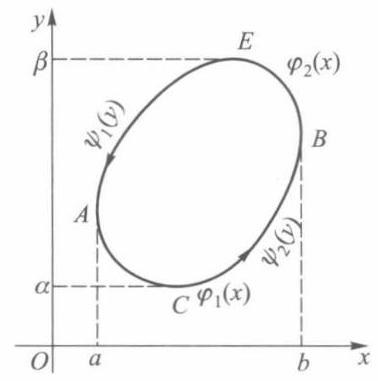
\includegraphics[width=.3\textwidth]{images/P166.jpg}
	\caption{图 $21-12$}
	\label{fig:P166}
\end{figure}

或
\[
{\psi }_{1}\left( y\right)  \leq  x \leq  {\psi }_{2}\left( y\right) ,\alpha  \leq  y \leq  \beta .
\]
这里 \(y = {\varphi }_{1}\left( x\right)\) 和 \(y = {\varphi }_{2}\left( x\right)\) 分别为曲线 \(\overset{⏜}{ACB}\) 和 \(\overset{⏜}{AEB}\) 的方程. 而 \(x = {\psi }_{1}\left( y\right)\) 和 \(x = {\psi }_{2}\left( y\right)\) 则分别是曲线 \(\overset{⏜}{CAE}\) 和 \(\overset{⏜}{CBE}\) 的方程. 于是
\[
{\iint }_{D}\frac{\partial Q}{\partial x}\mathrm{\;d}\sigma  = {\int }_{\alpha }^{\beta }\mathrm{d}y{\int }_{{\psi }_{1}\left( y\right) }^{{\psi }_{2}\left( y\right) }\frac{\partial Q}{\partial x}\mathrm{\;d}x
\]
\[
= {\int }_{\alpha }^{\beta }Q\left( {{\psi }_{2}\left( y\right) ,y}\right) \mathrm{d}y - {\int }_{\alpha }^{\beta }Q\left( {{\psi }_{1}\left( y\right) ,y}\right) \mathrm{d}y
\]
\[
= {\int }_{\overset{⏜}{CBE}}Q\left( {x,y}\right) \mathrm{d}y - {\int }_{\overset{⏜}{CAE}}Q\left( {x,y}\right) \mathrm{d}y
\]
\[
= {\int }_{\overset{⏜}{CBE}}Q\left( {x,y}\right) \mathrm{d}y + {\int }_{\overset{⏜}{EAC}}Q\left( {x,y}\right) \mathrm{d}y
\]
\[
= {\oint }_{L}Q\left( {x,y}\right) \mathrm{d}y\text{ . }
\]
同理可以证得
\[
- {\iint }_{D}\frac{\partial P}{\partial y}\mathrm{\;d}\sigma  = {\oint }_{L}P\left( {x,y}\right) \mathrm{d}x.
\]
将上述两个结果相加即得
\[
{\iint }_{D}\left( {\frac{\partial Q}{\partial x} - \frac{\partial P}{\partial y}}\right) \mathrm{d}\sigma  = {\oint }_{L}P\mathrm{\;d}x + Q\mathrm{\;d}y.
\]
(ii) 若区域 \(D\) 是由一条按段光滑的闭曲线围成,如图 21-13 所示,则先用几段光滑曲线将 \(D\) 分成有限个既是 \(x\) 型又是 \(y\) 型的子区域,然后逐块按 (i) 得到它们的格林公式, 并相加即可.

\begin{figure}
	\centering
	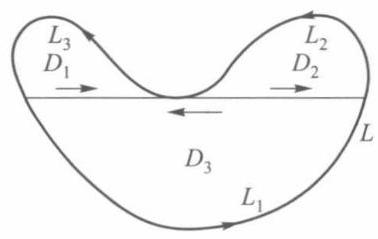
\includegraphics[width=.3\textwidth]{images/P167.jpg}
	\caption{图 $21-13$}
	\label{fig:P167}
\end{figure}

如图 21-13 所示的区域 \(D\) . 可将 \(D\) 分成三个既是 \(x\) 型又是 \(y\) 型的区域 \({D}_{1},{D}_{2},{D}_{3}\) . 于是
\[
{\iint }_{D}\left( {\frac{\partial Q}{\partial x} - \frac{\partial P}{\partial y}}\right) \mathrm{d}\sigma
\]
\[
= {\iint }_{{D}_{1}}\left( {\frac{\partial Q}{\partial x} - \frac{\partial P}{\partial y}}\right) \mathrm{d}\sigma  + {\iint }_{{D}_{2}}\left( {\frac{\partial Q}{\partial x} - \frac{\partial P}{\partial y}}\right) \mathrm{d}\sigma  + {\iint }_{{D}_{3}}\left( {\frac{\partial Q}{\partial x} - \frac{\partial P}{\partial y}}\right) \mathrm{d}\sigma
\]
\[
= {\oint }_{{L}_{1}}P\mathrm{\;d}x + Q\mathrm{\;d}y + {\oint }_{{L}_{2}}P\mathrm{\;d}x + Q\mathrm{\;d}y + {\oint }_{{L}_{3}}P\mathrm{\;d}x + Q\mathrm{\;d}y
\]
\[
= {\oint }_{L}P\mathrm{\;d}x + Q\mathrm{\;d}y\text{ . }
\]
(iii) 若区域 \(D\) 由几条闭曲线所围成,如图 21-14 所示,这时可适当添加直线段 \({AB},{CE}\) ,把区域转化为 (ii) 的情况来处理. 在图 21-14 中联结了 \({AB},{CE}\) 后,则 \(D\) 的边界曲线由 \({AB},{L}_{2},{BA},\overset{⏜}{AFC},{CE},{L}_{3},{EC}\) 及 \(\overset{⏜}{CGA}\) 构成. 由 (ii) 知
\[
{\iint }_{D}\left( {\frac{\partial Q}{\partial x} - \frac{\partial P}{\partial y}}\right) \mathrm{d}\sigma
\]
\[
= \left\{  {{\int }_{AB} + {\int }_{{L}_{2}} + {\int }_{BA} + {\int }_{\overset{⏜}{AFC}} + {\int }_{CE} + {\int }_{{L}_{3}} + {\int }_{EC} + {\int }_{\overset{⏜}{CGA}}}\right\}  \left( {P\mathrm{\;d}x + Q\mathrm{\;d}y}\right)
\]
\[
= \left( {{\oint }_{{L}_{2}} + {\oint }_{{L}_{3}} + {\oint }_{{L}_{1}}}\right) \left( {P\mathrm{\;d}x + Q\mathrm{\;d}y}\right)
\]
\[
= {\oint }_{L}P\mathrm{\;d}x + Q\mathrm{\;d}y\text{ . }
\]
格林公式沟通了沿闭曲线的积分与二重积分之间的联系. 为便于记忆, 格林公式 (1)也可写成下述形式:
\[
{\iint }_{D}\left| \begin{matrix} \frac{\partial }{\partial x} & \frac{\partial }{\partial y} \\  P & Q \end{matrix}\right| \mathrm{d}\sigma  = {\oint }_{L}P\mathrm{\;d}x + Q\mathrm{\;d}y.
\]
应用格林公式可以简化某些曲线积分的计算.

%例 1
\begin{example}

\end{example}
计算 \({\int }_{\overset{⏜}{AB}}x\mathrm{\;d}y\) ,其中曲线 \(\overset{⏜}{AB}\) 是半径为 \(r\) 的圆在第一象限部分 (图 21-15).

\begin{figure}
	\centering
	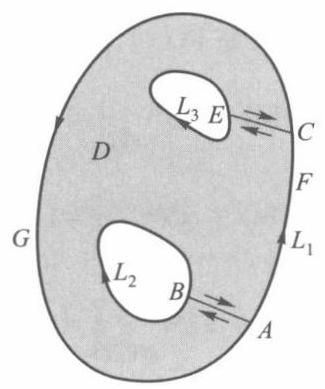
\includegraphics[width=.3\textwidth]{images/P168.jpg}
	\caption{图 $21-14$}
	\label{fig:P168}
\end{figure}

\begin{figure}
	\centering
	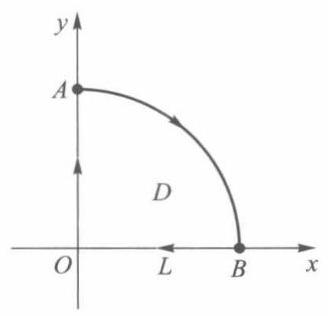
\includegraphics[width=.3\textwidth]{images/P169.jpg}
	\caption{图 $21-15$}
	\label{fig:P169}
\end{figure}

%解
\begin{solution}

\end{solution}
对半径为 \(r\) 的四分之一圆域 \(D\) ,应用格林公式有
\[
- {\iint }_{D}\mathrm{\;d}\sigma  = {\oint }_{-L}x\mathrm{\;d}y
\]
\[
= {\int }_{OA}x\mathrm{\;d}y + {\int }_{\overset{⏜}{AB}}x\mathrm{\;d}y + {\int }_{BO}x\mathrm{\;d}y.
\]
由于 \({\int }_{OA}x\mathrm{\;d}y = 0,{\int }_{BO}x\mathrm{\;d}y = 0\) ,所以
\[
{\int }_{\overset{⏜}{AB}}x\mathrm{\;d}y =  - {\iint }_{D}\mathrm{\;d}\sigma  =  - \frac{1}{4}\pi {r}^{2}.
\]
%例 2
\begin{example}

\end{example}
计算 \(I = {\oint }_{L}\frac{x\mathrm{\;d}y - y\mathrm{\;d}x}{{x}^{2} + {y}^{2}}\) ,其中 \(L\) 为任一不包含原点的闭区域的边界曲线,分段光滑.

%解
\begin{solution}

\end{solution}
因为
\[
\frac{\partial }{\partial x}\left( \frac{x}{{x}^{2} + {y}^{2}}\right)  = \frac{{y}^{2} - {x}^{2}}{{\left( {x}^{2} + {y}^{2}\right) }^{2}},\frac{\partial }{\partial y}\left( \frac{-y}{{x}^{2} + {y}^{2}}\right)  = \frac{{y}^{2} - {x}^{2}}{{\left( {x}^{2} + {y}^{2}\right) }^{2}}
\]
在上述区域 \(D\) 上连续且相等,于是
\[
{\iint }_{D}\left\lbrack  {\frac{\partial }{\partial x}\left( \frac{x}{{x}^{2} + {y}^{2}}\right)  - \frac{\partial }{\partial y}\left( \frac{-y}{{x}^{2} + {y}^{2}}\right) }\right\rbrack  \mathrm{d}\sigma  = 0,
\]
所以由格林公式立即可得
\[
I = 0\text{ . }
\]
在格林公式中,令 \(P =  - y,Q = x\) ,则得到一个计算平面区域 \(D\) 的面积 \({S}_{D}\) 的公式
\[
{S}_{D} = {\iint }_{D}\mathrm{\;d}\sigma  = \frac{1}{2}{\oint }_{L}x\mathrm{\;d}y - y\mathrm{\;d}x. \tag{2}
\]
%例 3
\begin{example}

\end{example}
计算抛物线 \({\left( x + y\right) }^{2} = {ax}\left( {a > 0}\right)\) 与 \(x\) 轴所围的面积 (图 21-16).

%解
\begin{solution}

\end{solution}
曲线 \(\overset{⏜}{AMO}\) 由函数 \(y = \sqrt{ax} - x,x \in  \left\lbrack  {0,a}\right\rbrack\) 表示, \(\overset{⏜}{ONA}\) 为直线 \(y = 0\) ,于是
\[
{S}_{D} = \frac{1}{2}\oint x\mathrm{\;d}y - y\mathrm{\;d}x
\]
\[
= \frac{1}{2}{\int }_{\overset{⏜}{ONA}}x\mathrm{\;d}y - y\mathrm{\;d}x + \frac{1}{2}{\int }_{\overset{⏜}{AMO}}x\mathrm{\;d}y - y\mathrm{\;d}x
\]
\[
= \frac{1}{2}{\int }_{\overset{⏜}{AMO}}x\mathrm{\;d}y - y\mathrm{\;d}x
\]
\[
= \frac{1}{2}{\int }_{a}^{0}\left\lbrack  {x\left( {\frac{a}{2\sqrt{ax}} - 1}\right)  - \left( {\sqrt{ax} - x}\right) }\right\rbrack  \mathrm{d}x
\]
\[
= \frac{1}{2}{\int }_{a}^{0} - \frac{1}{2}\sqrt{ax}\mathrm{\;d}x = \frac{\sqrt{a}}{4}{\int }_{0}^{a}\sqrt{x}\mathrm{\;d}x = \frac{1}{6}{a}^{2}.
\]
\begin{figure}
	\centering
	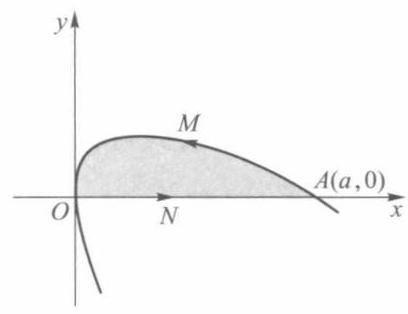
\includegraphics[width=.3\textwidth]{images/P170.jpg}
	\caption{图 $21-16$}
	\label{fig:P170}
\end{figure}

\subsection{曲线积分与路线的无关性}

在第二十章 §2 中计算第二型曲线积分的开始两个例子中,读者可能已经看到,在例 1 中,以 \(A\) 为起点 \(\text{ 、 }B\) 为终点的曲线积分,若所沿的路线不同,则其积分值也不同,但在例 2 中的曲线积分值只与起点和终点有关, 与路线的选取无关. 本段将讨论曲线积分在什么条件下, 它的值与所沿路线的选取无关.

首先,介绍单连通区域的概念.

若对于平面区域 \(D\) 上任一封闭曲线,皆可不经过 \(D\) 以外的点而连续收缩于属于 \(D\) 的某一点,则称此平面区域为单连通区域,否则称为复连通区域. 如图21-17中, \({D}_{1}\) 与

\({D}_{2}\) 是单连通区域,而 \({D}_{3}\) 与 \({D}_{4}\) 则是复连通区域. 单连通区域也可以这样叙述: \(D\) 内任一封闭曲线所围成的区域内只含有 \(D\) 中的点. 更通俗地说,单连通区域是没有 “洞” 的区域,复连通区域是有 “洞” 的区域.

\begin{figure}
	\centering
	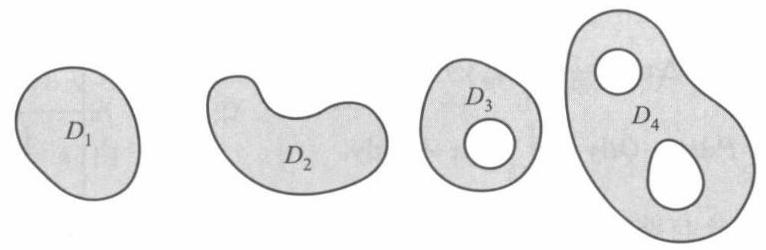
\includegraphics[width=.3\textwidth]{images/P171.jpg}
	\caption{图 $21-17$}
	\label{fig:P171}
\end{figure}

%定理 21.12
\begin{theorem}{}{the:}

\end{theorem}
 设 \(D\) 是单连通闭区域. 若函数 \(P\left( {x,y}\right) ,Q\left( {x,y}\right)\) 在 \(D\) 内连续,且具有一阶连续偏导数, 则以下四个条件等价:

(i) 沿 \(D\) 内任一按段光滑封闭曲线 \(L\) ,有
\[
{\oint }_{L}P\mathrm{\;d}x + Q\mathrm{\;d}y = 0;
\]
(ii) 对 \(D\) 中任一按段光滑曲线 \(L\) ,曲线积分
\[
{\int }_{L}P\mathrm{\;d}x + Q\mathrm{\;d}y
\]
与路线无关,只与 \(L\) 的起点及终点有关;

(iii) \(P\mathrm{\;d}x + Q\mathrm{\;d}y\) 是 \(D\) 内某一函数 \(u\left( {x,y}\right)\) 的全微分,即在 \(D\) 内有
\[
\mathrm{d}u = P\mathrm{\;d}x + Q\mathrm{\;d}y;
\]
(iv) 在 \(D\) 内处处成立
\[
\frac{\partial P}{\partial y} = \frac{\partial Q}{\partial x}.
\]
%证
\begin{proof}

\end{proof}
(i) \(\Rightarrow\) (ii) 如图 21-18,设 \(\overset{⏜}{ARB}\) 与 \(\overset{⏜}{ASB}\) 为联结点 \(A,B\) 的任意两条按段光滑曲线,由 (i) 可推得
\[
{\int }_{\overset{⏜}{ARB}}P\mathrm{\;d}x + Q\mathrm{\;d}y - {\int }_{\overset{⏜}{ASB}}P\mathrm{\;d}x + Q\mathrm{\;d}y
\]
\[
= {\int }_{\overset{⏜}{ARB}}P\mathrm{\;d}x + Q\mathrm{\;d}y + {\int }_{\overset{⏜}{BSA}}P\mathrm{\;d}x + Q\mathrm{\;d}y
\]
\[
= {\oint }_{\overset{⏜}{ARBSA}}P\mathrm{\;d}x + Q\mathrm{\;d}y = 0,
\]
\begin{figure}
	\centering
	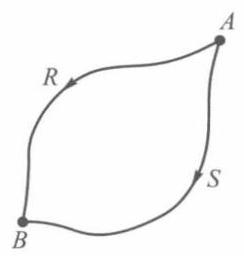
\includegraphics[width=.3\textwidth]{images/P172.jpg}
	\caption{图 $21-18$}
	\label{fig:P172}
\end{figure}

所以
\[
{\int }_{\overset{⏜}{ARB}}P\mathrm{\;d}x + Q\mathrm{\;d}y = {\int }_{\overset{⏜}{ASB}}P\mathrm{\;d}x + Q\mathrm{\;d}y.
\]
(ii) \(\Rightarrow\) (iii) 设 \(A\left( {{x}_{0},{y}_{0}}\right)\) 为 \(D\) 内某一定点, \(B\left( {x,y}\right)\) 为 \(D\) 内任意一点. 由 (ii),曲线积分
\[
{\int }_{\overset{⏜}{AB}}P\mathrm{\;d}x + Q\mathrm{\;d}y
\]
与路线的选择无关,故当 \(B\left( {x,y}\right)\) 在 \(D\) 内变动时,其积分值是 \(B\left( {x,y}\right)\) 的函数,即有
\[
u\left( {x,y}\right)  = {\int }_{\overset{⏜}{AB}}P\mathrm{\;d}x + Q\mathrm{\;d}y.
\]
取 \({\Delta x}\) 充分小,使 \(\left( {x + {\Delta x},y}\right)  \in  D\) ,则函数 \(u\left( {x,y}\right)\) 对于 \(x\) 的偏增量 (图 21-19)
\[
u\left( {x + {\Delta x},y}\right)  - u\left( {x,y}\right)
\]
\[
= {\int }_{\overset{⏜}{AC}}P\mathrm{\;d}x + Q\mathrm{\;d}y - {\int }_{\overset{⏜}{AB}}P\mathrm{\;d}x + Q\mathrm{\;d}y.
\]
\begin{figure}
	\centering
	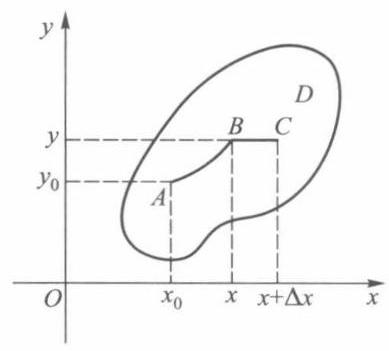
\includegraphics[width=.3\textwidth]{images/P173.jpg}
	\caption{图 $21-19$}
	\label{fig:P173}
\end{figure}

因为在 \(D\) 内曲线积分与路线无关,所以
\[
{\int }_{\overset{⏜}{AC}}P\mathrm{\;d}x + Q\mathrm{\;d}y
\]
\[
= {\int }_{\overset{⏜}{AB}}P\mathrm{\;d}x + Q\mathrm{\;d}y + {\int }_{BC}P\mathrm{\;d}x + Q\mathrm{\;d}y.
\]
由于直线段 \({BC}\) 平行于 \(x\) 轴,所以 \(\mathrm{d}y = 0\) ,从而由积分中值定理可得
\[
{\Delta u} = u\left( {x + {\Delta x},y}\right)  - u\left( {x,y}\right)  = {\int }_{BC}P\mathrm{\;d}x + Q\mathrm{\;d}y
\]
\[
= {\int }_{x}^{x + {\Delta x}}P\left( {s,y}\right) \mathrm{d}s = P\left( {x + {\theta \Delta x},y}\right) {\Delta x},
\]
其中 \(0 < \theta  < 1\) . 根据 \(P\left( {x,y}\right)\) 在 \(D\) 上连续,于是有
\[
\frac{\partial u}{\partial x} = \mathop{\lim }\limits_{{{\Delta x} \rightarrow  0}}\frac{\Delta u}{\Delta x} = \mathop{\lim }\limits_{{{\Delta x} \rightarrow  0}}P\left( {x + {\theta \Delta x},y}\right)  = P\left( {x,y}\right) .
\]
同理可证 \(\frac{\partial u}{\partial y} = Q\left( {x,y}\right)\) . 因此
\[
\mathrm{d}u = P\mathrm{\;d}x + Q\mathrm{\;d}y.
\]
\(\left( \text{ iii }\right)  \Rightarrow  \left( \text{ iv }\right)\) 设存在函数 \(u\left( {x,y}\right)\) ,使得
\[
\mathrm{d}u = P\mathrm{\;d}x + Q\mathrm{\;d}y,
\]
所以 \(P\left( {x,y}\right)  = \frac{\partial }{\partial x}u\left( {x,y}\right) ,Q\left( {x,y}\right)  = \frac{\partial }{\partial y}u\left( {x,y}\right)\) . 因此
\[
\frac{\partial P}{\partial y} = \frac{{\partial }^{2}u}{\partial x\partial y},\;\frac{\partial Q}{\partial x} = \frac{{\partial }^{2}u}{\partial y\partial x}.
\]
因为 \(P\left( {x,y}\right) ,Q\left( {x,y}\right)\) 在区域 \(D\) 内具有一阶连续偏导数,所以
\[
\frac{{\partial }^{2}u}{\partial x\partial y} = \frac{{\partial }^{2}u}{\partial y\partial x}.
\]
从而在 \(D\) 内每一点处都有
\[
\frac{\partial P}{\partial y} = \frac{\partial Q}{\partial x}.
\]
(iv) \(\Rightarrow\) (i) 设 \(L\) 为 \(D\) 内任一按段光滑封闭曲线,记 \(L\) 所围的区域为 \(\sigma\) . 由于 \(D\) 为单连通区域,所以区域 \(\sigma\) 含在 \(D\) 内. 应用格林公式及在 \(D\) 内恒有 \(\frac{\partial P}{\partial y} = \frac{\partial Q}{\partial x}\) 的条件,就得到
\[
{\oint }_{L}P\mathrm{\;d}x + Q\mathrm{\;d}y = {\iint }_{\sigma }\left( {\frac{\partial Q}{\partial x} - \frac{\partial P}{\partial y}}\right) \mathrm{d}\sigma  = 0.
\]
上面我们将四个条件循环推导了一遍, 这就证明了它们是相互等价的.

应用定理 21.12 中的条件 (iv) 考察第二十章 §2 中的例 1 与例 2 . 在例 1 中 \(P\left( {x,y}\right)  = {xy},Q\left( {x,y}\right)  = y - x\) . 由于 \(\frac{\partial P}{\partial y} = x,\frac{\partial Q}{\partial x} =  - 1,\frac{\partial P}{\partial y} \neq  \frac{\partial Q}{\partial x}\) ,故积分与路线有关. 在例 2 中 \(P\left( {x,y}\right)  = y,Q\left( {x,y}\right)  = x\) ,由于
\[
\frac{\partial P}{\partial y} = \frac{\partial Q}{\partial x} = 1,
\]
所以积分与路线无关.

%定理 21.12
\begin{theorem}{}{the:}

\end{theorem}
 中要求 \(D\) 为单连通区域是重要的. 如本节例 2,对任何不包含原点的单连通区域 \(D\) ,已证得在这个 \(D\) 内的任何封闭曲线 \(L\) 上,皆有
\[
{\oint }_{L}\frac{x\mathrm{\;d}y - y\mathrm{\;d}x}{{x}^{2} + {y}^{2}} = 0. \tag{3}
\]
倘若 \(L\) 为绕原点一周的封闭曲线,则函数 \(P\left( {x,y}\right)  = \frac{-y}{{x}^{2} + {y}^{2}},Q\left( {x,y}\right)  = \frac{x}{{x}^{2} + {y}^{2}}\) 只在剔除原点外的任何区域 \(D\) 上有定义,所以 \(L\) 必含在某个复连通区域内. 这时它不满足定理 21.12的条件,因而就不能保证 (3) 式成立. 事实上,设 \(L\) 为绕原点一周的圆
\[
L : x = a\cos \theta ,y = a\sin \theta \;\left( {0 \leq  \theta  \leq  {2\pi }}\right) ,
\]
则有
\[
{\oint }_{L}\frac{x\mathrm{\;d}y - y\mathrm{\;d}x}{{x}^{2} + {y}^{2}} = {\int }_{0}^{2\pi }\frac{{a}^{2}{\cos }^{2}\theta  + {a}^{2}{\sin }^{2}\theta }{{a}^{2}}\mathrm{\;d}\theta  = {\int }_{0}^{2\pi }\mathrm{d}\theta  = {2\pi }.
\]
若 \(P\left( {x,y}\right) ,Q\left( {x,y}\right)\) 满足定理 21.12 的条件,则由上述证明可看到二元函数
\[
u\left( {x,y}\right)  = {\int }_{\overset{⏜}{AB}}P\left( {x,y}\right) \mathrm{d}x + Q\left( {x,y}\right) \mathrm{d}y
\]
\[
= {\int }_{A\left( {{x}_{0},{y}_{0}}\right) }^{B\left( {x,y}\right) }P\left( {s,t}\right) \mathrm{d}s + Q\left( {s,t}\right) \mathrm{d}t
\]
具有性质
\[
\mathrm{d}u\left( {x,y}\right)  = P\left( {x,y}\right) \mathrm{d}x + Q\left( {x,y}\right) \mathrm{d}y.
\]
它与一元函数的原函数相仿. 所以我们也称 \(u\left( {x,y}\right)\) 为 \(P\mathrm{\;d}x + Q\mathrm{\;d}y\) 的一个原函数.

设 \(I,J\) 是区间, \(P\left( {x,y}\right) ,Q\left( {x,y}\right)\) 在 \(D = I \times  J\) 上有连续偏导数,且 \(\frac{\partial P}{\partial y} = \frac{\partial Q}{\partial x}\) 处处成立,则任取定 \(\left( {{x}_{0},{y}_{0}}\right)  \in  D\) ,对于 \(\left( {x,y}\right)  \in  D\) ,取路线为图 21-20 中的折线 \({ABC}\) ,由定理 21.12,
\[
u\left( {x,y}\right)  = {\int }_{{x}_{0}}^{x}P\left( {s,{y}_{0}}\right) \mathrm{d}s + {\int }_{{y}_{0}}^{y}Q\left( {x,t}\right) \mathrm{d}t
\]
\begin{figure}
	\centering
	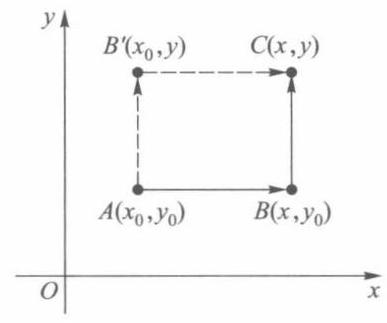
\includegraphics[width=.3\textwidth]{images/P174.jpg}
	\caption{图 $21-20$}
	\label{fig:P174}
\end{figure}

是 \(P\left( {x,y}\right) \mathrm{d}x + Q\left( {x,y}\right) \mathrm{d}y\) 的一个原函数. 同理,取路线 \(A{B}^{\prime }C\) ,


\[
u\left( {x,y}\right)  = {\int }_{{x}_{0}}^{x}P\left( {s,y}\right) \mathrm{d}s + {\int }_{{y}_{0}}^{y}Q\left( {{x}_{0},t}\right) \mathrm{d}t
\]
\begin{center}

\includegraphics[width=.3\textwidth]{images/P175.jpg}
\end{center}


也是 \(P\left( {x,y}\right) \mathrm{d}x + Q\left( {x,y}\right) \mathrm{d}y\) 的一个原函数.

%例 4
\begin{example}

\end{example}
试用曲线积分求
\[
\left( {{2x} + \sin y}\right) \mathrm{d}x + \left( {x\cos y}\right) \mathrm{d}y
\]
的一个原函数.

%解
\begin{solution}

\end{solution}
由于 \(\frac{\partial }{\partial y}\left( {{2x} + \sin y}\right)  = \cos y = \frac{\partial }{\partial x}\left( {x\cos y}\right)\) ,因此可取 \(\left( {{x}_{0},{y}_{0}}\right)  = \left( {0,0}\right)\) ,有
\[
u\left( {x,y}\right)  = {\int }_{0}^{x}{2s}\mathrm{\;d}s + {\int }_{0}^{y}x\cos t\mathrm{\;d}t = {x}^{2} + x\sin y.
\]
\subsection{习题 21.3}

1. 应用格林公式计算下列曲线积分:

(1) \({\oint }_{L}{\left( x + y\right) }^{2}\mathrm{\;d}x - \left( {{x}^{2} + {y}^{2}}\right) \mathrm{d}y\) ,其中 \(L\) 是以 \(A\left( {1,1}\right) ,B\left( {3,2}\right) ,C\left( {2,5}\right)\) 为顶点的三角形,方向取正向;

(2) \({\int }_{AB}\left( {{\mathrm{e}}^{x}\sin y - {my}}\right) \mathrm{d}x + \left( {{\mathrm{e}}^{x}\cos y - m}\right) \mathrm{d}y\) ,其中 \(m\) 为常数, \({AB}\) 为由(a,0)到(0,0)经过圆 \({x}^{2} + {y}^{2} =\)  \({ax}\) 上半部的路线 \(\left( {a > 0}\right)\) .

2. 应用格林公式计算下列曲线所围的平面面积:

(1)星形线: \(x = a{\cos }^{3}t,y = a{\sin }^{3}t\) ；

(2) 双纽线: \({\left( {x}^{2} + {y}^{2}\right) }^{2} = {a}^{2}\left( {{x}^{2} - {y}^{2}}\right)\) .

3. 证明: 若 \(L\) 为平面上封闭曲线, \(l\) 为任意方向向量,则
\[
{\oint }_{L}\cos \left( {\overset{⏜}{\mathbf{l}},\mathbf{n}}\right) \mathrm{d}s = 0,
\]
其中 \(\mathbf{n}\) 为曲线 \(L\) 的外法线方向.

4. 求积分值 \(I = {\oint }_{L}\left\lbrack  {x\cos \left( \overset{⏜}{n,x}\right)  + y\cos \left( \overset{⏜}{n,y}\right) }\right\rbrack  \mathrm{d}s\) ,其中 \(L\) 为包围有界区域的封闭曲线, \(n\) 为 \(L\) 的外法线方向.

5. 验证下列积分与路线无关, 并求它们的值:

(1) \({\int }_{\left( 0,0\right) }^{\left( 1,1\right) }\left( {x - y}\right) \left( {\mathrm{d}x - \mathrm{d}y}\right)\) ;

(2) \({\int }_{\left( 0,0\right) }^{\left( x,y\right) }\left( {{2x}\cos y - {y}^{2}\sin x}\right) \mathrm{d}x + \left( {{2y}\cos x - {x}^{2}\sin y}\right) \mathrm{d}y\) ;

(3) \({\int }_{\left( 2,1\right) }^{\left( 1,2\right) }\frac{y\mathrm{\;d}x - x\mathrm{\;d}y}{{x}^{2}}\) ,沿在右半平面的路线；

(4) \({\int }_{\left( 1,0\right) }^{\left( 6,8\right) }\frac{x\mathrm{\;d}x + y\mathrm{\;d}y}{\sqrt{{x}^{2} + {y}^{2}}}\) ,沿不通过原点的路线；

(5) \({\int }_{\left( 2,1\right) }^{\left( 1,2\right) }\varphi \left( x\right) \mathrm{d}x + \psi \left( y\right) \mathrm{d}y\) ,其中 \(\varphi \left( x\right) ,\psi \left( y\right)\) 为连续函数.

6. 求下列全微分的原函数:

(1) \(\left( {{x}^{2} + {2xy} - {y}^{2}}\right) \mathrm{d}x + \left( {{x}^{2} - {2xy} - {y}^{2}}\right) \mathrm{d}y\) ;

(2) \({\mathrm{e}}^{x}\left\lbrack  {{\mathrm{e}}^{y}\left( {x - y + 2}\right)  + y}\right\rbrack  \mathrm{d}x + {\mathrm{e}}^{x}\left\lbrack  {{\mathrm{e}}^{y}\left( {x - y}\right)  + 1}\right\rbrack  \mathrm{d}y\) ;

(3) \(f\left( \sqrt{{x}^{2} + {y}^{2}}\right) x\mathrm{\;d}x + f\left( \sqrt{{x}^{2} + {y}^{2}}\right) y\mathrm{\;d}y\) .

7. 为了使曲线积分
\[
{\int }_{L}F\left( {x,y}\right) \left( {y\mathrm{\;d}x + x\mathrm{\;d}y}\right)
\]
与积分路线无关,可微函数 \(F\left( {x,y}\right)\) 应满足怎样的条件?

8. 计算曲线积分
\[
{\int }_{\overset{⏜}{AMB}}\left\lbrack  {\varphi \left( y\right) {\mathrm{e}}^{x} - {my}}\right\rbrack  \mathrm{d}x + \left\lbrack  {{\varphi }^{\prime }\left( y\right) {\mathrm{e}}^{x} - m}\right\rbrack  \mathrm{d}y,
\]
其中 \(\varphi \left( y\right)\) 和 \({\varphi }^{\prime }\left( y\right)\) 为连续函数, \(\overset{⏜}{AMB}\) 为连接点 \(A\left( {{x}_{1},{y}_{1}}\right)\) 和点 \(B\left( {{x}_{2},{y}_{2}}\right)\) 的任何路线,但与直线段 \({AB}\) 围成已知大小为 \(S\) 的面积.

9. 设函数 \(f\left( u\right)\) 具有一阶连续导数,证明对任何光滑封闭曲线 \(L\) ,有
\[
{\oint }_{L}f\left( {xy}\right) \left( {y\mathrm{\;d}x + x\mathrm{\;d}y}\right)  = 0.
\]
10. 设函数 \(u\left( {x,y}\right)\) 在由封闭的光滑曲线 \(L\) 所围的区域 \(D\) 上具有二阶连续偏导数,证明
\[
{\iint }_{D}\left( {\frac{{\partial }^{2}u}{\partial {x}^{2}} + \frac{{\partial }^{2}u}{\partial {y}^{2}}}\right) \mathrm{d}\sigma  = {\oint }_{L}\frac{\partial u}{\partial \mathbf{n}}\mathrm{d}s,
\]
其中 \(\frac{\partial u}{\partial \mathbf{n}}\) 是 \(u\left( {x,y}\right)\) 沿 \(L\) 外法线方向 \(\mathbf{n}\) 的方向导数.

\section{二重积分的变量变换}

\subsection{二重积分的变量变换公式}

在定积分的计算中,我们得到了如下结论: 设 \(f\left( x\right)\) 在区间 \(\left\lbrack  {a,b}\right\rbrack\) 上连续, \(x = \varphi \left( t\right)\) 当 \(t\) 从 \(\alpha\) 变到 \(\beta\) 时,严格单调地从 \(a\) 变到 \(b\) ,且 \(\varphi \left( t\right)\) 连续可微,则
\[
{\int }_{a}^{b}f\left( x\right) \mathrm{d}x = {\int }_{\alpha }^{\beta }f\left( {\varphi \left( t\right) }\right) {\varphi }^{\prime }\left( t\right) \mathrm{d}t. \tag{1}
\]
当 \(\alpha  < \beta\) (即 \({\varphi }^{\prime }\left( t\right)  > 0\) ) 时,记 \(X = \left\lbrack  {a,b}\right\rbrack  ,Y = \left\lbrack  {\alpha ,\beta }\right\rbrack\) ,则 \(X = \varphi \left( Y\right) ,Y = {\varphi }^{-1}\left( X\right)\) . 利用这些记号,公式 (1) 又可写成
\[
{\int }_{X}f\left( x\right) \mathrm{d}x = {\int }_{{\varphi }^{-1}\left( X\right) }f\left( {\varphi \left( t\right) }\right) {\varphi }^{\prime }\left( t\right) \mathrm{d}t. \tag{2}
\]
当 \(\alpha  > \beta\) (即 \({\varphi }^{\prime }\left( t\right)  < 0\) ) 时,(1) 式可写成
\[
{\int }_{X}f\left( x\right) \mathrm{d}x =  - {\int }_{{\varphi }^{-1}\left( X\right) }f\left( {\varphi \left( t\right) }\right) {\varphi }^{\prime }\left( t\right) \mathrm{d}t. \tag{3}
\]
故当 \(\varphi \left( t\right)\) 为严格单调且连续可微时,(2)式和(3)式可统一写成如下的形式:
\[
{\int }_{X}f\left( x\right) \mathrm{d}x = {\int }_{{\varphi }^{-1}\left( X\right) }f\left( {\varphi \left( t\right) }\right) \left| {{\varphi }^{\prime }\left( t\right) }\right| \mathrm{d}t. \tag{4}
\]
下面我们把公式 (4) 推广到二重积分的场合. 为此, 先给出下面的引理.

引理 设变换 \(T : x = x\left( {u,v}\right) ,y = y\left( {u,v}\right)\) 将 \({uv}\) 平面上由按段光滑封闭曲线所围的闭区域 \(\Delta\) 一对一地映成 \({xy}\) 平面上的闭区域 \(D\) ,函数 \(x\left( {u,v}\right) ,y\left( {u,v}\right)\) 在 \(\Delta\) 内分别具有一阶连续偏导数且它们的函数行列式
\[
J\left( {u,v}\right)  = \frac{\partial \left( {x,y}\right) }{\partial \left( {u,v}\right) } \neq  0,\;\left( {u,v}\right)  \in  \Delta ,
\]
则区域 \(D\) 的面积
\[
\mu \left( D\right)  = {\iint }_{\Delta }\left| {J\left( {u,v}\right) }\right| \mathrm{d}u\mathrm{\;d}v. \tag{5}
\]
%证
\begin{proof}

\end{proof}
下面给出当 \(y\left( {u,v}\right)\) 在 \(\Delta\) 内具有二阶连续偏导数时的证明. 对 \(y\left( {u,v}\right)\) 具有一阶连续偏导数条件下的证明在本章 §9 中给出.

由于 \(T\) 是一对一变换,且 \(J\left( {u,v}\right)  \neq  0\) ,因而 \(T\) 把 \(\Delta\) 的内点变为 \(D\) 的内点,所以 \(\Delta\) 的按段光滑边界曲线 \({L}_{\Delta }\) 变换到 \(D\) 时,其边界曲线 \({L}_{D}\) 也是按段光滑的.

设曲线 \({L}_{\Delta }\) 的参数方程为
\[
u = u\left( t\right) ,\;v = v\left( t\right) \;\left( {\alpha  \leq  t \leq  \beta }\right) .
\]
由于 \({L}_{\Delta }\) 按段光滑,所以 \({u}^{\prime }\left( t\right) ,{v}^{\prime }\left( t\right)\) 在 \(\left\lbrack  {\alpha ,\beta }\right\rbrack\) 上至多除去有限个第一类间断点外,在其他的点上都连续. 因为 \({L}_{D} = T\left( {L}_{\Delta }\right)\) ,所以 \({L}_{D}\) 的参数方程为
\[
\begin{array}{l} x = x\left( t\right)  = x\left( {u\left( t\right) ,v\left( t\right) }\right) ,\;\left( {\alpha  \leq  t \leq  \beta }\right) . \\  y = y\left( t\right)  = y\left( {u\left( t\right) ,v\left( t\right) }\right)  \end{array}
\]
若规定 \(t\) 从 \(\alpha\) 变到 \(\beta\) 时,对应于 \({L}_{D}\) 的正向,则根据格林公式,取 \(P\left( {x,y}\right)  = 0\) , \(Q\left( {x,y}\right)  = x\) ,有
\[
\mu \left( D\right)  = {\oint }_{{L}_{D}}x\mathrm{\;d}y = {\int }_{\alpha }^{\beta }x\left( t\right) {y}^{\prime }\left( t\right) \mathrm{d}t
\]
\[
= {\int }_{\alpha }^{\beta }x\left( {u\left( t\right) ,v\left( t\right) }\right) \left\lbrack  {\frac{\partial y}{\partial u}{u}^{\prime }\left( t\right)  + \frac{\partial y}{\partial v}{v}^{\prime }\left( t\right) }\right\rbrack  \mathrm{d}t. \tag{6}
\]
另一方面,在 \({uv}\) 平面上
\[
{\oint }_{{L}_{\Delta }}x\left( {u,v}\right) \left\lbrack  {\frac{\partial y}{\partial u}\mathrm{\;d}u + \frac{\partial y}{\partial v}\mathrm{\;d}v}\right\rbrack
\]
\[
=  \pm  {\int }_{\alpha }^{\beta }x\left( {u\left( t\right) ,v\left( t\right) }\right) \left\lbrack  {\frac{\partial y}{\partial u}{u}^{\prime }\left( t\right)  + \frac{\partial y}{\partial v}{v}^{\prime }\left( t\right) }\right\rbrack  \mathrm{d}t, \tag{7}
\]
其中正号及负号分别由 \(t\) 从 \(\alpha\) 变到 \(\beta\) 时,是对应于 \({L}_{\Delta }\) 的正方向或负方向所决定. 由 (6)及(7)式得到
\[
\mu \left( D\right)  =  \pm  {\oint }_{{L}_{\Delta }}x\left( {u,v}\right) \left\lbrack  {\frac{\partial y}{\partial u}\mathrm{\;d}u + \frac{\partial y}{\partial v}\mathrm{\;d}v}\right\rbrack
\]
\[
=  \pm  {\oint }_{{L}_{\Delta }}x\left( {u,v}\right) \frac{\partial y}{\partial u}\mathrm{\;d}u + x\left( {u,v}\right) \frac{\partial y}{\partial v}\mathrm{\;d}v.
\]
令 \(P\left( {u,v}\right)  = x\left( {u,v}\right) \frac{\partial y}{\partial u},Q\left( {u,v}\right)  = x\left( {u,v}\right) \frac{\partial y}{\partial v}\) ,在 \({uv}\) 平面上对上式应用格林公式,得到
\[
\mu \left( D\right)  =  \pm  {\iint }_{\Delta }\left( {\frac{\partial Q}{\partial u} - \frac{\partial P}{\partial v}}\right) \mathrm{d}u\mathrm{\;d}v.
\]
由于函数 \(y\left( {u,v}\right)\) 具有二阶连续偏导数,即有 \(\frac{{\partial }^{2}y}{\partial u\partial v} = \frac{{\partial }^{2}y}{\partial v\partial u}\) ,因此, \(\frac{\partial Q}{\partial u} - \frac{\partial P}{\partial v} = J\left( {u,v}\right)\) ,于是
\[
\mu \left( D\right)  =  \pm  {\iint }_{\Delta }J\left( {u,v}\right) \mathrm{d}u\mathrm{\;d}v.
\]
又因为 \(\mu \left( D\right)\) 总是非负的,而 \(J\left( {u,v}\right)\) 在 \(\Delta\) 上不为零且连续,故其函数值在 \(\Delta\) 上不变号, 所以
\[
\mu \left( D\right)  = {\iint }_{\Delta }\left| {J\left( {u,v}\right) }\right| \mathrm{d}u\mathrm{\;d}v.
\]
%定理 21.13
\begin{theorem}{}{the:}

\end{theorem}
 设 \(f\left( {x,y}\right)\) 在有界闭区域 \(D\) 上可积,变换 \(T : x = x\left( {u,v}\right) ,y = y\left( {u,v}\right)\) 将 \({uv}\) 平面由按段光滑封闭曲线所围成的闭区域 \(\Delta\) 一对一地映成 \({xy}\) 平面上的闭区域 \(D\) , 函数 \(x\left( {u,v}\right) ,y\left( {u,v}\right)\) 在 \(\Delta\) 内分别具有一阶连续偏导数且它们的函数行列式
\[
J\left( {u,v}\right)  = \frac{\partial \left( {x,y}\right) }{\partial \left( {u,v}\right) } \neq  0,\;\left( {u,v}\right)  \in  \Delta ,
\]
则
\[
{\iint }_{D}f\left( {x,y}\right) \mathrm{d}x\mathrm{\;d}y = {\iint }_{\Delta }f\left( {x\left( {u,v}\right) ,y\left( {u,v}\right) }\right) \left| {J\left( {u,v}\right) }\right| \mathrm{d}u\mathrm{\;d}v.
\]
%证
\begin{proof}

\end{proof}
用曲线网把 \(\Delta\) 分成 \(n\) 个小区域 \({\Delta }_{i}\) ,在变换 \(T\) 作用下,区域 \(D\) 也相应地被分成 \(n\) 个小区域 \({D}_{i}\) . 记 \({\Delta }_{i}\) 及 \({D}_{i}\) 的面积为 \(\mu \left( {\Delta }_{i}\right)\) 及 \(\mu \left( {D}_{i}\right) \left( {i = 1,2,\cdots ,n}\right)\) . 由引理及二重积分中值定理, 有
\[
\mu \left( {D}_{i}\right)  = {\iint }_{{\Delta }_{i}}\left| {J\left( {u,v}\right) }\right| \mathrm{d}u\mathrm{\;d}v = \left| {J\left( {{\bar{u}}_{i},{\bar{v}}_{i}}\right) }\right| \mu \left( {\Delta }_{i}\right) ,
\]
其中 \(\left( {{\bar{u}}_{i},{\bar{v}}_{i}}\right)  \in  {\Delta }_{i}\left( {i = 1,2,\cdots ,n}\right)\) .

令 \({\xi }_{i} = x\left( {{\bar{u}}_{i},{\bar{v}}_{i}}\right) ,{\eta }_{i} = y\left( {{\bar{u}}_{i},{\bar{v}}_{i}}\right)\) ,则 \(\left( {{\xi }_{i},{\eta }_{i}}\right)  \in  {D}_{i}\left( {i = 1,2,\cdots ,n}\right)\) . 作二重积分 \({\iint }_{D}f\left( {x,y}\right) \mathrm{d}x\mathrm{\;d}y\) 的积分和
\[
\sigma  = \mathop{\sum }\limits_{{i = 1}}^{n}f\left( {{\xi }_{i},{\eta }_{i}}\right) \mu \left( {D}_{i}\right)
\]
\[
= \mathop{\sum }\limits_{{i = 1}}^{n}f\left( {x\left( {{\bar{u}}_{i},{\bar{v}}_{i}}\right) ,y\left( {{\bar{u}}_{i},{\bar{v}}_{i}}\right) }\right) \left| {J\left( {{\bar{u}}_{i},{\bar{v}}_{i}}\right) }\right| \mu \left( {\Delta }_{i}\right) .
\]
上式右边的和式是 \(\Delta\) 上可积函数 \(f\left( {x\left( {u,v}\right) ,y\left( {u,v}\right) }\right) \left| {J\left( {u,v}\right) }\right|\) 的积分和. 又由变换 \(T\) 的连续性可知,当区域 \(\Delta\) 的分割 \({T}_{\Delta } : \left\{  {{\Delta }_{1},{\Delta }_{2},\cdots ,{\Delta }_{n}}\right\}\) 的细度 \(\begin{Vmatrix}{T}_{\Delta }\end{Vmatrix} \rightarrow  0\) 时,区域 \(D\) 相应的分割 \({T}_{D} : \left\{  {{D}_{1},{D}_{2},\cdots ,{D}_{n}}\right\}\) 的细度 \(\begin{Vmatrix}{T}_{D}\end{Vmatrix}\) 也趋于零. 因此得到
\[
{\iint }_{D}f\left( {x,y}\right) \mathrm{d}x\mathrm{\;d}y = {\iint }_{\Delta }f\left( {x\left( {u,v}\right) ,y\left( {u,v}\right) }\right) \left| {J\left( {u,v}\right) }\right| \mathrm{d}u\mathrm{\;d}v.
\]
%例 1
\begin{example}

\end{example}
求 \({\iint }_{D}{\mathrm{e}}^{\frac{x - y}{x + y}}\mathrm{\;d}x\mathrm{\;d}y\) ,其中 \(D\) 是由 \(x = 0,y = 0,x + y = 1\) 所围区域 (图 21-21).

%解
\begin{solution}

\end{solution}
为了简化被积函数,令 \(u = x - y,v = x + y\) . 为此作变换 \(T : x = \frac{1}{2}\left( {u + v}\right)\) , \(y = \frac{1}{2}\left( {v - u}\right)\) ,则
\[
J\left( {u,v}\right)  = \left| \begin{matrix} \frac{1}{2} & \frac{1}{2} \\   - \frac{1}{2} & \frac{1}{2} \end{matrix}\right|  = \frac{1}{2} > 0.
\]
在变换 \(T\) 的作用下,区域 \(D\) 的原象 \(\Delta\) 如图 21-22 所示. 所以
\[
{\iint }_{D}{\mathrm{e}}^{\frac{x - y}{x + y}}\mathrm{\;d}x\mathrm{\;d}y = {\iint }_{\Delta }{\mathrm{e}}^{\frac{u}{v}} \cdot  \frac{1}{2}\mathrm{\;d}u\mathrm{\;d}v = \frac{1}{2}{\int }_{0}^{1}\mathrm{\;d}v{\int }_{-v}^{v}{\mathrm{e}}^{\frac{u}{v}}\mathrm{\;d}u
\]
\[
= \frac{1}{2}{\int }_{0}^{1}v\left( {\mathrm{e} - {\mathrm{e}}^{-1}}\right) \mathrm{d}v = \frac{\mathrm{e} - {\mathrm{e}}^{-1}}{4}.
\]
\begin{figure}
	\centering
	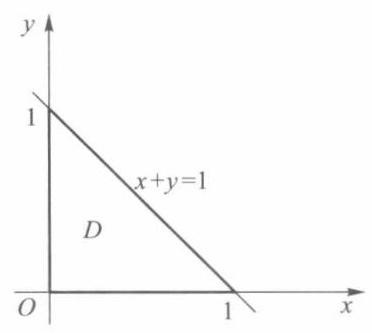
\includegraphics[width=.3\textwidth]{images/P176.jpg}
	\caption{图 $21-21$}
	\label{fig:P176}
\end{figure}

\begin{figure}
	\centering
	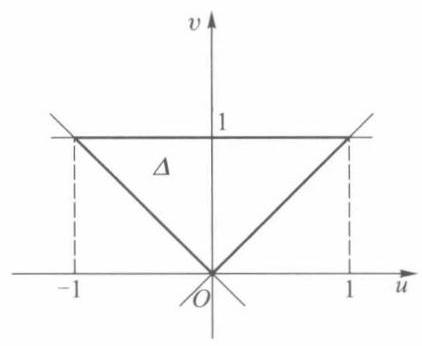
\includegraphics[width=.3\textwidth]{images/P177.jpg}
	\caption{图 $21-22$}
	\label{fig:P177}
\end{figure}

%例 2
\begin{example}

\end{example}
求抛物线 \({y}^{2} = {mx},{y}^{2} = {nx}\) 和直线 \(y = {\alpha x},y = {\beta x}\) 所围区域 \(D\) 的面积 \(\mu \left( D\right) \;\left( {0 < m < n,0 < \alpha  < \beta }\right) .\)

%解
\begin{solution}

\end{solution}
\(D\) 的面积
\[
\mu \left( D\right)  = {\iint }_{D}\mathrm{\;d}x\mathrm{\;d}y.
\]
\begin{figure}
	\centering
	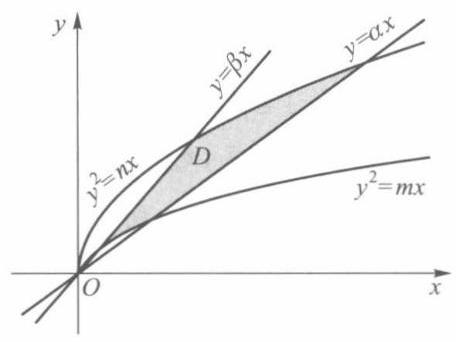
\includegraphics[width=.3\textwidth]{images/P178.jpg}
	\caption{图 $21-23$}
	\label{fig:P178}
\end{figure}

为了简化积分区域, 作变换
\[
x = \frac{u}{{v}^{2}},\;y = \frac{u}{v}.
\]
它把 \({xy}\) 平面上的区域 \(D\) (图 21-23 中的阴影部分) 对应到 \({uv}\) 平面上的矩形区域 \(\Delta  = \left\lbrack  {m,n}\right\rbrack   \times  \left\lbrack  {\alpha ,\beta }\right\rbrack\) . 由于
\[
J\left( {u,v}\right)  = \left| \begin{matrix} \frac{1}{{v}^{2}} &  - \frac{2u}{{v}^{3}} \\  \frac{1}{v} &  - \frac{u}{{v}^{2}} \end{matrix}\right|  = \frac{u}{{v}^{4}} > 0,\;\left( {u,v}\right)  \in  \Delta ,
\]
所以
\[
\mu \left( D\right)  = {\iint }_{D}\mathrm{\;d}\sigma  = {\iint }_{\Delta }\frac{u}{{v}^{4}}\mathrm{\;d}u\mathrm{\;d}v
\]
\[
= {\int }_{\alpha }^{\beta }\frac{\mathrm{d}v}{{v}^{4}} \cdot  {\int }_{m}^{n}u\mathrm{\;d}u = \frac{\left( {{n}^{2} - {m}^{2}}\right) \left( {{\beta }^{3} - {\alpha }^{3}}\right) }{6{\alpha }^{3}{\beta }^{3}}.
\]
\subsection{用极坐标计算二重积分}

当积分区域是圆域或圆域的一部分,或者被积函数的形式为 \(f\left( {{x}^{2} + {y}^{2}}\right)\) 时,采用极坐标变换
\[
T : \left\{  {\begin{array}{l} x = r\cos \theta , \\  y = r\sin \theta , \end{array}\;0 \leq  r <  + \infty ,0 \leq  \theta  \leq  {2\pi }}\right.  \tag{8}
\]
往往能达到简化积分区域或被积函数的目的. 此时,变换 \(T\) 的函数行列式为
\[
J\left( {r,\theta }\right)  = \left| \begin{array}{rr} \cos \theta &  - r\sin \theta \\  \sin \theta & r\cos \theta  \end{array}\right|  = r.
\]
容易知道,极坐标变换 \(T\) 把 \({r\theta }\) 平面上的矩形 \(\left\lbrack  {0,R}\right\rbrack   \times  \left\lbrack  {0,{2\pi }}\right\rbrack\) 变换成 \({xy}\) 平面上的圆域 \(D = \left\{  {\left( {x,y}\right)  \mid  {x}^{2} + {y}^{2} \leq  {R}^{2}}\right\}\) . 但对应不是一对一的. 例如, \({xy}\) 平面上原点 \(O\left( {0,0}\right)\) 与 \({r\theta }\) 平面上直线 \(r = 0\) 相对应, \(x\) 轴上线段 \(A{A}^{\prime }\) 对应于 \({r\theta }\) 平面上两条线段 \({CD}\) 和 \({EF}\) (图 21-24). 又当 \(r = 0\) 时, \(J\left( {r,\theta }\right)  = 0\) ,因此不满足定理 21.13 的条件. 但是,我们仍然有下面的结论.

\begin{figure}
	\centering
	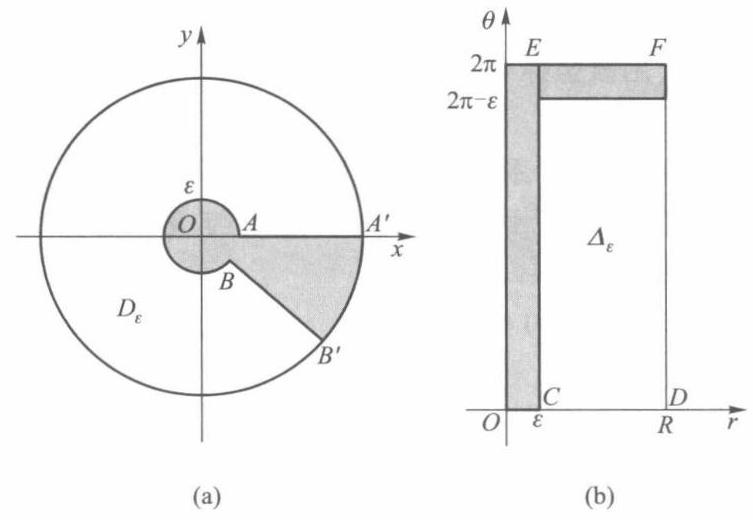
\includegraphics[width=.3\textwidth]{images/P179.jpg}
	\caption{图 $21-24$}
	\label{fig:P179}
\end{figure}

%定理 21.14
\begin{theorem}{}{the:}

\end{theorem}
 设 \(f\left( {x,y}\right)\) 满足定理 21.13 的条件,且在极坐标变换 (8) 下, \({xy}\) 平面上有界闭区域 \(D\) 与 \({r\theta }\) 平面上区域 \(\Delta\) 对应,则成立
\[
{\iint }_{D}f\left( {x,y}\right) \mathrm{d}x\mathrm{\;d}y = {\iint }_{\Delta }f\left( {r\cos \theta ,r\sin \theta }\right) r\mathrm{\;d}r\mathrm{\;d}\theta . \tag{9}
\]
%证
\begin{proof}

\end{proof}
若 \(D\) 为圆域 \(\left\{  {\left( {x,y}\right)  \mid  {x}^{2} + {y}^{2} \leq  {R}^{2}}\right\}\) ,则 \(\Delta\) 为 \({r\theta }\) 平面上矩形区域 \(\left\lbrack  {0,R}\right\rbrack   \times  \left\lbrack  {0,{2\pi }}\right\rbrack\) . 设 \({D}_{\varepsilon }\) 为在圆环 \(\left\{  {\left( {x,y}\right)  \mid  0 < {\varepsilon }^{2} \leq  {x}^{2} + {y}^{2} \leq  {R}^{2}}\right\}\) 中除去中心角为 \(\varepsilon\) 的扇形 \(B{B}^{\prime }{A}^{\prime }A\) 所得的区域 (图 21-24(a)),则在变换 (8) 下, \({D}_{\varepsilon }\) 对应于 \({r\theta }\) 平面上的矩形区域 \({\Delta }_{\varepsilon } = \left\lbrack  {\varepsilon ,R}\right\rbrack   \times\)  \(\left\lbrack  {0,{2\pi } - \varepsilon }\right\rbrack\) (图 \({21} - {24}\left( \mathrm{\;b}\right)\) ). 但极坐标变换 (8) 在 \({D}_{\varepsilon }\) 与 \({\Delta }_{\varepsilon }\) 之间是一对一变换,且在 \({\Delta }_{\varepsilon }\) 上函数行列式 \(J\left( {r,\theta }\right)  > 0\) . 于是由定理 21.13,有
\[
{\iint }_{{D}_{\varepsilon }}f\left( {x,y}\right) \mathrm{d}x\mathrm{\;d}y = {\iint }_{{\Delta }_{\varepsilon }}f\left( {r\cos \theta ,r\sin \theta }\right) r\mathrm{\;d}r\mathrm{\;d}\theta .
\]
因为 \(f\left( {x,y}\right)\) 在有界闭域 \(D\) 上有界,在上式中令 \(\varepsilon  \rightarrow  0\) ,即得
\[
{\iint }_{D}f\left( {x,y}\right) \mathrm{d}x\mathrm{\;d}y = {\iint }_{\Delta }f\left( {r\cos \theta ,r\sin \theta }\right) r\mathrm{\;d}r\mathrm{\;d}\theta .
\]
若 \(D\) 是一般的有界闭区域,则取足够大的 \(R > 0\) ,使 \(D\) 包含在圆域 \({D}_{R} = \left\{  {\left( {x,y}\right)  \mid  {x}^{2} + }\right.\)  \(\left. {{y}^{2} \leq  {R}^{2}}\right\}\) 内,并且在 \({D}_{R}\) 上定义函数
\[
F\left( {x,y}\right)  = \left\{  \begin{array}{ll} f\left( {x,y}\right) , & \left( {x,y}\right)  \in  D, \\  0, & \left( {x,y}\right)  \notin  D. \end{array}\right.
\]
函数 \(F\left( {x,y}\right)\) 在 \({D}_{R}\) 内至多在有限条按段光滑曲线上间断,因此,对函数 \(F\left( {x,y}\right)\) ,由前述有
\[
{\iint }_{{D}_{R}}F\left( {x,y}\right) \mathrm{d}x\mathrm{\;d}y = {\iint }_{{\Delta }_{R}}F\left( {r\cos \theta ,r\sin \theta }\right) r\mathrm{\;d}r\mathrm{\;d}\theta ,
\]
其中 \({\Delta }_{R}\) 为 \({r\theta }\) 平面上矩形区域 \(\left\lbrack  {0,R}\right\rbrack   \times  \left\lbrack  {0,{2\pi }}\right\rbrack\) . 由函数 \(F\left( {x,y}\right)\) 的定义,即得 (9) 式. [

由定理 21.14 看到, 用极坐标变换计算二重积分, 除变量作相应的替换外, 还须把 “面积微元” \(\mathrm{d}x\mathrm{\;d}y\) 换成 \(r\mathrm{\;d}r\mathrm{\;d}\theta\) .

下面介绍二重积分在极坐标系下如何化为累次积分计算.

(i) 若原点 \(O \notin  D\) ,且 \({xy}\) 平面上射线 \(\theta  =\) 常数与 \(D\) 的边界至多交于两点 (图 21-25),则 \(\Delta\) 必可表示成
\[
{r}_{1}\left( \theta \right)  \leq  r \leq  {r}_{2}\left( \theta \right) ,\;\alpha  \leq  \theta  \leq  \beta ,
\]
于是有
\[
{\iint }_{D}f\left( {x,y}\right) \mathrm{d}x\mathrm{\;d}y = {\int }_{\alpha }^{\beta }\mathrm{d}\theta {\int }_{{r}_{1}\left( \theta \right) }^{{r}_{2}\left( \theta \right) }f\left( {r\cos \theta ,r\sin \theta }\right) r\mathrm{\;d}r. \tag{10}
\]
类似地,若 \({xy}\) 平面上的圆 \(r =\) 常数与 \(D\) 的边界至多交于两点 (图 21-26),则 \(\Delta\) 必可表示成
\[
{\theta }_{1}\left( r\right)  \leq  \theta  \leq  {\theta }_{2}\left( r\right) ,\;{r}_{1} \leq  r \leq  {r}_{2},
\]
所以
\[
{\iint }_{D}f\left( {x,y}\right) \mathrm{d}x\mathrm{\;d}y = {\int }_{{r}_{1}}^{{r}_{2}}r\mathrm{\;d}r{\int }_{{\theta }_{1}\left( r\right) }^{{\theta }_{2}\left( r\right) }f\left( {r\cos \theta ,r\sin \theta }\right) \mathrm{d}\theta . \tag{11}
\]
\begin{figure}
	\centering
	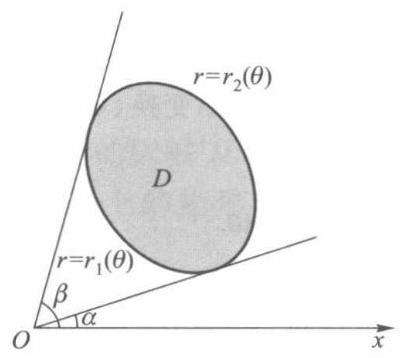
\includegraphics[width=.3\textwidth]{images/P180.jpg}
	\caption{图 $21-25$}
	\label{fig:P180}
\end{figure}

\begin{figure}
	\centering
	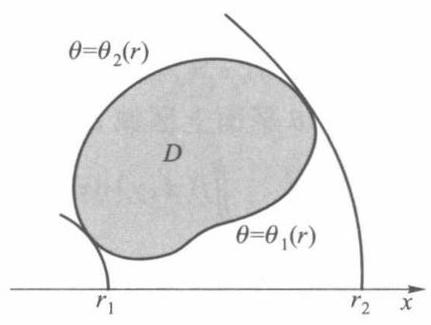
\includegraphics[width=.3\textwidth]{images/P181.jpg}
	\caption{图 $21-26$}
	\label{fig:P181}
\end{figure}

(ii) 若原点为 \(D\) 的内点 (图 21-27), \(D\) 的边界的极坐标方程为 \(r = r\left( \theta \right)\) ,则 \(\Delta\) 可表示成
\[
0 \leq  r \leq  r\left( \theta \right) ,\;0 \leq  \theta  \leq  {2\pi }.
\]
所以
\[
{\iint }_{D}f\left( {x,y}\right) \mathrm{d}x\mathrm{\;d}y = {\int }_{0}^{2\pi }\mathrm{d}\theta {\int }_{0}^{r\left( \theta \right) }f\left( {r\cos \theta ,r\sin \theta }\right) r\mathrm{\;d}r. \tag{12}
\]
(iii) 若原点 \(O\) 在 \(D\) 的边界上 (图21-28),则 \(\Delta\) 为
\[
0 \leq  r \leq  r\left( \theta \right) ,\;\alpha  \leq  \theta  \leq  \beta ,
\]
于是
\[
{\iint }_{D}f\left( {x,y}\right) \mathrm{d}x\mathrm{\;d}y = {\int }_{\alpha }^{\beta }\mathrm{d}\theta {\int }_{0}^{r\left( \theta \right) }f\left( {r\cos \theta ,r\sin \theta }\right) r\mathrm{\;d}r. \tag{13}
\]
\begin{figure}
	\centering
	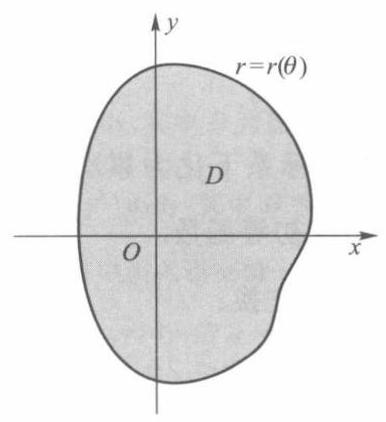
\includegraphics[width=.3\textwidth]{images/P182.jpg}
	\caption{图 $21-27$}
	\label{fig:P182}
\end{figure}

\begin{figure}
	\centering
	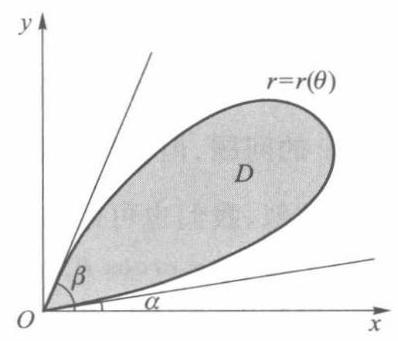
\includegraphics[width=.3\textwidth]{images/P183.jpg}
	\caption{图 $21-28$}
	\label{fig:P183}
\end{figure}

%例 3
\begin{example}

\end{example}
计算
\[
I = {\iint }_{D}\frac{\mathrm{d}\sigma }{\sqrt{1 - {x}^{2} - {y}^{2}}},
\]
其中 \(D\) 为圆域 \({x}^{2} + {y}^{2} \leq  1\) .

%解
\begin{solution}

\end{solution}
由于原点为 \(D\) 的内点,故由 (12) 式,有
\[
{\iint }_{D}\frac{\mathrm{d}\sigma }{\sqrt{1 - {x}^{2} - {y}^{2}}} = {\int }_{0}^{2\pi }\mathrm{d}\theta {\int }_{0}^{1}\frac{r}{\sqrt{1 - {r}^{2}}}\mathrm{\;d}r
\]
\[
= {\int }_{0}^{2\pi }\left\lbrack  {-\sqrt{1 - {r}^{2}}}\right\rbrack  {\left. \right| }_{0}^{1}\mathrm{\;d}\theta  = {\int }_{0}^{2\pi }\mathrm{d}\theta  = {2\pi }.
\]
%例 4
\begin{example}

\end{example}
求球体 \({x}^{2} + {y}^{2} + {z}^{2} \leq  {R}^{2}\) 被圆柱面 \({x}^{2} + {y}^{2} = {Rx}\) 所割下部分的体积 (称为维维安尼 (Viviani) 体).

\begin{figure}
	\centering
	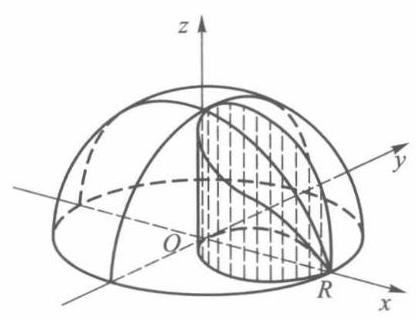
\includegraphics[width=.3\textwidth]{images/P184.jpg}
	\caption{图 $21-29$}
	\label{fig:P184}
\end{figure}

%解
\begin{solution}

\end{solution}
由所求立体的对称性 (图 21-29), 我们只要求出在第一卦限内的部分体积后乘以 4 , 即得所求立体的体积. 在第一卦限内的立体是一个曲顶柱体,其底为 \({xy}\) 平面内由 \(y \geq  0\) 和 \({x}^{2} + {y}^{2} \leq  {Rx}\) 所确定的区域,曲顶的方程为

所以
\[
z = \sqrt{{R}^{2} - {x}^{2} - {y}^{2}}.
\]
\[
V = 4{\iint }_{D}\sqrt{{R}^{2} - {x}^{2} - {y}^{2}}\mathrm{\;d}\sigma ,
\]
其中 \(D = \left\{  {\left( {x,y}\right)  \mid  y \geq  0,{x}^{2} + {y}^{2} \leq  {Rx}}\right\}\) (图21-30). 用极坐标变换后,由 (13) 式,有
\[
V = 4{\int }_{0}^{\frac{\pi }{2}}\mathrm{\;d}\theta {\int }_{0}^{R\cos \theta }\sqrt{{R}^{2} - {r}^{2}}r\mathrm{\;d}r
\]
\[
= \frac{4}{3}{R}^{3}{\int }_{0}^{\frac{\pi }{2}}\left( {1 - {\sin }^{3}\theta }\right) \mathrm{d}\theta  = \frac{4}{3}{R}^{3}\left( {\frac{\pi }{2} - \frac{2}{3}}\right) .
\]
\begin{figure}
	\centering
	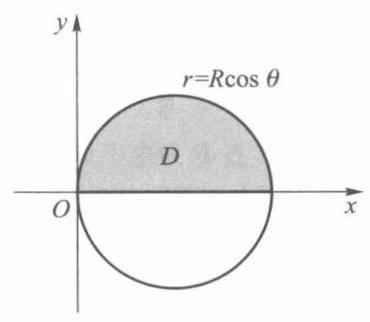
\includegraphics[width=.3\textwidth]{images/P185.jpg}
	\caption{图 $21-30$}
	\label{fig:P185}
\end{figure}

%例 5
\begin{example}

\end{example}
计算 \(I = {\iint }_{D}{\mathrm{e}}^{-\left( {{x}^{2} + {y}^{2}}\right) }\mathrm{d}\sigma\) ,其中 \(D\) 为圆域 \({x}^{2} + {y}^{2} \leq  {R}^{2}\) .

%解
\begin{solution}

\end{solution}
利用极坐标变换, 由公式 (12), 有
\[
I = {\int }_{0}^{2\pi }\mathrm{d}\theta {\int }_{0}^{R}r{\mathrm{e}}^{-{r}^{2}}\mathrm{\;d}r = \pi \left( {1 - {\mathrm{e}}^{-{R}^{2}}}\right) .
\]
由例 5 可见, 若不用极坐标变换计算, 而用直角坐标系下化为累次积分计算, 就会遇到计算 \(\int {\mathrm{e}}^{-{y}^{2}}\mathrm{\;d}y\) 的问题,但我们不能把 \(\int {\mathrm{e}}^{-{y}^{2}}\mathrm{\;d}y\) 表示成初等函数.

与极坐标相类似, 我们也可以作下面的广义极坐标变换:
\[
T : \left\{  {\begin{array}{l} x = \operatorname{arcos}\theta , \\  y = \operatorname{br}\sin \theta , \end{array}\;0 \leq  r <  + \infty ,\;0 \leq  \theta  \leq  {2\pi },}\right.
\]
并计算得
\[
J\left( {r,\theta }\right)  = \left| \begin{array}{rr} a\cos \theta &  - {ar}\sin \theta \\  b\sin \theta & {br}\cos \theta  \end{array}\right|  = {abr}.
\]
对广义极坐标变换也有与定理 21.14 相应的定理, 这里不再赘述了.

%例 6
\begin{example}

\end{example}
求椭球体
\[
\frac{{x}^{2}}{{a}^{2}} + \frac{{y}^{2}}{{b}^{2}} + \frac{{z}^{2}}{{c}^{2}} \leq  1
\]
的体积.

%解
\begin{solution}

\end{solution}
由对称性,椭球体的体积 \(V\) 是第一卦限部分体积的 8 倍,这一部分是以 \(z =\)  \(c\sqrt{1 - \frac{{x}^{2}}{{a}^{2}} - \frac{{y}^{2}}{{b}^{2}}}\) 为曲顶, \(D = \left\{  {\left( {x,y}\right) \left| {\;0 \leq  y \leq  b\sqrt{1 - \frac{{x}^{2}}{{a}^{2}}}}\right. ,0 \leq  x \leq  a}\right\}\) 为底的曲顶柱体,所以
\[
V = 8{\iint }_{D}c\sqrt{1 - \frac{{x}^{2}}{{a}^{2}} - \frac{{y}^{2}}{{b}^{2}}}\mathrm{\;d}x\mathrm{\;d}y.
\]
应用广义极坐标变换,由于 \(z = c\sqrt{1 - {r}^{2}}\) ,因此
\[
V = 8{\int }_{0}^{\frac{\pi }{2}}\mathrm{\;d}\theta {\int }_{0}^{1}c\sqrt{1 - {r}^{2}}{abr}\mathrm{\;d}r
\]
\[
= {8abc}{\int }_{0}^{\frac{\pi }{2}}\mathrm{\;d}\theta {\int }_{0}^{1}r\sqrt{1 - {r}^{2}}\mathrm{\;d}r = \frac{4\pi }{3}{abc}.
\]
当 \(a = b = c = R\) 时,得到球的体积为 \(\frac{4\pi }{3}{R}^{3}\) .

\subsection{习题 21.4}

1. 对积分 \({\iint }_{D}f\left( {x,y}\right) \mathrm{d}x\mathrm{\;d}y\) 进行极坐标变换并写出变换后不同顺序的累次积分:

(1) 当 \(D\) 为由不等式 \({a}^{2} \leq  {x}^{2} + {y}^{2} \leq  {b}^{2},y \geq  0\) 所确定的区域；

(2) \(D = \left\{  {\left( {x,y}\right)  \mid  {x}^{2} + {y}^{2} \leq  y,x \geq  0}\right\}\) ;

(3) \(D = \{ \left( {x,y}\right)  \mid  0 \leq  x \leq  1,0 \leq  x + y \leq  1\}\) .

2. 用极坐标计算下列二重积分:

(1) \({\iint }_{D}\sin \sqrt{{x}^{2} + {y}^{2}}\mathrm{\;d}x\mathrm{\;d}y\) ,其中 \(D = \left\{  {\left( {x,y}\right)  \mid  {\pi }^{2} \leq  {x}^{2} + {y}^{2} \leq  4{\pi }^{2}}\right\}\) ；

( 2 ) \({\iint }_{D}\left( {x + y}\right) \mathrm{d}x\mathrm{\;d}y\) ,其中 \(D = \left\{  {\left( {x,y}\right)  \mid  {x}^{2} + {y}^{2} \leq  x + y}\right\}\) ；

(3) \({\iint }_{D}\left| {xy}\right| \mathrm{d}x\mathrm{\;d}y\) ,其中 \(D\) 为圆域 \({x}^{2} + {y}^{2} \leq  {a}^{2}\) ；

(4) \({\iint }_{D}{f}^{\prime }\left( {{x}^{2} + {y}^{2}}\right) \mathrm{d}x\mathrm{\;d}y\) ,其中 \(D\) 为圆域 \({x}^{2} + {y}^{2} \leq  {R}^{2}\) .

3. 在下列积分中引入新变量 \(u,v\) 后,试将它化为累次积分:

(1) \({\int }_{0}^{2}\mathrm{\;d}x{\int }_{1 - x}^{2 - x}f\left( {x,y}\right) \mathrm{d}y\) ,若 \(u = x + y,v = x - y\) ;

(2) \({\iint }_{D}f\left( {x,y}\right) \mathrm{d}x\mathrm{\;d}y\) ,其中 \(D = \left\{  {\left( {x,y}\right)  \mid  \sqrt{x} + \sqrt{y} \leq  \sqrt{a},x \geq  0,y \geq  0}\right\}\) ,若 \(x = u{\cos }^{4}v,y = u{\sin }^{4}v\) ;

(3) \({\iint }_{D}f\left( {x,y}\right) \mathrm{d}x\mathrm{\;d}y\) ,其中 \(D = \{ \left( {x,y}\right)  \mid  x + y \leq  a,x \geq  0,y \geq  0\}\) ,若 \(x + y = u,y = {uv}\) .

4. 试作适当变换, 计算下列积分:

(1) \({\iint }_{D}\left( {x + y}\right) \sin \left( {x - y}\right) \mathrm{d}x\mathrm{\;d}y,D = \{ \left( {x,y}\right)  \mid  0 \leq  x + y \leq  \pi ,0 \leq  x - y \leq  \pi \}\) ；

(2) \({\iint }_{D}{\mathrm{e}}^{\frac{y}{x + y}}\mathrm{\;d}x\mathrm{\;d}y,D = \{ \left( {x,y}\right)  \mid  x + y \leq  1,x \geq  0,y \geq  0\}\) .

5. 求由下列曲面所围立体 \(V\) 的体积:

(1) \(V\) 是由 \(z = {x}^{2} + {y}^{2}\) 和 \(z = x + y\) 所围的立体；

( 2 ) \(V\) 是由曲面 \({z}^{2} = \frac{{x}^{2}}{4} + \frac{{y}^{2}}{9}\) 和 \({2z} = \frac{{x}^{2}}{4} + \frac{{y}^{2}}{9}\) 所围的立体.

6. 求由下列曲线所围的平面图形面积:

(1) \(x + y = a,x + y = b,y = {\alpha x},y = {\beta x}\left( {0 < a < b,0 < \alpha  < \beta }\right)\) ;

(2) \({\left( \frac{{x}^{2}}{{a}^{2}} + \frac{{y}^{2}}{{b}^{2}}\right) }^{2} = {x}^{2} + {y}^{2}\) ;

(3) \({\left( {x}^{2} + {y}^{2}\right) }^{2} = 2{a}^{2}\left( {{x}^{2} - {y}^{2}}\right) \;\left( {{x}^{2} + {y}^{2} \geq  {a}^{2}}\right)\) .

7. 设 \(f\left( {x,y}\right)\) 为连续函数,且 \(f\left( {x,y}\right)  = f\left( {y,x}\right)\) . 证明
\[
{\int }_{0}^{1}\mathrm{\;d}x{\int }_{0}^{x}f\left( {x,y}\right) \mathrm{d}y = {\int }_{0}^{1}\mathrm{\;d}x{\int }_{0}^{x}f\left( {1 - x,1 - y}\right) \mathrm{d}y.
\]
8. 试作适当变换, 把下列二重积分化为单重积分:

(1) \({\iint }_{D}f\left( \sqrt{{x}^{2} + {y}^{2}}\right) \mathrm{d}x\mathrm{\;d}y\) ,其中 \(D\) 为圆域 \({x}^{2} + {y}^{2} \leq  1\) ；

(2) \({\iint }_{D}f\left( \sqrt{{x}^{2} + {y}^{2}}\right) \mathrm{d}x\mathrm{\;d}y\) ,其中 \(D = \{ \left( {x,y}\right) \left| \right| y\left|  \leq  \right| x\left| ,\right| x \mid   \leq  1\}\) ；

(3) \({\iint }_{D}f\left( {x + y}\right) \mathrm{d}x\mathrm{\;d}y\) ,其中 \(D = \{ \left( {x,y}\right) \left| \right| x\left| +\right| y \mid   \leq  1\}\) ；

(4) \({\iint }_{D}f\left( {xy}\right) \mathrm{d}x\mathrm{\;d}y\) ,其中 \(D = \{ \left( {x,y}\right)  \mid  x \leq  y \leq  {4x},1 \leq  {xy} \leq  2\}\) .

\section{三重积分}

\subsection{三重积分的概念}

类似于第一型曲线积分,求一个空间立体 \(V\) 的质量 \(M\) 就可导出三重积分. 设密度函数为 \(f\left( {x,y,z}\right)\) ,为了求 \(V\) 的质量,我们把 \(V\) 分割成 \(n\) 个小块 \({V}_{1},{V}_{2},\cdots ,{V}_{n}\) ,在每个小块 \({V}_{i}\) 上任取一点 \(\left( {{\xi }_{i},{\eta }_{i},{\zeta }_{i}}\right)\) ,则
\[
M = \mathop{\lim }\limits_{{\parallel T\parallel  \rightarrow  0}}\mathop{\sum }\limits_{{i = 1}}^{n}f\left( {{\xi }_{i},{\eta }_{i},{\zeta }_{i}}\right) \Delta {V}_{i},
\]
其中 \(\Delta {V}_{i}\) 为小块 \({V}_{i}\) 的体积, \(\parallel T\parallel  = \mathop{\max }\limits_{{1 \leq  i \leq  n}}\left\{  {V}_{i}\right\}\) 的直径 \(\}\) .

设 \(f\left( {x,y,z}\right)\) 是定义在三维空间可求体积的有界闭区域 \({V}\)\footnote{读者可仿照 §1 定义平面图形可求面积的方法建立空间立体可求体积的概念. 今后我们总假定 \(V\) 的边界由光滑曲面组成, 以保证积分区域是可求体积的.} 上的有界函数. 现用若干光滑曲面所组成的曲面网 \(T\) 来分割 \(V\) ,它把 \(V\) 分成 \(n\) 个小区域 \({V}_{1},{V}_{2},\cdots ,{V}_{n}\) . 记 \({V}_{i}\) 的体积为 \(\Delta {V}_{i}\left( {i = 1,2,\cdots ,n}\right) ,\parallel T\parallel  = \mathop{\max }\limits_{{1 \leq  i \leq  n}}\left\{  {V}_{i}\right\}\) 的直径 \(\}\) . 在每个 \({V}_{i}\) 中任取一点 \(\left( {{\xi }_{i},{\eta }_{i},{\zeta }_{i}}\right)\) , 作积分和
\[
\mathop{\sum }\limits_{{i = 1}}^{n}f\left( {{\xi }_{i},{\eta }_{i},{\zeta }_{i}}\right) \Delta {V}_{i}.
\]
%定义  1
\begin{definition}{}{def:}

\end{definition}
设 \(f\left( {x,y,z}\right)\) 为定义在三维空间可求体积的有界闭区域 \(V\) 上的函数, \(J\) 是一个确定的数. 若对任给的正数 \(\varepsilon\) ,总存在某一正数 \(\delta\) ,使得对于 \(V\) 的任何分割 \(T\) ,只要 \(\parallel T\parallel  < \delta\) ,属于分割 \(T\) 的所有积分和都有
\[
\left| {\mathop{\sum }\limits_{{i = 1}}^{n}f\left( {{\xi }_{i},{\eta }_{i},{\zeta }_{i}}\right) \Delta {V}_{i} - J}\right|  < \varepsilon ,
\]
则称 \(f\left( {x,y,z}\right)\) 在 \(V\) 上可积,数 \(J\) 称为函数 \(f\left( {x,y,z}\right)\) 在 \(V\) 上的三重积分,记作
\[
J = {\iiint }_{V}f\left( {x,y,z}\right) \mathrm{d}V\text{ 或 }J = {\iiint }_{V}f\left( {x,y,z}\right) \mathrm{d}x\mathrm{\;d}y\mathrm{\;d}z,
\]
其中 \(f\left( {x,y,z}\right)\) 称为被积函数, \(x,y,z\) 称为积分变量, \(V\) 称为积分区域.

当 \(f\left( {x,y,z}\right)  \equiv  1\) 时, \({\iiint }_{V}\mathrm{\;d}V\) 在几何上表示 \(V\) 的体积.

三重积分具有与二重积分相应的可积条件和有关性质 (参见 §1 ),这里不一一细述了. 例如, 类似于二重积分, 有

(i) 有界闭区域 \(V\) 上的连续函数必可积;

(ii) 如果有界闭区域 \(V\) 上的有界函数 \(f\left( {x,y,z}\right)\) 的间断点集中在有限多个零体积 (可类似于零面积那样来定义) 的曲面上,则 \(f\left( {x,y,z}\right)\) 在 \(V\) 上必可积.

\subsection{化三重积分为累次积分}

%定理 21.15
\begin{theorem}{}{the:}

\end{theorem}
 若函数 \(f\left( {x,y,z}\right)\) 在长方体 \(V = \left\lbrack  {a,b}\right\rbrack   \times  \left\lbrack  {c,d}\right\rbrack   \times  \left\lbrack  {e,h}\right\rbrack\) 上的三重积分存在,且对任意 \(\left( {x,y}\right)  \in  D = \left\lbrack  {a,b}\right\rbrack   \times  \left\lbrack  {c,d}\right\rbrack  ,g\left( {x,y}\right)  = {\int }_{e}^{h}f\left( {x,y,z}\right) \mathrm{d}z\) 存在,则积分 \({\iint }_{D}g\left( {x,y}\right) \mathrm{d}x\mathrm{\;d}y\) 也存在, 且
\[
{\iiint }_{V}f\left( {x,y,z}\right) \mathrm{d}x\mathrm{\;d}y\mathrm{\;d}z = {\iint }_{D}\mathrm{\;d}x\mathrm{\;d}y{\int }_{e}^{h}f\left( {x,y,z}\right) \mathrm{d}z. \tag{1}
\]
%证
\begin{proof}

\end{proof}
用平行于坐标平面的平面作分割 \(T\) ,它把 \(V\) 分成有限多个小长方体
\[
{V}_{ijk} = \left\lbrack  {{x}_{i - 1},{x}_{i}}\right\rbrack   \times  \left\lbrack  {{y}_{j - 1},{y}_{j}}\right\rbrack   \times  \left\lbrack  {{z}_{k - 1},{z}_{k}}\right\rbrack  .
\]
设 \({M}_{ijk},{m}_{ijk}\) 分别是 \(f\left( {x,y,z}\right)\) 在 \({V}_{ijk}\) 上的上确界和下确界. 对任意
\[
\left( {{\xi }_{i},{\eta }_{j}}\right)  \in  \left\lbrack  {{x}_{i - 1},{x}_{i}}\right\rbrack   \times  \left\lbrack  {{y}_{j - 1},{y}_{j}}\right\rbrack  ,
\]
\[
{m}_{ijk}\Delta {z}_{k} \leq  {\int }_{{z}_{k - 1}}^{{z}_{k}}f\left( {{\xi }_{i},{\eta }_{j},z}\right) \mathrm{d}z \leq  {M}_{ijk}\Delta {z}_{k}.
\]
现按下标 \(k\) 相加,有
\[
\mathop{\sum }\limits_{k}{\int }_{{z}_{k - 1}}^{{z}_{k}}f\left( {{\xi }_{i},{\eta }_{j},z}\right) \mathrm{d}z = {\int }_{e}^{h}f\left( {{\xi }_{i},{\eta }_{j},z}\right) \mathrm{d}z = g\left( {{\xi }_{i},{\eta }_{j}}\right)
\]
以及
\[
\mathop{\sum }\limits_{{i,j,k}}{m}_{ijk}\Delta {x}_{i}\Delta {y}_{j}\Delta {z}_{k} \leq  \mathop{\sum }\limits_{{i,j}}g\left( {{\xi }_{i},{\eta }_{j}}\right) \Delta {x}_{i}\Delta {y}_{j} \leq  \mathop{\sum }\limits_{{i,j,k}}{M}_{ijk}\Delta {x}_{i}\Delta {y}_{j}\Delta {z}_{k}. \tag{2}
\]
上述不等式两边是分割 \(T\) 的下和与上和. 由 \(f\left( {x,y,z}\right)\) 在 \(V\) 上可积,当 \(\parallel T\parallel  \rightarrow  0\) 时,下和与上和具有相同的极限,所以由 (2) 式得 \(g\left( {x,y}\right)\) 关于 \(D\) 对应 \(T\) 的直线网格分割的下和与上和具有相同的极限. 由定理 21.4 有 \(g\left( {x,y}\right)\) 在 \(D\) 上可积,且
\[
{\iint }_{D}g\left( {x,y}\right) \mathrm{d}x\mathrm{\;d}y = {\iiint }_{V}f\left( {x,y,z}\right) \mathrm{d}x\mathrm{\;d}y\mathrm{\;d}z.
\]
推论 若 \(V = \left\{  {\left( {x,y,z}\right)  \mid  \left( {x,y}\right)  \in  D,{z}_{1}\left( {x,y}\right)  \leq  z \leq  {z}_{2}\left( {x,y}\right) }\right\}   \subset  \left\lbrack  {a,b}\right\rbrack   \times  \left\lbrack  {c,d}\right\rbrack   \times  \lbrack e\) , \(h\rbrack\) ,其中 \(D\) 为 \(V\) 在 \({Oxy}\) 平面上的投影, \({z}_{1}\left( {x,y}\right) ,{z}_{2}\left( {x,y}\right)\) 是 \(D\) 上的连续函数,函数 \(f\left( {x,y,z}\right)\) 在 \(V\) 上的三重积分存在,且对任意 \(\left( {x,y}\right)  \in  D\) ,
\[
G\left( {x,y}\right)  = {\int }_{{z}_{1}\left( {x,y}\right) }^{{z}_{2}\left( {x,y}\right) }f\left( {x,y,z}\right) \mathrm{d}z
\]
亦存在,则积分 \({\iint }_{D}G\left( {x,y}\right) \mathrm{d}x\mathrm{\;d}y\) 存在,且
\[
{\iint }_{V}f\left( {x,y,z}\right) \mathrm{d}x\mathrm{\;d}y\mathrm{\;d}z = {\iint }_{D}G\left( {x,y}\right) \mathrm{d}x\mathrm{\;d}y = {\iint }_{D}\mathrm{\;d}x\mathrm{\;d}y{\int }_{{z}_{1}\left( {x,y}\right) }^{{z}_{2}\left( {x,y}\right) }f\left( {x,y,z}\right) \mathrm{d}z. \tag{3}
\]
(见图 21-31).

%证
\begin{proof}

\end{proof}
定义 \(F\left( {x,y,z}\right)  = \left\{  \begin{array}{ll} f\left( {x,y,z}\right) , & \left( {x,y,z}\right)  \in  V, \\  0, & \left( {x,y,z}\right)  \in  {V}_{0} \smallsetminus  V, \end{array}\right.\) 其中 \({V}_{0} = \left\lbrack  {a,b}\right\rbrack   \times  \left\lbrack  {c,d}\right\rbrack   \times  \left\lbrack  {e\text{ , }}\right\rbrack\)  \(h\rbrack\) ,对 \(F\left( {x,y,z}\right)\) 用定理 21.15,则有
\[
{\iiint }_{V}f\left( {x,y,z}\right) \mathrm{d}x\mathrm{\;d}y\mathrm{\;d}z = {\iiint }_{{V}_{0}}F\left( {x,y,z}\right) \mathrm{d}x\mathrm{\;d}y\mathrm{\;d}z
\]
\[
= {\iint }_{\left\lbrack  {a,b}\right\rbrack   \times  \left\lbrack  {c,d}\right\rbrack  }\mathrm{d}x\mathrm{\;d}y{\int }_{e}^{h}F\left( {x,y,z}\right) \mathrm{d}z
\]
\[
= {\iint }_{D}\mathrm{\;d}x\mathrm{\;d}y{\int }_{{z}_{1}\left( {x,y}\right) }^{{z}_{2}\left( {x,y}\right) }f\left( {x,y,z}\right) \mathrm{d}z.
\]
\begin{figure}
	\centering
	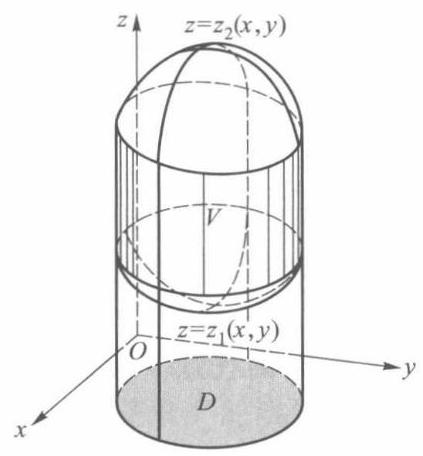
\includegraphics[width=.3\textwidth]{images/P186.jpg}
	\caption{图 $21-31$}
	\label{fig:P186}
\end{figure}

\begin{figure}
	\centering
	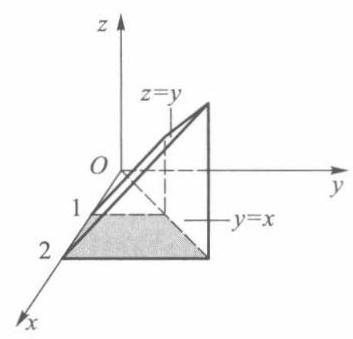
\includegraphics[width=.3\textwidth]{images/P187.jpg}
	\caption{图 $21-32$}
	\label{fig:P187}
\end{figure}

%例 1
\begin{example}

\end{example}
计算 \({\iiint }_{V}\frac{\mathrm{d}x\mathrm{\;d}y\mathrm{\;d}z}{{x}^{2} + {y}^{2}}\) ,其中 \(V\) 为由平面 \(x = 1,x = 2,z = 0,y = x\) 与 \(z = y\) 所围区域 (见图 21-32)

%解
\begin{solution}

\end{solution}
设 \(V\) 在 \({xy}\) 平面上投影为 \(D\) ,则 \(V = \left\{  {\left( {x,y,z}\right)  \mid  {z}_{1}\left( {x,y}\right)  \leq  z \leq  {z}_{2}\left( {x,y}\right) }\right.\) , \(\left( {x,y}\right)  \in  D\}\) ,其中 \(D = \{ \left( {x,y}\right)  \mid  0 \leq  y \leq  x,1 \leq  x \leq  2\}\) 是 \(x\) 型区域, \({z}_{1}\left( {x,y}\right)  = 0,{z}_{2}\left( {x,y}\right)  = y\) . 于是
\[
{\iiint }_{V}\frac{\mathrm{d}x\mathrm{\;d}y\mathrm{\;d}z}{{x}^{2} + {y}^{2}} = {\iint }_{D}\mathrm{\;d}x\mathrm{\;d}y{\int }_{0}^{y}\frac{\mathrm{d}z}{{x}^{2} + {y}^{2}}
\]
\[
= {\iint }_{D}\frac{y}{{x}^{2} + {y}^{2}}\mathrm{\;d}x\mathrm{\;d}y = {\int }_{1}^{2}\mathrm{\;d}x{\int }_{0}^{x}\frac{y\mathrm{\;d}y}{{x}^{2} + {y}^{2}}
\]
\[
= {\int }_{1}^{2}{\left. \frac{1}{2}\ln \left( {x}^{2} + {y}^{2}\right) \right| }_{0}^{x}\mathrm{\;d}x = {\int }_{1}^{2}\frac{1}{2}\ln 2\mathrm{\;d}x
\]
\[
= \frac{1}{2}\ln 2\text{ . }
\]
%例 2
\begin{example}

\end{example}
计算 \({\iint }_{V}\left( {{x}^{2} + {y}^{2} + z}\right) \mathrm{d}x\mathrm{\;d}y\mathrm{\;d}z\) ,其中 \(V\) 是由 \(\left\{  \begin{array}{l} z = y, \\  x = 0 \end{array}\right.\) 绕 \(z\) 轴旋转一周而成的曲面与 \(z = 1\) 所围的区域.

%解
\begin{solution}

\end{solution}
旋转面方程为 \(z = \sqrt{{x}^{2} + {y}^{2}},V\) 在 \({xy}\) 平面上投影为 \(D = \left\{  {\left( {x,y}\right)  \mid  {x}^{2} + {y}^{2} \leq  1}\right\}\) , \({z}_{1}\left( {x,y}\right)  = \sqrt{{x}^{2} + {y}^{2}},{z}_{2}\left( {x,y}\right)  = 1\) ,于是
\[
{\iiint }_{V}\left( {{x}^{2} + {y}^{2} + z}\right) \mathrm{d}x\mathrm{\;d}y\mathrm{\;d}z = {\iint }_{D}\mathrm{\;d}x\mathrm{\;d}y{\int }_{\sqrt{{x}^{2} + {y}^{2}}}^{1}\left( {{x}^{2} + {y}^{2} + z}\right) \mathrm{d}z
\]
\[
= {\iint }_{D}\left( {{x}^{2} + {y}^{2}}\right) \left( {1 - \sqrt{{x}^{2} + {y}^{2}}}\right) \mathrm{d}x\mathrm{\;d}y + \frac{1}{2}{\iint }_{D}\left\lbrack  {1 - \left( {{x}^{2} + {y}^{2}}\right) }\right\rbrack  \mathrm{d}x\mathrm{\;d}y
\]
\[
= {\int }_{0}^{2\pi }\mathrm{d}\theta {\int }_{0}^{1}{r}^{2}\left( {1 - r}\right) r\mathrm{\;d}r + \frac{1}{2}{\int }_{0}^{2\pi }\mathrm{d}\theta {\int }_{0}^{1}\left( {1 - {r}^{2}}\right) r\mathrm{\;d}r
\]
\[
= \frac{\pi }{10} + \frac{\pi }{4} = \frac{7\pi }{20}\text{ . }
\]
类似分析可得到以下定理和推论.

%定理 21.16
\begin{theorem}{}{the:}

\end{theorem}
 若函数 \(f\left( {x,y,z}\right)\) 在长方体 \(V = \left\lbrack  {a,b}\right\rbrack   \times  \left\lbrack  {c,d}\right\rbrack   \times  \left\lbrack  {e,h}\right\rbrack\) 上的三重积分存在,且对任何 \(z \in  \left\lbrack  {e,h}\right\rbrack\) ,二重积分
\[
I\left( z\right)  = {\iint }_{D}f\left( {x,y,z}\right) \mathrm{d}x\mathrm{\;d}y
\]
存在,其中 \(D = \left\lbrack  {a,b}\right\rbrack   \times  \left\lbrack  {c,d}\right\rbrack\) ,则积分
\[
{\int }_{e}^{h}\mathrm{\;d}z{\iint }_{D}f\left( {x,y,z}\right) \mathrm{d}x\mathrm{\;d}y
\]
也存在,且
\[
{\iiint }_{V}f\left( {x,y,z}\right) \mathrm{d}x\mathrm{\;d}y\mathrm{\;d}z = {\int }_{e}^{h}\mathrm{\;d}z{\iint }_{D}f\left( {x,y,z}\right) \mathrm{d}x\mathrm{\;d}y.
\]
推论 若 \(V \subset  \left\lbrack  {a,b}\right\rbrack   \times  \left\lbrack  {c,d}\right\rbrack   \times  \left\lbrack  {e,h}\right\rbrack\) ,函数 \(f\left( {x,y,z}\right)\) 在 \(V\) 上的三重积分存在,且对任意固定的 \(z \in  \left\lbrack  {e,h}\right\rbrack\) ,积分 \(\varphi \left( z\right)  = {\iint }_{{D}_{z}}f\left( {x,y,z}\right) \mathrm{d}x\mathrm{\;d}y\) 存在,其中 \({D}_{z}\) 是截面 \(\{ \left( {x,y}\right)  \mid  \left( {x,y,z}\right)  \in  V\}\) ,则 \({\int }_{e}^{h}\varphi \left( z\right) \mathrm{d}z\) 存在,且
\[
{\iiint }_{V}f\left( {x,y,z}\right) \mathrm{d}x\mathrm{\;d}y\mathrm{\;d}z = {\int }_{e}^{h}\varphi \left( z\right) \mathrm{d}z = {\int }_{e}^{h}\mathrm{\;d}z{\iint }_{{D}_{z}}f\left( {x,y,z}\right) \mathrm{d}x\mathrm{\;d}y.
\]
(见图 21-33).

%注
\begin{remark}

\end{remark}
类似于对二重积分转化为累次积分的几何解释, 对定理 21.15 和定理 21.16 及其推论所给出的方法也可以从几何上做出解释. 在定理 21.15 及其推论中, 把积分区域视为柱体的一部分 (见图 21-31),投影 (柱体底面) 区域为 \(D\) ,柱体上、下曲面分别为 \(z = {z}_{2}\left( {x,y}\right) ,z = {z}_{1}\left( {x,y}\right) ,\left( {x,y}\right)  \in  D\) . 三重积分相应转化为先对 \(z\) 再对 \(x,y\) 的累次积分形式 (先一后二). 在定理 21.16 及其推论中,把积分区域视为介于两平行平面 \(z = e\) , \(z = h\) 之间的立体 (见图 21-33),用垂直于 \(z\) 轴的面截积分区域所得截面为 \({D}_{z}\) . 此时三重积分相应转化为先对 \(x,y\) 变量在平面区域 \({D}_{z}\) 上的含参二重积分,再对 \(z \in  \left\lbrack  {e,h}\right\rbrack\) 求定积分的形式 (先二后一). 具体采用哪一种形式可根据实际问题中积分区域与被积函数的特性加以选择.

\begin{figure}
	\centering
	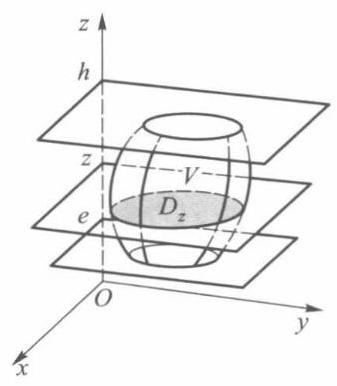
\includegraphics[width=.3\textwidth]{images/P188.jpg}
	\caption{图 $21-33$}
	\label{fig:P188}
\end{figure}

%例 3
\begin{example}

\end{example}
求
\[
I = {\iiint }_{V}\left( {\frac{{x}^{2}}{{a}^{2}} + \frac{{y}^{2}}{{b}^{2}} + \frac{{z}^{2}}{{c}^{2}}}\right) \mathrm{d}x\mathrm{\;d}y\mathrm{\;d}z,
\]
其中 \(V\) 是椭球体 \(\frac{{x}^{2}}{{a}^{2}} + \frac{{y}^{2}}{{b}^{2}} + \frac{{z}^{2}}{{c}^{2}} \leq  1\) .

%解
\begin{solution}

\end{solution}
由于
\[
I = {\iiint }_{V}\frac{{x}^{2}}{{a}^{2}}\mathrm{\;d}x\mathrm{\;d}y\mathrm{\;d}z + {\iiint }_{V}\frac{{y}^{2}}{{b}^{2}}\mathrm{\;d}x\mathrm{\;d}y\mathrm{\;d}z + {\iiint }_{V}\frac{{z}^{2}}{{c}^{2}}\mathrm{\;d}x\mathrm{\;d}y\mathrm{\;d}z,
\]
其中 \({\iiint }_{V}\frac{{x}^{2}}{{a}^{2}}\mathrm{\;d}x\mathrm{\;d}y\mathrm{\;d}z = {\int }_{-a}^{a}\frac{{x}^{2}}{{a}^{2}}\mathrm{\;d}x{\iint }_{{V}_{x}}\mathrm{\;d}y\mathrm{\;d}z\) ,这里 \({V}_{x}\) 表示椭圆面
\[
\frac{{y}^{2}}{{b}^{2}} + \frac{{z}^{2}}{{c}^{2}} \leq  1 - \frac{{x}^{2}}{{a}^{2}}\text{ 或 }\frac{{y}^{2}}{{b}^{2}\left( {1 - \frac{{x}^{2}}{{a}^{2}}}\right) } + \frac{{z}^{2}}{{c}^{2}\left( {1 - \frac{{x}^{2}}{{a}^{2}}}\right) } \leq  1.
\]
它的面积为
\[
\pi \left( {b\sqrt{1 - \frac{{x}^{2}}{{a}^{2}}}}\right) \left( {c\sqrt{1 - \frac{{x}^{2}}{{a}^{2}}}}\right)  = {\pi bc}\left( {1 - \frac{{x}^{2}}{{a}^{2}}}\right) .
\]
于是
\[
{\iiint }_{V}\frac{{x}^{2}}{{a}^{2}}\mathrm{\;d}x\mathrm{\;d}y\mathrm{\;d}z = {\int }_{-a}^{a}\frac{\pi bc}{{a}^{2}}{x}^{2}\left( {1 - \frac{{x}^{2}}{{a}^{2}}}\right) \mathrm{d}x = \frac{4}{15}{\pi abc}.
\]
同理可得
\[
{\iiint }_{V}\frac{{y}^{2}}{{b}^{2}}\mathrm{\;d}x\mathrm{\;d}y\mathrm{\;d}z = \frac{4}{15}{\pi abc},{\iiint }_{V}\frac{{z}^{2}}{{c}^{2}}\mathrm{\;d}x\mathrm{\;d}y\mathrm{\;d}z = \frac{4}{15}{\pi abc}.
\]
所以
\[
I = 3\left( {\frac{4}{15}{\pi abc}}\right)  = \frac{4}{5}{\pi abc}.
\]
下面用定理 21.16 的推论计算例 1 .

%例 1
\begin{example}

\end{example}
中的区域 \(V = \left\{  {\left( {x,y,z}\right)  \mid  1 \leq  x \leq  2,\left( {y,z}\right)  \in  {D}_{x}}\right\}\) ,其中 \({D}_{x} = \{ \left( {y,z}\right)  \mid  0 \leq  y \leq  x,0 \leq  z \leq  y\}\) (见图 21-34).
\[
{\iiint }_{V}\frac{\mathrm{d}x\mathrm{\;d}y\mathrm{\;d}z}{{x}^{2} + {y}^{2}} = {\int }_{1}^{2}\mathrm{\;d}x{\iint }_{{D}_{x}}\frac{\mathrm{d}y\mathrm{\;d}z}{{x}^{2} + {y}^{2}}
\]
\[
= {\int }_{1}^{2}\mathrm{\;d}x{\int }_{0}^{x}\mathrm{\;d}y{\int }_{0}^{y}\frac{\mathrm{d}z}{{x}^{2} + {y}^{2}}
\]
\[
= {\int }_{1}^{2}\mathrm{\;d}x{\int }_{0}^{x}\frac{y\mathrm{\;d}y}{{x}^{2} + {y}^{2}} = \frac{1}{2}\ln 2.
\]
\begin{figure}
	\centering
	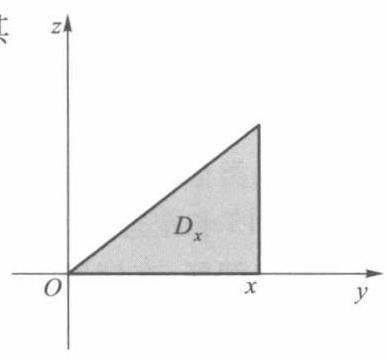
\includegraphics[width=.3\textwidth]{images/P189.jpg}
	\caption{图 $21-34$}
	\label{fig:P189}
\end{figure}

\subsection{三重积分换元法}

和二重积分一样, 某些类型的三重积分作适当的变量变换后能使计算方便.

设变换 \(T : x = x\left( {u,v,w}\right) ,y = y\left( {u,v,w}\right) ,z = z\left( {u,v,w}\right)\) ,把 \({uvw}\) 空间中的区域 \({V}^{\prime }\) 一对一地映成 \({xyz}\) 空间中的区域 \(V\) ,并设函数 \(x\left( {u,v,w}\right) ,y\left( {u,v,w}\right) ,z\left( {u,v,w}\right)\) 及它们的一阶偏导数在 \({V}^{\prime }\) 内连续且函数行列式
\[
J\left( {u,v,w}\right)  = \left| \begin{array}{lll} \frac{\partial x}{\partial u} & \frac{\partial x}{\partial v} & \frac{\partial x}{\partial w} \\  \frac{\partial y}{\partial u} & \frac{\partial y}{\partial v} & \frac{\partial y}{\partial w} \\  \frac{\partial z}{\partial u} & \frac{\partial z}{\partial v} & \frac{\partial z}{\partial w} \end{array}\right|  \neq  0,\left( {u,v,w}\right)  \in  {V}^{\prime }.
\]
于是与二重积分换元法一样,可以证明 (用本章 §9 中证明二重积分类似的方法) 成立下面的三重积分换元公式:
\[
{\iiint }_{V}f\left( {x,y,z}\right) \mathrm{d}x\mathrm{\;d}y\mathrm{\;d}z
\]
\[
= {\iiint }_{{V}^{\prime }}f\left( {x\left( {u,v,w}\right) ,y\left( {u,v,w}\right) ,z\left( {u,v,w}\right) }\right) \left| {J\left( {u,v,w}\right) }\right| \mathrm{d}u\mathrm{\;d}v\mathrm{\;d}w, \tag{4}
\]
其中 \(f\left( {x,y,z}\right)\) 在 \(V\) 上可积.

下面介绍几个常用的变换公式:

1. 柱面坐标变换
\[
T : \left\{  \begin{array}{ll} x = r\cos \theta , & 0 \leq  r <  + \infty , \\  y = r\sin \theta , & 0 \leq  \theta  \leq  {2\pi }, \\  z = z, &  - \infty  < z <  + \infty . \end{array}\right.
\]
由于变换 \(T\) 的函数行列式
\[
J\left( {r,\theta ,z}\right)  = \left| \begin{matrix} \cos \theta &  - r\sin \theta & 0 \\  \sin \theta & r\cos \theta & 0 \\  0 & 0 & 1 \end{matrix}\right|  = r,
\]
按 (4) 式, 三重积分的柱面坐标换元公式为
\[
{\iiint }_{V}f\left( {x,y,z}\right) \mathrm{d}x\mathrm{\;d}y\mathrm{\;d}z = {\iiint }_{{V}^{\prime }}f\left( {r\cos \theta ,r\sin \theta ,z}\right) r\mathrm{\;d}r\mathrm{\;d}\theta \mathrm{d}z, \tag{5}
\]
这里 \({V}^{\prime }\) 为 \(V\) 在柱面坐标变换下的原象.

与极坐标变换一样,柱面坐标变换并非是一对一的,并且当 \(r = 0\) 时, \(J\left( {r,\theta ,z}\right)  = 0\) , 但我们仍可证明 (5) 式成立.

在柱面坐标系中,用 \(r =\) 常数, \(\theta  =\) 常数, \(z =\) 常数的平面分割 \({V}^{\prime }\) 时,变换后在 \({xyz}\) 直角坐标系中, \(r =\) 常数是以 \(z\) 轴为中心轴的圆柱面, \(\theta  =\) 常数是过 \(z\) 轴的半平面, \(z =\) 常数是垂直于 \(z\) 轴的平面 (图 21-35).

用柱面坐标计算三重积分,通常是找出 \(V\) 在 \({xy}\) 平面上的投影区域 \(D\) ,即当
\[
V = \left\{  {\left( {x,y,z}\right)  \mid  {z}_{1}\left( {x,y}\right)  \leq  z \leq  {z}_{2}\left( {x,y}\right) ,\left( {x,y}\right)  \in  D}\right\}
\]
时,
\[
{\iiint }_{V}f\left( {x,y,z}\right) \mathrm{d}x\mathrm{\;d}y\mathrm{\;d}z = {\iint }_{D}\mathrm{\;d}x\mathrm{\;d}y{\int }_{{z}_{1}\left( {x,y}\right) }^{{z}_{2}\left( {x,y}\right) }f\left( {x,y,z}\right) \mathrm{d}z,
\]
其中二重积分部分应用极坐标计算.

%例 4
\begin{example}

\end{example}
计算
\[
{\iiint }_{V}\left( {{x}^{2} + {y}^{2}}\right) \mathrm{d}x\mathrm{\;d}y\mathrm{\;d}z,
\]
其中 \(V\) 是由曲面 \(2\left( {{x}^{2} + {y}^{2}}\right)  = z\) 与 \(z = 4\) 为界面的区域 (图 21-36).

\begin{figure}
	\centering
	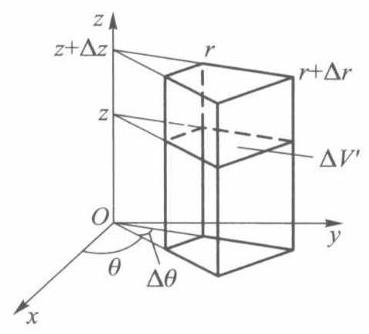
\includegraphics[width=.3\textwidth]{images/P190.jpg}
	\caption{图 $21-35$}
	\label{fig:P190}
\end{figure}

\begin{figure}
	\centering
	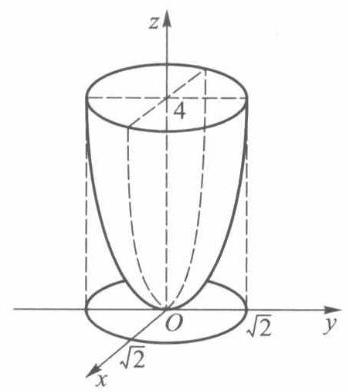
\includegraphics[width=.3\textwidth]{images/P191.jpg}
	\caption{图 $21-36$}
	\label{fig:P191}
\end{figure}

%解
\begin{solution}

\end{solution}
\(V\) 在 \({xy}\) 平面上的投影区域 \(D\) 为 \({x}^{2} + {y}^{2} \leq  2\) . 按柱坐标变换,区域 \({V}^{\prime }\) 可表为
\[
{V}^{\prime } = \left\{  {\left( {r,\theta ,z}\right)  \mid  2{r}^{2} \leq  z \leq  4,0 \leq  r \leq  \sqrt{2},0 \leq  \theta  \leq  {2\pi }}\right\}  .
\]
所以由公式 (5), 有
\[
{\iiint }_{V}\left( {{x}^{2} + {y}^{2}}\right) \mathrm{d}x\mathrm{\;d}y\mathrm{\;d}z = {\iiint }_{{V}^{\prime }}{r}^{3}\mathrm{\;d}r\mathrm{\;d}\theta \mathrm{d}z
\]
\[
= {\int }_{0}^{2\pi }\mathrm{d}\theta {\int }_{0}^{\sqrt{2}}\mathrm{\;d}r{\int }_{2{r}^{2}}^{4}{r}^{3}\mathrm{\;d}z = \frac{8\pi }{3}.
\]
2. 球坐标变换
\[
T : \left\{  \begin{array}{ll} x = r\sin \varphi \cos \theta , & 0 \leq  r <  + \infty , \\  y = r\sin \varphi \sin \theta , & 0 \leq  \varphi  \leq  \pi , \\  z = r\cos \varphi , & 0 \leq  \theta  \leq  {2\pi }. \end{array}\right.
\]
由于
\[
J\left( {r,\varphi ,\theta }\right)  = \left| \begin{matrix} \sin \varphi \cos \theta & r\cos \varphi \cos \theta &  - r\sin \varphi \sin \theta \\  \sin \varphi \sin \theta & r\cos \varphi \sin \theta & r\sin \varphi \cos \theta \\  \cos \varphi &  - r\sin \varphi & 0 \end{matrix}\right|
\]
\[
= {r}^{2}\sin \varphi \text{ , }
\]
当 \(\varphi\) 在 \(\left\lbrack  {0,\pi }\right\rbrack\) 上取值时, \(\sin \varphi  \geq  0\) ,所以在球坐标变换下,按公式 (4),三重积分的球坐标换元公式为
\[
{\iiint }_{V}f\left( {x,y,z}\right) \mathrm{d}x\mathrm{\;d}y\mathrm{\;d}z
\]
\[
= {\iiint }_{{V}^{\prime }}f\left( {r\sin \varphi \cos \theta ,r\sin \varphi \sin \theta ,r\cos \varphi }\right) {r}^{2}\sin \varphi \mathrm{d}r\mathrm{\;d}\varphi \mathrm{d}\theta \text{ , } \tag{6}
\]
这里 \({V}^{\prime }\) 为 \(V\) 在球坐标变换 \(T\) 下的原象.

类似地,球坐标变换并不是一对一的,并且当 \(r = 0\) 或 \(\varphi  = 0\) 或 \(\pi\) 时, \(J\left( {r,\varphi ,\theta }\right)  = 0\) . 但我们仍然可以证明 (6) 式成立.

在球坐标系中,用 \(r =\) 常数, \(\varphi  =\) 常数, \(\theta  =\) 常数的平面分割 \({V}^{\prime }\) 时,变换后在 \({xyz}\) 直角坐标系中, \(r =\) 常数是以原点为心的球面, \(\varphi  =\) 常数是以原点为顶点、 \(z\) 轴为中心轴的半圆锥面, \(\theta  =\) 常数是过 \(z\) 轴的半平面 (图 21-37).

在球坐标系下,当区域 \({V}^{\prime }\) 为集合
\[
{V}^{\prime } = \left\{  {\left( {r,\varphi ,\theta }\right)  \mid  {r}_{1}\left( {\varphi ,\theta }\right)  \leq  r \leq  {r}_{2}\left( {\varphi ,\theta }\right) ,{\varphi }_{1}\left( \theta \right)  \leq  \varphi  \leq  {\varphi }_{2}\left( \theta \right) ,{\theta }_{1} \leq  \theta  \leq  {\theta }_{2}}\right\}
\]
时, (6) 式可化为累次积分
\[
{\iiint }_{V}f\left( {x,y,z}\right) \mathrm{d}x\mathrm{\;d}y\mathrm{\;d}z
\]
\[
= {\int }_{{\theta }_{1}}^{{\theta }_{2}}\mathrm{\;d}\theta {\int }_{{\varphi }_{1}\left( \theta \right) }^{{\varphi }_{2}\left( \theta \right) }\mathrm{d}\varphi {\int }_{{r}_{1}\left( {\varphi ,\theta }\right) }^{{r}_{2}\left( {\varphi ,\theta }\right) }f\left( {r\sin \varphi \cos \theta ,r\sin \varphi \sin \theta ,r\cos \varphi }\right) {r}^{2}\sin \varphi \mathrm{d}r. \tag{7}
\]
%例 5
\begin{example}

\end{example}
求由圆锥体 \(z \geq  \sqrt{{x}^{2} + {y}^{2}}\cot \beta\) 和球体 \({x}^{2} + {y}^{2} + {\left( z - a\right) }^{2} \leq  {a}^{2}\) 所确定的立体体积

(图 21-38),其中 \(\beta  \in  \left( {0,\frac{\pi }{2}}\right)\) 和 \(a\left( { > 0}\right)\) 为常数.

\begin{figure}
	\centering
	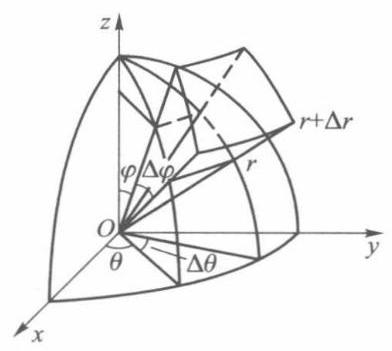
\includegraphics[width=.3\textwidth]{images/P192.jpg}
	\caption{图 $21-37$}
	\label{fig:P192}
\end{figure}

\begin{figure}
	\centering
	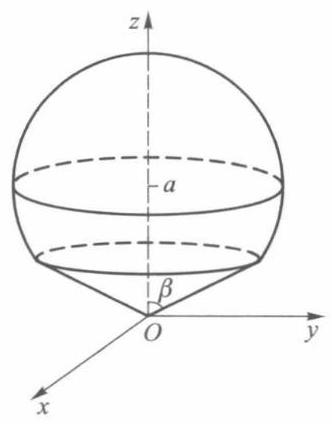
\includegraphics[width=.3\textwidth]{images/P193.jpg}
	\caption{图 $21-38$}
	\label{fig:P193}
\end{figure}

%解
\begin{solution}

\end{solution}
在球坐标变换下,球面方程 \({x}^{2} + {y}^{2} + {\left( z - a\right) }^{2} = {a}^{2}\) 可表示成 \(r = {2a}\cos \varphi\) ,锥面方程 \(z = \sqrt{{x}^{2} + {y}^{2}}\cot \beta\) 可表示成 \(\varphi  = \beta\) . 因此
\[
{V}^{\prime } = \{ \left( {r,\varphi ,\theta }\right)  \mid  0 \leq  r \leq  {2a}\cos \varphi ,0 \leq  \varphi  \leq  \beta ,0 \leq  \theta  \leq  {2\pi }\} .
\]
由公式 (7) 求得 \(V\) 的体积为
\[
{\iiint }_{V}\mathrm{\;d}V = {\int }_{0}^{2\pi }\mathrm{d}\theta {\int }_{0}^{\beta }\mathrm{d}\varphi {\int }_{0}^{{2a}\cos \varphi }{r}^{2}\sin \varphi \mathrm{d}r = \frac{4}{3}\pi {a}^{3}\left( {1 - {\cos }^{4}\beta }\right) .
\]
除上述介绍的两种变换外, 下面我们再举一个例子, 进一步说明如何根据被积函数或积分区域的特点来选择其他不同的变换.

%例 6
\begin{example}

\end{example}
求 \(I = {\iiint }_{V}z\mathrm{\;d}x\mathrm{\;d}y\mathrm{\;d}z\) ,其中 \(V\) 为由 \(\frac{{x}^{2}}{{a}^{2}} + \frac{{y}^{2}}{{b}^{2}} + \frac{{z}^{2}}{{c}^{2}} \leq  1\) 与 \(z \geq  0\) 所交区域.

%解
\begin{solution}

\end{solution}
作广义球坐标变换
\[
T : \left\{  \begin{array}{l} x = {ar}\sin \varphi \cos \theta , \\  y = {br}\sin \varphi \sin \theta , \\  z = {cr}\cos \varphi , \end{array}\right.
\]
于是 \(J = {abc}{r}^{2}\sin \varphi\) . 在上述广义球坐标变换下, \(V\) 的原象为
\[
{V}^{\prime } = \left\{  {\left( {r,\varphi ,\theta }\right)  \mid  0 \leq  r \leq  1,0 \leq  \varphi  \leq  \frac{\pi }{2},0 \leq  \theta  \leq  {2\pi }}\right\}  .
\]
由公式 (7), 有
\[
{\iiint }_{V}z\mathrm{\;d}x\mathrm{\;d}y\mathrm{\;d}z = {\iiint }_{{V}^{\prime }}{ab}{c}^{2}{r}^{3}\sin \varphi \cos \varphi \mathrm{d}r\mathrm{\;d}\varphi \mathrm{d}\theta
\]
\[
= {\int }_{0}^{2\pi }\mathrm{d}\theta {\int }_{0}^{\frac{\pi }{2}}\mathrm{\;d}\varphi {\int }_{0}^{1}{ab}{c}^{2}{r}^{3}\sin \varphi \cos \varphi \mathrm{d}r
\]
\[
= \frac{{\pi ab}{c}^{2}}{2}{\int }_{0}^{\frac{\pi }{2}}\sin \varphi \cos \varphi \mathrm{d}\varphi  = \frac{{\pi ab}{c}^{2}}{4}\text{ . }
\]
\subsection{习题 21.5}

1. 计算下列积分:

(1) \({\iiint }_{V}\left( {{xy} + {z}^{2}}\right) \mathrm{d}x\mathrm{\;d}y\mathrm{\;d}z\) ,其中 \(V = \left\lbrack  {-2,5}\right\rbrack   \times  \left\lbrack  {-3,3}\right\rbrack   \times  \left\lbrack  {0,1}\right\rbrack\) ；

(2) \({\iiint }_{V}x\cos y\cos z\mathrm{\;d}x\mathrm{\;d}y\mathrm{\;d}z\) ,其中 \(V = \left\lbrack  {0,1}\right\rbrack   \times  \left\lbrack  {0,\frac{\pi }{2}}\right\rbrack   \times  \left\lbrack  {0,\frac{\pi }{2}}\right\rbrack\) ；

( 3 ) \({\iint }_{V}\frac{\mathrm{d}x\mathrm{\;d}y\mathrm{\;d}z}{{\left( 1 + x + y + z\right) }^{3}}\) ,其中 \(V\) 是由 \(x + y + z = 1\) 与三个坐标面所围成的区域；

(4) \({\iiint }_{V}y\cos \left( {x + z}\right) \mathrm{d}x\mathrm{\;d}y\mathrm{\;d}z\) ,其中 \(V\) 是由 \(y = \sqrt{x},y = 0,z = 0\) 及 \(x + z = \frac{\pi }{2}\) 所围成的区域.

2. 试改变下列累次积分的顺序:

(1) \({\int }_{0}^{1}\mathrm{\;d}x{\int }_{0}^{1 - x}\mathrm{\;d}y{\int }_{0}^{x + y}f\left( {x,y,z}\right) \mathrm{d}z\) ;

(2) \({\int }_{0}^{1}\mathrm{\;d}x{\int }_{0}^{1}\mathrm{\;d}y{\int }_{0}^{{x}^{2} + {y}^{2}}f\left( {x,y,z}\right) \mathrm{d}z\) .

3. 计算下列三重积分与累次积分:

(1) \({\iiint }_{V}{z}^{2}\mathrm{\;d}x\mathrm{\;d}y\mathrm{\;d}z\) ,其中 \(V\) 由 \({x}^{2} + {y}^{2} + {z}^{2} \leq  {r}^{2}\) 和 \({x}^{2} + {y}^{2} + {z}^{2} \leq  {2rz}\) 所确定；

(2) \({\int }_{0}^{1}\mathrm{\;d}x{\int }_{0}^{\sqrt{1 - {x}^{2}}}\mathrm{\;d}y{\int }_{\sqrt{{x}^{2} + {y}^{2}}}^{\sqrt{2 - {x}^{2} - {y}^{2}}}{z}^{2}\mathrm{\;d}z\) .

4. 利用适当的坐标变换,计算下列各曲面所围成的体积:

(1) \(z = {x}^{2} + {y}^{2},z = 2\left( {{x}^{2} + {y}^{2}}\right) ,y = x,y = {x}^{2}\) ;

(2) \({\left( \frac{x}{a} + \frac{y}{b}\right) }^{2} + {\left( \frac{z}{c}\right) }^{2} = 1\;\left( {x \geq  0,y \geq  0,z \geq  0,a > 0,b > 0,c > 0}\right)\) .

5. 设球体 \({x}^{2} + {y}^{2} + {z}^{2} \leq  {2x}\) 上各点的密度等于该点到坐标原点的距离,求该球体的质量.

6. 证明定理 21.16 及其推论.

7. 设 \(V = \left\{  {\left( {x,y,z}\right) \left| {\;\frac{{x}^{2}}{{a}^{2}} + \frac{{y}^{2}}{{b}^{2}} + \frac{{z}^{2}}{{c}^{2}} \leq  1}\right. }\right\}\) ,计算下列积分:

(1) \(\iiint \sqrt{1 - \frac{{x}^{2}}{{a}^{2}} - \frac{{y}^{2}}{{b}^{2}} - \frac{{z}^{2}}{{c}^{2}}}\mathrm{d}x\mathrm{\;d}y\mathrm{\;d}z\) ；

(2) \({\iiint }_{V}{\mathrm{e}}^{\sqrt{\frac{{x}^{2}}{{a}^{2}} + \frac{{y}^{2}}{{b}^{2}} + \frac{{z}^{2}}{{c}^{2}}}}\mathrm{d}x\mathrm{\;d}y\mathrm{\;d}z\) .

\section{重积分的应用}

重积分的应用除前面提到的可用以求空间立体的体积及空间物体的质量外, 这里再举几个它在几何与力学方面的应用.

\subsection{曲面的面积}

设 \(D\) 为可求面积的平面有界区域,函数 \(f\left( {x,y}\right)\) 在 \(D\) 上具有连续的一阶偏导数,讨论由方程
\[
z = f\left( {x,y}\right) ,\left( {x,y}\right)  \in  D
\]
所确定的曲面 \(S\) 的面积.

\begin{figure}
	\centering
	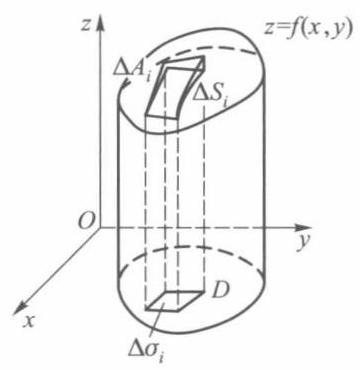
\includegraphics[width=.3\textwidth]{images/P194.jpg}
	\caption{图 $21-39$}
	\label{fig:P194}
\end{figure}

为了定义曲面 \(S\) 的面积,对区域 \(D\) 作分割 \(T\) ,它把 \(D\) 分成 \(n\) 个小区域 \({\sigma }_{i}\left( {i = 1,2,\cdots ,n}\right)\) . 根据这个分割相应地将曲面 \(S\) 也分成 \(n\) 个小曲面片 \({S}_{i}\left( {i = 1,2,\cdots ,n}\right)\) . 在每个 \({S}_{i}\) 上任取一点 \({M}_{i}\) ,作曲面在这一点的切平面 \({\pi }_{i}\) ,并在 \({\pi }_{i}\) 上取出一小块 \({A}_{i}\) ,使得 \({A}_{i}\) 与 \({S}_{i}\) 在 \({xy}\) 平面上的投影都是 \({\sigma }_{i}\) , 如图 21-39 所示. 现在点 \({M}_{i}\) 附近,用切平面 \({A}_{i}\) 代替小曲面片 \({S}_{i}\) ,从而当 \(\parallel T\parallel\) 充分小时,有
\[
{\Delta S} = \mathop{\sum }\limits_{{i = 1}}^{n}\Delta {S}_{i} \approx  \mathop{\sum }\limits_{{i = 1}}^{n}\Delta {A}_{i},
\]
这里 \({\Delta S},\Delta {S}_{i},\Delta {A}_{i}\) 分别表示曲面 \(S\) ,小曲面片 \({S}_{i}\) ,小切平面块 \({A}_{i}\) 的面积. 所以当 \(\parallel T\parallel  \rightarrow\) 0 时,可用和式 \(\mathop{\sum }\limits_{{i = 1}}^{n}\Delta {A}_{i}\) 的极限作为 \(S\) 的面积.

现在按照上述给出的曲面面积的概念, 来建立曲面面积的计算公式.

首先计算 \({A}_{i}\) 的面积. 由于切平面 \({\pi }_{i}\) 的法向量就是曲面 \(S\) 在点 \({M}_{i}\left( {{\xi }_{i},{\eta }_{i},{\zeta }_{i}}\right)\) 处的法向量,记它与 \(z\) 轴的夹角为 \({\gamma }_{i}\) ,则
\[
\left| {\cos {\gamma }_{i}}\right|  = \frac{1}{\sqrt{1 + {f}_{x}^{2}\left( {{\xi }_{i},{\eta }_{i}}\right)  + {f}_{y}^{2}\left( {{\xi }_{i},{\eta }_{i}}\right) }}.
\]
因为 \({A}_{i}\) 在 \({xy}\) 平面上的投影为 \({\sigma }_{i}\) ,所以
\[
\Delta {A}_{i} = \frac{\Delta {\sigma }_{i}}{\left| \cos {\gamma }_{i}\right| } = \sqrt{1 + {f}_{x}^{2}\left( {{\xi }_{i},{\eta }_{i}}\right)  + {f}_{y}^{2}\left( {{\xi }_{i},{\eta }_{i}}\right) }\Delta {\sigma }_{i}.
\]
其次, 由于和数
\[
\mathop{\sum }\limits_{{i = 1}}^{n}\Delta {A}_{i} = \mathop{\sum }\limits_{{i = 1}}^{n}\sqrt{1 + {f}_{x}^{2}\left( {{\xi }_{i},{\eta }_{i}}\right)  + {f}_{y}^{2}\left( {{\xi }_{i},{\eta }_{i}}\right) }\Delta {\sigma }_{i}
\]
是连续函数 \(\sqrt{1 + {f}_{x}^{2}\left( {x,y}\right)  + {f}_{y}^{2}\left( {x,y}\right) }\) 在有界闭区域 \(D\) 上的积分和. 于是当 \(\parallel T\parallel  \rightarrow  0\) 时,就得到
\[
{\Delta S} = \mathop{\lim }\limits_{{\parallel T\parallel  \rightarrow  0}}\mathop{\sum }\limits_{{i = 1}}^{n}\sqrt{1 + {f}_{x}^{2}\left( {{\xi }_{i},{\eta }_{i}}\right)  + {f}_{y}^{2}\left( {{\xi }_{i},{\eta }_{i}}\right) }\Delta {\sigma }_{i}
\]
\[
= {\iint }_{D}\sqrt{1 + {f}_{x}^{2}\left( {x,y}\right)  + {f}_{y}^{2}\left( {x,y}\right) }\mathrm{d}x\mathrm{\;d}y \tag{1}
\]
或
\[
{\Delta S} = \mathop{\lim }\limits_{{\parallel T\parallel  \rightarrow  0}}\mathop{\sum }\limits_{{i = 1}}^{n}\frac{\Delta {\sigma }_{i}}{\left| \cos {\gamma }_{i}\right| } = {\iint }_{D}\frac{\mathrm{d}x\mathrm{\;d}y}{\left| \overset{⏜}{\cos \left( {\mathbf{n},z}\right) }\right| }, \tag{2}
\]
其中 \(\cos \left( {\mathbf{n},z}\right)\) 为曲面的法向量 \(\mathbf{n}\) 与 \(z\) 轴正向夹角的余弦.

%例 1
\begin{example}

\end{example}
求圆锥 \(z = \sqrt{{x}^{2} + {y}^{2}}\) 在圆柱体 \({x}^{2} + {y}^{2} \leq  x\) 内那一部分的面积.

%解
\begin{solution}

\end{solution}
据曲面面积公式 (1),
\[
{\Delta S} = {\iint }_{D}\sqrt{1 + {z}_{x}^{2} + {z}_{y}^{2}}\mathrm{\;d}x\mathrm{\;d}y,
\]
其中 \(D\) 是 \({x}^{2} + {y}^{2} \leq  x\) . 所求曲面方程为
\[
z = \sqrt{{x}^{2} + {y}^{2}},
\]
故
\[
{z}_{x} = \frac{x}{\sqrt{{x}^{2} + {y}^{2}}},{z}_{y} = \frac{y}{\sqrt{{x}^{2} + {y}^{2}}}.
\]
因此
\[
\sqrt{1 + {z}_{x}^{2} + {z}_{y}^{2}} = \sqrt{1 + \frac{{x}^{2}}{{x}^{2} + {y}^{2}} + \frac{{y}^{2}}{{x}^{2} + {y}^{2}}} = \sqrt{2},
\]
所以
\[
{\Delta S} = {\iint }_{D}\sqrt{2}\mathrm{\;d}x\mathrm{\;d}y = \sqrt{2}{\Delta D} = \frac{\sqrt{2}}{4}\pi .
\]
在上册的定积分应用中, 曾用微元法给出过旋转面的面积公式, 下面用二重积分给予严格证明.

%例 2
\begin{example}

\end{example}
设平面光滑曲线的方程为
\[
y = f\left( x\right) ,x \in  \left\lbrack  {a,b}\right\rbrack  \left( {f\left( x\right)  > 0}\right) ,
\]
求证: 此曲线绕 \(x\) 轴旋转一周得到的旋转曲面的面积为
\[
S = {2\pi }{\int }_{a}^{b}f\left( x\right) \sqrt{1 + {f}^{\prime 2}\left( x\right) }\mathrm{d}x.
\]
%证
\begin{proof}

\end{proof}
由于上半旋转面方程为 \(z = \sqrt{{f}^{2}\left( x\right)  - {y}^{2}}\) ,因此
\[
{z}_{x} = \frac{f\left( x\right) {f}^{\prime }\left( x\right) }{\sqrt{{f}^{2}\left( x\right)  - {y}^{2}}},{z}_{y} = \frac{-y}{\sqrt{{f}^{2}\left( x\right)  - {y}^{2}}},
\]
\[
\sqrt{1 + {z}_{x}^{2} + {z}_{y}^{2}} = \sqrt{\frac{{f}^{2}\left( x\right)  + {f}^{2}\left( x\right) {f}^{\prime 2}\left( x\right) }{{f}^{2}\left( x\right)  - {y}^{2}}},
\]
于是
\[
S = 2{\int }_{a}^{b}\mathrm{\;d}x{\int }_{-f\left( x\right) }^{f\left( x\right) }\sqrt{\frac{{f}^{2}\left( x\right)  + {f}^{2}\left( x\right) {f}^{\prime 2}\left( x\right) }{{f}^{2}\left( x\right)  - {y}^{2}}}\mathrm{\;d}y
\]
\[
= 4{\int }_{a}^{b}\mathrm{\;d}x{\int }_{0}^{f\left( x\right) }f\left( x\right) \sqrt{\frac{1 + {f}^{\prime 2}\left( x\right) }{1 - {y}^{2}{f}^{-2}\left( x\right) }}\mathrm{d}\left( \frac{y}{f\left( x\right) }\right)
\]
\[
= 4{\int }_{a}^{b}f\left( x\right) \sqrt{1 + {f}^{\prime 2}\left( x\right) }\mathrm{d}x{\int }_{0}^{1}\frac{\mathrm{d}t}{\sqrt{1 - {t}^{2}}}
\]
\[
= {2\pi }{\int }_{a}^{b}f\left( x\right) \sqrt{1 + {f}^{\prime 2}\left( x\right) }\mathrm{d}x.
\]
若空间曲面 \(S\) 由参量方程
\[
x = x\left( {u,v}\right) ,y = y\left( {u,v}\right) ,z = z\left( {u,v}\right) ,\left( {u,v}\right)  \in  {D}^{\prime } \tag{3}
\]
确定,其中 \(x\left( {u,v}\right) ,y\left( {u,v}\right) ,z\left( {u,v}\right)\) 在 \({D}^{\prime }\) 上具有连续的一阶偏导数,且
\[
\frac{\partial \left( {x,y}\right) }{\partial \left( {u,v}\right) },\;\frac{\partial \left( {y,z}\right) }{\partial \left( {u,v}\right) },\;\frac{\partial \left( {z,x}\right) }{\partial \left( {u,v}\right) }
\]
中至少有一个不等于零,则曲面 \(S\) 在点(x, y, z)的法线方向数为
\[
\left( {\frac{\partial \left( {y,z}\right) }{\partial \left( {u,v}\right) },\frac{\partial \left( {z,x}\right) }{\partial \left( {u,v}\right) },\frac{\partial \left( {x,y}\right) }{\partial \left( {u,v}\right) }}\right) ,
\]
它与 \(z\) 轴的夹角的余弦的绝对值为
\[
\left| {\cos \left( {\widehat{n},z}\right) }\right|  = \left| \frac{\frac{\partial \left( {x,y}\right) }{\partial \left( {u,v}\right) }}{\sqrt{{\left( \frac{\partial \left( {y,z}\right) }{\partial \left( {u,v}\right) }\right) }^{2} + {\left( \frac{\partial \left( {z,x}\right) }{\partial \left( {u,v}\right) }\right) }^{2} + {\left( \frac{\partial \left( {x,y}\right) }{\partial \left( {u,v}\right) }\right) }^{2}}}\right|
\]
\[
= \left| \frac{\frac{\partial \left( {x,y}\right) }{\partial \left( {u,v}\right) }}{\sqrt{\left( {{x}_{u}^{2} + {y}_{u}^{2} + {z}_{u}^{2}}\right) \left( {{x}_{v}^{2} + {y}_{v}^{2} + {z}_{v}^{2}}\right)  - {\left( {x}_{u}{x}_{v} + {y}_{u}{y}_{v} + {z}_{u}{z}_{v}\right) }^{2}}}\right|
\]
\[
= \left| \frac{\partial \left( {x,y}\right) }{\partial \left( {u,v}\right) }\right| \frac{1}{\sqrt{{EG} - {F}^{2}}}, \tag{4}
\]
其中
\[
E = {x}_{u}^{2} + {y}_{u}^{2} + {z}_{u}^{2},
\]
\[
F = {x}_{u}{x}_{v} + {y}_{u}{y}_{v} + {z}_{u}{z}_{v},
\]
\[
G = {x}_{v}^{2} + {y}_{v}^{2} + {z}_{v}^{2}.
\]
当 \(\frac{\partial \left( {x,y}\right) }{\partial \left( {u,v}\right) } \neq  0\) 时,对(2)作变换 \(x = x\left( {u,v}\right) ,y = y\left( {u,v}\right)\) ,则有
\[
{\Delta S} = {\iint }_{D}\frac{1}{\left| \cos \left( \mathbf{n},z\right) \right| }\mathrm{d}x\mathrm{\;d}y
\]
\[
= {\iint }_{{D}^{\prime }}\frac{1}{\left| \overset{⏜}{\cos \left( {\mathbf{n},z}\right) }\right| }\left| \frac{\partial \left( {x,y}\right) }{\partial \left( {u,v}\right) }\right| \mathrm{d}u\mathrm{\;d}v.
\]
由 (4), 得到由参量方程 (3) 所表示的曲面面积公式:
\[
{\Delta S} = {\iint }_{{D}^{\prime }}\sqrt{{EG} - {F}^{2}}\mathrm{\;d}u\mathrm{\;d}v. \tag{5}
\]
\begin{figure}
	\centering
	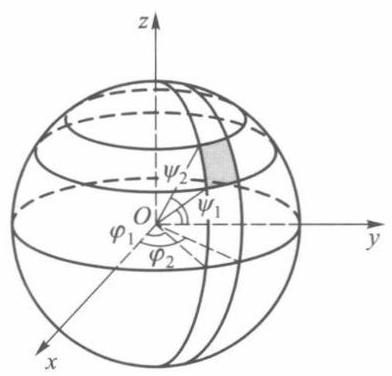
\includegraphics[width=.3\textwidth]{images/P195.jpg}
	\caption{图 $21-40$}
	\label{fig:P195}
\end{figure}

%例 3
\begin{example}

\end{example}
求球面上两条纬线和两条经线之间的曲面的面积 (图 21-40 中阴影部分).

%解
\begin{solution}

\end{solution}
设球面方程为
\[
x = R\cos \psi \cos \varphi ,
\]
\[
y = R\cos \psi \sin \varphi ,
\]
\[
z = R\sin \psi ,
\]
其中 \(R\) 为球的半径. 本例是求当 \({\varphi }_{1} \leq  \varphi  \leq  {\varphi }_{2},{\psi }_{1} \leq  \psi  \leq  {\psi }_{2}\) 时的球面部分面积. 由于
\[
E = {x}_{\psi }^{2} + {y}_{\psi }^{2} + {z}_{\psi }^{2} = {R}^{2},
\]
\[
F = 0,G = {R}^{2}{\cos }^{2}\psi ,
\]
所以
\[
\sqrt{{EG} - {F}^{2}} = {R}^{2}\cos \psi .
\]
由公式 (5) 即得所求曲面的面积.
\[
{\Delta S} = {\int }_{{\varphi }_{1}}^{{\varphi }_{2}}\mathrm{\;d}\varphi {\int }_{{\psi }_{1}}^{{\psi }_{2}}{R}^{2}\cos \psi \mathrm{d}\psi  = {R}^{2}\left( {{\varphi }_{2} - {\varphi }_{1}}\right) \left( {\sin {\psi }_{2} - \sin {\psi }_{1}}\right) .
\]
在讨论曲线弧长时, 我们曾用弧内接折线的长在其各段的长趋于零时的极限来定义. 但是能否类似地用曲面的内接多面形的面积, 在其各个面积的直径趋于零时的极限来定义呢? 施瓦茨 (Schwarz) 曾举出一个反例说明这样的定义方法是不可行的. 对此读者可参见有关的数学分析教程 (如菲赫金哥尔茨《微积分学教程》中译本第三卷第二分册).

\subsection{质心}

设 \(V\) 是密度函数为 \(\rho \left( {x,y,z}\right)\) 的空间物体, \(\rho \left( {x,y,z}\right)\) 在 \(V\) 上连续. 为求得 \(V\) 的质心坐标公式,先对 \(V\) 作分割 \(T\) ,在属于分割 \(T\) 的每一小块 \({v}_{i}\) 上任取一点 \(\left( {{\xi }_{i},{\eta }_{i},{\zeta }_{i}}\right)\) ,于是小块 \({v}_{i}\) 的质量可以 \(\rho \left( {{\xi }_{i},{\eta }_{i},{\zeta }_{i}}\right) \Delta {v}_{i}\) 近似代替. 若把每一小块看作质量集中在 \(\left( {{\xi }_{i},{\eta }_{i},{\zeta }_{i}}\right)\) 的质点时,整个物体就可用这 \(n\) 个质点的质点系来近似代替. 由于质点系的质心坐标公式为
\[
{\bar{x}}_{n} = \frac{\mathop{\sum }\limits_{{i = 1}}^{n}{\xi }_{i}\rho \left( {{\xi }_{i},{\eta }_{i},{\zeta }_{i}}\right) \Delta {v}_{i}}{\mathop{\sum }\limits_{{i = 1}}^{n}\rho \left( {{\xi }_{i},{\eta }_{i},{\zeta }_{i}}\right) \Delta {v}_{i}},\;{\bar{y}}_{n} = \frac{\mathop{\sum }\limits_{{i = 1}}^{n}{\eta }_{i}\rho \left( {{\xi }_{i},{\eta }_{i},{\zeta }_{i}}\right) \Delta {v}_{i}}{\mathop{\sum }\limits_{{i = 1}}^{n}\rho \left( {{\xi }_{i},{\eta }_{i},{\zeta }_{i}}\right) \Delta {v}_{i}},\;{\bar{z}}_{n} = \frac{\mathop{\sum }\limits_{{i = 1}}^{n}{\zeta }_{i}\rho \left( {{\xi }_{i},{\eta }_{i},{\zeta }_{i}}\right) \Delta {v}_{i}}{\mathop{\sum }\limits_{{i = 1}}^{n}\rho \left( {{\xi }_{i},{\eta }_{i},{\zeta }_{i}}\right) \Delta {v}_{i}}.
\]
当 \(\parallel T\parallel  \rightarrow  0\) 时,我们很自然地把 \({\bar{x}}_{n},{\bar{y}}_{n},{\bar{z}}_{n}\) 的极限 \(\bar{x},\bar{y},\bar{z}\) 定义为 \(V\) 的质心坐标,即
\[
\bar{x} = \frac{{\iint }_{V}{x\rho }\left( {x,y,z}\right) \mathrm{d}V}{{\iiint }_{V}\rho \left( {x,y,z}\right) \mathrm{d}V},\;\bar{y} = \frac{{\iint }_{V}{y\rho }\left( {x,y,z}\right) \mathrm{d}V}{{\iiint }_{V}\rho \left( {x,y,z}\right) \mathrm{d}V},\;\bar{z} = \frac{{\iiint }_{V}{z\rho }\left( {x,y,z}\right) \mathrm{d}V}{{\iiint }_{V}\rho \left( {x,y,z}\right) \mathrm{d}V}.
\]
当物体 \(V\) 的密度均匀即 \(\rho\) 为常数时,则有
\[
\bar{x} = \frac{1}{\Delta V}{\iiint }_{V}x\mathrm{\;d}V,\;\bar{y} = \frac{1}{\Delta V}{\iiint }_{V}y\mathrm{\;d}V,\;\bar{z} = \frac{1}{\Delta V}{\iiint }_{V}z\mathrm{\;d}V,
\]
这里 \({\Delta V}\) 为 \(V\) 的体积.

读者同样可以得到,密度分布为 \(\rho \left( {x,y}\right)\) 的平面薄板 \(D\) 的质心坐标是
\[
\bar{x} = \frac{{\iint }_{D}{x\rho }\left( {x,y}\right) \mathrm{d}\sigma }{{\iint }_{D}\rho \left( {x,y}\right) \mathrm{d}\sigma },\;\bar{y} = \frac{{\iint }_{D}{y\rho }\left( {x,y}\right) \mathrm{d}\sigma }{{\iint }_{D}\rho \left( {x,y}\right) \mathrm{d}\sigma }.
\]
当平面薄板 \(D\) 的密度均匀时,即 \(\rho\) 是常数时,则有
\[
\bar{x} = \frac{1}{\Delta D}{\iint }_{D}x\mathrm{\;d}\sigma ,\;\bar{y} = \frac{1}{\Delta D}{\iint }_{D}y\mathrm{\;d}\sigma ,
\]
这里 \({\Delta D}\) 为平面薄板 \(D\) 的面积.

%例 4
\begin{example}

\end{example}
求密度均匀的上半椭球体的质心.

%解
\begin{solution}

\end{solution}
设椭球体由不等式
\[
\frac{{x}^{2}}{{a}^{2}} + \frac{{y}^{2}}{{b}^{2}} + \frac{{z}^{2}}{{c}^{2}} \leq  1
\]
表示. 由对称性知 \(\bar{x} = 0,\bar{y} = 0\) . 又由 \(\rho\) 为常数,所以
\[
\bar{z} = \frac{{\iiint }_{V}{\rho z}\mathrm{\;d}V}{{\iiint }_{V}\rho \mathrm{d}V} = \frac{{\iiint }_{V}z\mathrm{\;d}x\mathrm{\;d}y\mathrm{\;d}z}{\frac{2}{3}{\pi abc}}.
\]
由 §5 例 6 得
\[
\bar{z} = \frac{3c}{8}.
\]
\subsection{转动惯量}

质点 \(A\) 对于轴 \(l\) 的转动惯量 \(J\) 是质点 \(A\) 的质量 \(m\) 和 \(A\) 与转动轴 \(l\) 的距离 \(r\) 的平方的乘积,即 \(J = m{r}^{2}\) .

现在讨论空间物体 \(V\) 的转动惯量问题. 我们仍然采用第二段中的办法,把 \(V\) 看作由 \(n\) 个质点组成的质点系,然后用取极限的方法求得 \(V\) 的转动惯量.

设 \(\rho \left( {x,y,z}\right)\) 为空间物体 \(V\) 的密度分布函数,它在 \(V\) 上连续. 对 \(V\) 作分割 \(T\) ,在属于 \(T\) 的每一小块 \({v}_{i}\) 上任取一点 \(\left( {{\xi }_{i},{\eta }_{i},{\zeta }_{i}}\right)\) ,于是 \({v}_{i}\) 的质量可以 \(\rho \left( {{\xi }_{i},{\eta }_{i},{\zeta }_{i}}\right) \Delta {v}_{i}\) 近似替代. 当以质点系 \(\left\{  {\left( {{\xi }_{i},{\eta }_{i},{\zeta }_{i}}\right) ,i = 1,2,\cdots ,n}\right\}\) 近似替代 \(V\) 时,质点系对于 \(x\) 轴的转动惯量则是
\[
{J}_{{x}_{n}} = \mathop{\sum }\limits_{{i = 1}}^{n}\left( {{\eta }_{i}^{2} + {\zeta }_{i}^{2}}\right) \rho \left( {{\xi }_{i},{\eta }_{i},{\zeta }_{i}}\right) \Delta {v}_{i}.
\]
当 \(\parallel T\parallel  \rightarrow  0\) 时,上述积分和的极限就是物体 \(V\) 对于 \(x\) 轴的转动惯量
\[
{J}_{x} = {\iiint }_{V}\left( {{y}^{2} + {z}^{2}}\right) \rho \left( {x,y,z}\right) \mathrm{d}V.
\]
类似可得物体 \(V\) 对于 \(y\) 轴与 \(z\) 轴的转动惯量分别为
\[
{J}_{y} = {\iiint }_{V}\left( {{z}^{2} + {x}^{2}}\right) \rho \left( {x,y,z}\right) \mathrm{d}V,
\]
\[
{J}_{z} = {\iiint }_{V}\left( {{x}^{2} + {y}^{2}}\right) \rho \left( {x,y,z}\right) \mathrm{d}V.
\]
同理,物体 \(V\) 对于坐标平面的转动惯量分别为
\[
{J}_{xy} = {\iiint }_{V}{z}^{2}\rho \left( {x,y,z}\right) \mathrm{d}V,
\]
\[
{J}_{yz} = {\iiint }_{V}{x}^{2}\rho \left( {x,y,z}\right) \mathrm{d}V,
\]
\[
{J}_{zx} = {\iiint }_{V}^{2}\rho \left( {x,y,z}\right) \mathrm{d}V.
\]
据此, 读者也容易建立平面薄板对于坐标轴的转动惯量:
\[
{J}_{x} = {\iint }_{D}{y}^{2}\rho \left( {x,y}\right) \mathrm{d}\sigma ,\;{J}_{y} = {\iint }_{D}{x}^{2}\rho \left( {x,y}\right) \mathrm{d}\sigma
\]
以及
\[
{J}_{l} = {\iint }_{D}{r}^{2}\left( {x,y}\right) \rho \left( {x,y}\right) \mathrm{d}\sigma ,
\]
这里 \(l\) 为转动轴, \(r\left( {x,y}\right)\) 为 \(D\) 中点(x, y)到 \(l\) 的距离函数.

%例 5
\begin{example}

\end{example}
求密度均匀的圆环 \(D\) 对于垂直于圆环面中心轴的转动惯量 (图21-41).

\begin{center}

\includegraphics[width=.3\textwidth]{images/P196.jpg}
\end{center}


%解
\begin{solution}

\end{solution}
设圆环 \(D\) 为
\[
{R}_{1}^{2} \leq  {x}^{2} + {y}^{2} \leq  {R}_{2}^{2},
\]
密度为 \(\rho\) ,则 \(D\) 中任一点(x, y)与转轴的距离平方为 \({x}^{2} + {y}^{2}\) . 于是转动惯量
\[
J = {\iint }_{D}\rho \left( {{x}^{2} + {y}^{2}}\right) \mathrm{d}\sigma  = \rho {\int }_{0}^{2\pi }\mathrm{d}\theta {\int }_{{R}_{1}}^{{R}_{2}}{r}^{3}\mathrm{\;d}r
\]
\[
= \frac{\pi \rho }{2}\left( {{R}_{2}^{4} - {R}_{1}^{4}}\right)  = \frac{m}{2}\left( {{R}_{2}^{2} + {R}_{1}^{2}}\right) ,
\]
其中 \(m\) 为圆环的质量.

%例 6
\begin{example}

\end{example}
求均匀圆盘 \(D\) 对于其直径的转动惯量 (图 21-42).

%解
\begin{solution}

\end{solution}
设圆盘 \(D\) 为 \({x}^{2} + {y}^{2} \leq  {R}^{2}\) ,密度为 \(\rho\) ,求对于 \(y\) 轴的转动惯量. 由于 \(D\) 内任一点 (x, y)与 \(y\) 轴的距离为 \(\left| x\right|\) ,故
\[
J = {\iint }_{D}\rho {x}^{2}\mathrm{\;d}\sigma  = \rho {\int }_{0}^{2\pi }\mathrm{d}\theta {\int }_{0}^{R}{\left( r\cos \theta \right) }^{2}r\mathrm{\;d}r
\]
\[
= \rho {\int }_{0}^{2\pi }{\cos }^{2}\theta \mathrm{d}\theta {\int }_{0}^{R}{r}^{3}\mathrm{\;d}r
\]
\[
= \frac{{\rho \pi }{R}^{4}}{4} = \frac{1}{4}m{R}^{2},
\]
其中 \(m\) 为圆盘的质量.

\begin{figure}
	\centering
	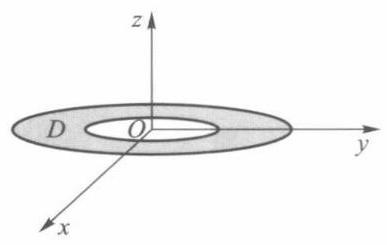
\includegraphics[width=.3\textwidth]{images/P197.jpg}
	\caption{图 $21-41$}
	\label{fig:P197}
\end{figure}

\begin{figure}
	\centering
	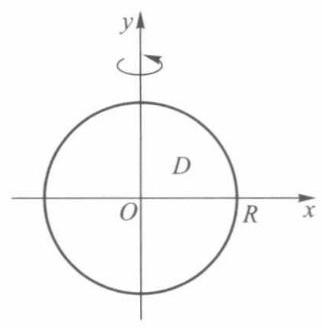
\includegraphics[width=.3\textwidth]{images/P198.jpg}
	\caption{图 $21-42$}
	\label{fig:P198}
\end{figure}

%例 7
\begin{example}

\end{example}
设某球体的密度与球心的距离成正比, 求它对于切平面的转动惯量.

%解
\begin{solution}

\end{solution}
设球体由不等式 \({x}^{2} + {y}^{2} + {z}^{2} \leq  {R}^{2}\) 表示,密度函数为 \(k\sqrt{{x}^{2} + {y}^{2} + {z}^{2}}\) ,这里 \(k\) 为比例常数. 切平面方程为 \(x = R\) ,则球体对于平面 \(x = R\) 的转动惯量为
\[
J = k{\iiint }_{V}\sqrt{{x}^{2} + {y}^{2} + {z}^{2}}{\left( R - x\right) }^{2}\mathrm{\;d}x\mathrm{\;d}y\mathrm{\;d}z
\]
\[
= k{\int }_{0}^{2\pi }\mathrm{d}\theta {\int }_{0}^{\pi }\mathrm{d}\varphi {\int }_{0}^{R}{\left( R - r\sin \varphi \cos \theta \right) }^{2}{r}^{3}\sin \varphi \mathrm{d}r
\]
\[
= k{R}^{2}{\int }_{0}^{2\pi }\mathrm{d}\theta {\int }_{0}^{R}{r}^{3}\mathrm{\;d}r{\int }_{0}^{\pi }\sin \varphi \mathrm{d}\varphi  - {2kR}{\int }_{0}^{2\pi }\cos \theta \mathrm{d}\theta {\int }_{0}^{R}{r}^{4}\mathrm{\;d}r{\int }_{0}^{\pi }{\sin }^{2}\varphi \mathrm{d}\varphi  +
\]
\[
k{\int }_{0}^{2\pi }{\cos }^{2}\theta \mathrm{d}\theta {\int }_{0}^{R}{r}^{5}\mathrm{\;d}r{\int }_{0}^{\pi }{\sin }^{3}\varphi \mathrm{d}\varphi
\]
\[
= \frac{11}{9}{k\pi }{R}^{6}\text{ . }
\]


\subsection{引力}

求密度为 \(\rho \left( {x,y,z}\right)\) 的立体对立体外质量为 1 的质点 \(A\) 的引力.

设 \(A\) 的坐标为 \(\left( {\xi ,\eta ,\zeta }\right) ,V\) 中点的坐标用(x, y, z)表示. 我们使用微元法来求 \(V\) 对 \(A\) 的引力. \(V\) 中质量微元 \(\mathrm{d}m = \rho \mathrm{d}V\) 对 \(A\) 的引力在坐标轴上的投影为
\[
\mathrm{d}{F}_{x} = k\frac{x - \xi }{{r}^{3}}\rho \mathrm{d}V,\mathrm{\;d}{F}_{y} = k\frac{y - \eta }{{r}^{3}}\rho \mathrm{d}V,\mathrm{\;d}{F}_{z} = k\frac{z - \zeta }{{r}^{3}}\rho \mathrm{d}V,
\]
其中 \(k\) 为引力系数,
\[
r = \sqrt{{\left( x - \xi \right) }^{2} + {\left( y - \eta \right) }^{2} + {\left( z - \zeta \right) }^{2}}
\]
是 \(A\) 到 \(\mathrm{d}V\) 的距离,于是力 \(\mathbf{F}\) 在三个坐标轴上的投影分别为
\[
{F}_{x} = k{\iiint }_{V}\frac{x - \xi }{{r}^{3}}\rho \mathrm{d}V,\;{F}_{y} = k{\iiint }_{V}\frac{y - \eta }{{r}^{3}}\rho \mathrm{d}V,\;{F}_{z} = k{\iiint }_{V}\frac{z - \zeta }{{r}^{3}}\rho \mathrm{d}V,
\]
所以
\[
\mathbf{F} = {F}_{x}\mathbf{i} + {F}_{y}\mathbf{j} + {F}_{z}\mathbf{k}.
\]
%例 8
\begin{example}

\end{example}
设球体 \(V\) 具有均匀的密度 \(\rho\) ,求 \(V\) 对球外一点 \(A\) (质量为 1 ) 的引力 (引力系数为 \(k\) ).

%解
\begin{solution}

\end{solution}
设球体为 \({x}^{2} + {y}^{2} + {z}^{2} \leq  {R}^{2}\) ,球外一点 \(A\) 的坐标为 \(\left( {0,0,a}\right) \left( {R < a}\right)\) . 显然有 \({F}_{x} =\)  \({F}_{y} = 0\) ,现在计算 \({F}_{z}\) . 由上述公式,
\[
{F}_{z} = k{\iiint }_{V}\frac{\left( z - a\right) }{{\left\lbrack  {x}^{2} + {y}^{2} + {\left( z - a\right) }^{2}\right\rbrack  }^{3/2}}\rho \mathrm{d}x\mathrm{\;d}y\mathrm{\;d}z
\]
\[
= {k\rho }{\int }_{-R}^{R}\left( {z - a}\right) \mathrm{d}z{\iint }_{{D}_{z}}\frac{\mathrm{d}x\mathrm{\;d}y}{{\left\lbrack  {x}^{2} + {y}^{2} + {\left( z - a\right) }^{2}\right\rbrack  }^{3/2}},
\]
其中 \({D}_{z} = \left\{  {\left( {x,y}\right)  \mid  {x}^{2} + {y}^{2} \leq  {R}^{2} - {z}^{2}}\right\}\) . 用极坐标计算
\[
{F}_{z} = {k\rho }{\int }_{-R}^{R}\left( {z - a}\right) \mathrm{d}z{\int }_{0}^{2\pi }\mathrm{d}\theta {\int }_{0}^{\sqrt{{R}^{2} - {z}^{2}}}\frac{r}{{\left\lbrack  {r}^{2} + {\left( z - a\right) }^{2}\right\rbrack  }^{3/2}}\mathrm{\;d}r
\]
\[
= {2\pi k\rho }{\int }_{-R}^{R}\left( {-1 - \frac{z - a}{\sqrt{{R}^{2} - {2az} + {a}^{2}}}}\right) \mathrm{d}z
\]
\[
=  - \frac{4}{3{a}^{2}}\pi {R}^{3}{\rho k}\text{ . }
\]
上面我们只讨论了重积分在力学中的应用. 实际上, 也可用第一型曲线积分 (包括在下一章中将要讨论的第一型曲面积分) 来计算空间曲线 (曲面) 的质心, 关于转动轴或坐标平面的转动惯量以及曲线 (曲面) 对其外一质点的引力. 这里就不再一一细述了, 读者可仿照上面的方法建立相应的计算公式.

\subsection{习题 21.6}

1. 求曲面 \({az} = {xy}\) 包含在圆柱 \({x}^{2} + {y}^{2} = {a}^{2}\) 内那部分的面积.

2. 求锥面 \(z = \sqrt{{x}^{2} + {y}^{2}}\) 被柱面 \({z}^{2} = {2x}\) 所截部分的曲面面积.

3. 求下列均匀密度的平面薄板质心:

(1)半椭圆 \(\frac{{x}^{2}}{{a}^{2}} + \frac{{y}^{2}}{{b}^{2}} \leq  1,y \geq  0\) ；

(2)高为 \(h\) ,底分别为 \(a\) 和 \(b\) 的等腰梯形.

(注: 以梯形长为 \(a\) 的底边的中点为原点,该底所在直线为 \(x\) 轴建立平面直角坐标系,并使梯形位于 \(x\) 轴上方. )

4. 求下列均匀密度物体的质心:

(1) \(z \leq  1 - {x}^{2} - {y}^{2},z \geq  0\) ;

(2)由坐标面及平面 \(x + {2y} - z = 1\) 所围的四面体.

5. 求下列均匀密度的平面薄板的转动惯量:

(1)半径为 \(R\) 的圆关于其切线的转动惯量；

(2)边长为 \(a\) 和 \(b\) 、夹角为 \(\varphi\) 的平行四边形,关于底边 \(b\) 的转动惯量.

6. 计算下列引力:

(1) 均匀薄片 \({x}^{2} + {y}^{2} \leq  {R}^{2},z = 0\) 对于轴上一点 \(\left( {0,0,c}\right) \;\left( {c > 0}\right)\) 处的单位质量的引力;

(2)均匀柱体 \({x}^{2} + {y}^{2} \leq  {a}^{2},0 \leq  z \leq  h\) 对于点 \(P\left( {0,0,c}\right) \left( {c > h}\right)\) 处的单位质量的引力；

(3)均匀密度的正圆锥体(高为 \(h\) ,底面半径为 \(R\) )对于在它的顶点处质量为 \(m\) 的质点的引力.

(注: 以圆锥底面圆心为原点,底面所在平面为 \({xy}\) 平面建立空间直角坐标系,圆锥顶点在 (0,0, h). )

7. 求曲面
\[
\left\{  \begin{array}{l} x = \left( {b + a\cos \psi }\right) \cos \varphi , \\  y = \left( {b + a\cos \psi }\right) \sin \varphi ,\;0 \leq  \varphi  \leq  {2\pi },0 \leq  \psi  \leq  {2\pi } \\  z = a\sin \psi , \end{array}\right.
\]
的面积,其中常数 \(a,b\) 满足 \(0 \leq  a \leq  b\) .

8. 求螺旋面
\[
\left\{  {\begin{array}{l} x = r\cos \varphi , \\  y = r\sin \varphi , \\  z = {b\varphi }, \end{array}\;0 \leq  r \leq  a,0 \leq  \varphi  \leq  {2\pi }}\right.
\]
的面积.

9. 求边长为 \(a\) 、密度均匀的立方体关于其任一棱边的转动惯量.

\section{\(n\) 重积 分}

对于 \(n\) 重积分,我们先介绍一个物理模型,即两个物体 \({V}_{1}\) 与 \({V}_{2}\) 之间的引力问题.

设物体 \({V}_{1}\) 中点的坐标为 \(\left( {{x}_{1},{y}_{1},{z}_{1}}\right) ,{V}_{2}\) 中点的坐标为 \(\left( {{x}_{2},{y}_{2},{z}_{2}}\right)\) ,它们的密度函数分别为连续函数 \({\rho }_{1}\left( {{x}_{1},{y}_{1},{z}_{1}}\right)\) 与 \({\rho }_{2}\left( {{x}_{2},{y}_{2},{z}_{2}}\right)\) ,且设它们之间的引力系数为 1 . 我们用微元法求它们之间的引力. 为此,在 \({V}_{1}\) 中取质量微元 \({\rho }_{1}\mathrm{\;d}{x}_{1}\mathrm{\;d}{y}_{1}\mathrm{\;d}{z}_{1}\) ,在 \({V}_{2}\) 中取质量微元 \({\rho }_{2}\mathrm{\;d}{x}_{2}\mathrm{\;d}{y}_{2}\mathrm{\;d}{z}_{2}\) . 由万有引力定律知道, \({V}_{1}\) 的微元对 \({V}_{2}\) 的微元的吸引力在 \(x\) 轴上的投影为
\[
\frac{{\rho }_{1}{\rho }_{2}\left( {{x}_{1} - {x}_{2}}\right) \mathrm{d}{x}_{1}\mathrm{\;d}{y}_{1}\mathrm{\;d}{z}_{1}\mathrm{\;d}{x}_{2}\mathrm{\;d}{y}_{2}\mathrm{\;d}{z}_{2}}{{r}^{3}},
\]
其中 \(r = \sqrt{{\left( {x}_{1} - {x}_{2}\right) }^{2} + {\left( {y}_{1} - {y}_{2}\right) }^{2} + {\left( {z}_{1} - {z}_{2}\right) }^{2}}\) . 把两个物体的所有微元间的吸引力在 \(x\) 轴上投影的量相加,就得到物体 \({V}_{1}\) 与 \({V}_{2}\) 间的引力在 \(x\) 轴上投影的值. 它是一个六重积分, 即
\[
{F}_{x} = {\iiiint }_{V}\frac{{\mathbf{\rho }}_{1}\left( {{x}_{1},{y}_{1},{z}_{1}}\right) {\mathbf{\rho }}_{2}\left( {{x}_{2},{y}_{2},{z}_{2}}\right) \left( {{x}_{1} - {x}_{2}}\right) }{{r}^{3}}\mathrm{\;d}{x}_{1}\mathrm{\;d}{y}_{1}\mathrm{\;d}{z}_{1}\mathrm{\;d}{x}_{2}\mathrm{\;d}{y}_{2}\mathrm{\;d}{z}_{2}.
\]
这个积分是在由六维数组 \(\left( {{x}_{1},{y}_{1},{z}_{1},{x}_{2},{y}_{2},{z}_{2}}\right)\) 构成的六维空间中的六维区域 \(V = {V}_{1} \times  {V}_{2}\) 上的积分. 吸引力在 \(y\) 和 \(z\) 轴上的投影也同样可由六个自变量的积分形式来表示,这就是 \(n\) 重积分 \(\left( {n = 6}\right)\) 的一个例子.

建立 \(n\) 重积分概念,首先必须像定义平面图形面积一样定义 \(n\) 维空间区域的体积问题. 最简单的 \(n\) 维区域 \(- n\) 维长方体
\[
V = \left\lbrack  {{a}_{1},{b}_{1}}\right\rbrack   \times  \left\lbrack  {{a}_{2},{b}_{2}}\right\rbrack   \times  \cdots  \times  \left\lbrack  {{a}_{n},{b}_{n}}\right\rbrack
\]
的体积规定为 \(\left( {{b}_{1} - {a}_{1}}\right) \left( {{b}_{2} - {a}_{2}}\right) \cdots \left( {{b}_{n} - {a}_{n}}\right)\) . 在仿照可求面积概念那样建立 \(n\) 维区域的可求体积概念之后,可以证明 \(n\) 维单纯形
\[
{x}_{1} \geq  0,{x}_{2} \geq  0,\cdots ,{x}_{n} \geq  0,{x}_{1} + {x}_{2} + \cdots  + {x}_{n} \leq  h
\]
和 \(n\) 维球体
\[
{x}_{1}^{2} + {x}_{2}^{2} + \cdots  + {x}_{n}^{2} \leq  {R}^{2}
\]
的体积是存在的.

设 \(n\) 元函数 \(f\left( {{x}_{1},{x}_{2},\cdots ,{x}_{n}}\right)\) 定义在 \(n\) 维可求体积的区域 \(V\) 上. 像二重积分概念那样,通过对 \(V\) 的分割、近似求和、取极限的过程,便得到 \(n\) 重积分的概念:
\[
I = {\int }_{V}\cdots {\int }_{V}f\left( {{x}_{1},{x}_{2},\cdots ,{x}_{n}}\right) \mathrm{d}{x}_{1}\cdots \mathrm{d}{x}_{n}. \tag{1}
\]
与二重积分相仿, \(n\) 重积分也有如下一些结论:

若 \(f\left( {{x}_{1},\cdots ,{x}_{n}}\right)\) 在 \(n\) 维有界闭区域 \(V\) 上连续,则 \(n\) 重积分 (1) 必存在.

计算 \(n\) 重积分的办法是把它化为重数较低的积分来计算. 如当积分区域是长方体 \(\left\lbrack  {{a}_{1},{b}_{1}}\right\rbrack   \times  \left\lbrack  {{a}_{2},{b}_{2}}\right\rbrack   \times  \cdots  \times  \left\lbrack  {{a}_{n},{b}_{n}}\right\rbrack\) 时,则有
\[
I = {\int }_{{a}_{1}}^{{b}_{1}}\mathrm{\;d}{x}_{1}{\int }_{{a}_{2}}^{{b}_{2}}\mathrm{\;d}{x}_{2}\cdots {\int }_{{a}_{n}}^{{b}_{n}}f\left( {{x}_{1},\cdots ,{x}_{n}}\right) \mathrm{d}{x}_{n}.
\]
当 \(V\) 由不等式组 \({a}_{1} \leq  {x}_{1} \leq  {b}_{1},{a}_{2}\left( {x}_{1}\right)  \leq  {x}_{2} \leq  {b}_{2}\left( {x}_{1}\right) ,\cdots ,{a}_{n}\left( {{x}_{1},\cdots ,{x}_{n - 1}}\right)  \leq  {x}_{n} \leq\)  \({b}_{n}\left( {{x}_{1},\cdots ,{x}_{n - 1}}\right)\) 表示时,则有
\[
I = {\int }_{{a}_{1}}^{{b}_{1}}\mathrm{\;d}{x}_{1}{\int }_{{a}_{2}\left( {x}_{1}\right) }^{{b}_{2}\left( {x}_{1}\right) }\mathrm{d}{x}_{2}\cdots {\int }_{{a}_{n}\left( {{x}_{1},\cdots ,{x}_{n - 1}}\right) }^{{b}_{n}\left( {{x}_{1},\cdots ,{x}_{n - 1}}\right) }f\left( {{x}_{1},\cdots ,{x}_{n}}\right) \mathrm{d}{x}_{n}.
\]
设变换
\[
T : \left\{  \begin{array}{l} {x}_{1} = {x}_{1}\left( {{\xi }_{1},{\xi }_{2},\cdots ,{\xi }_{n}}\right) , \\  {x}_{2} = {x}_{2}\left( {{\xi }_{1},{\xi }_{2},\cdots ,{\xi }_{n}}\right) , \\  \cdots \cdots \cdots \cdots \\  {x}_{n} = {x}_{n}\left( {{\xi }_{1},{\xi }_{2},\cdots ,{\xi }_{n}}\right)  \end{array}\right.
\]
把 \(n\) 维 \({\xi }_{1}{\xi }_{2}\cdots {\xi }_{n}\) 空间区域 \({V}^{\prime }\) 一对一地映射成 \(n\) 维 \({x}_{1}{x}_{2}\cdots {x}_{n}\) 空间中的区域 \(V\) ,且在 \({V}^{\prime }\) 上函数行列式
\[
J = \frac{\partial \left( {{x}_{1},{x}_{2},\cdots ,{x}_{n}}\right) }{\partial \left( {{\xi }_{1},{\xi }_{2},\cdots ,{\xi }_{n}}\right) } = \left| \begin{matrix} \frac{\partial {x}_{1}}{\partial {\xi }_{1}} & \frac{\partial {x}_{1}}{\partial {\xi }_{2}} & \cdots & \frac{\partial {x}_{1}}{\partial {\xi }_{n}} \\  \frac{\partial {x}_{2}}{\partial {\xi }_{1}} & \frac{\partial {x}_{2}}{\partial {\xi }_{2}} & \cdots & \frac{\partial {x}_{2}}{\partial {\xi }_{n}} \\  \vdots & \vdots & & \vdots \\  \frac{\partial {x}_{n}}{\partial {\xi }_{1}} & \frac{\partial {x}_{n}}{\partial {\xi }_{2}} & \cdots & \frac{\partial {x}_{n}}{\partial {\xi }_{n}} \end{matrix}\right|
\]
恒不为零,则成立下列 \(n\) 重积分的换元公式:
\[
I = {\int }_{v}^{n}\cdots {\int }_{v}^{n}f\left( {{x}_{1},{x}_{2},\cdots ,{x}_{n}}\right) \mathrm{d}{x}_{1}\mathrm{\;d}{x}_{2}\cdots \mathrm{d}{x}_{n}
\]
\[
= \underset{{V}^{\prime }}{\overbrace{\int \cdots \int }}f\left( {{x}_{1}\left( {{\xi }_{1},\cdots ,{\xi }_{n}}\right) ,{x}_{2}\left( {{\xi }_{1},\cdots ,{\xi }_{n}}\right) ,\cdots ,{x}_{n}\left( {{\xi }_{1},\cdots ,{\xi }_{n}}\right) }\right) \left| J\right| \mathrm{d}{\xi }_{1}\mathrm{\;d}{\xi }_{2}\cdots \mathrm{d}{\xi }_{n}.
\]
%例 1
\begin{example}

\end{example}
求 \(n\) 维单纯形 \({T}_{n} : {x}_{1} \geq  0,{x}_{2} \geq  0,\cdots ,{x}_{n} \geq  0,{x}_{1} + {x}_{2} + \cdots  + {x}_{n} \leq  h\) 的体积 \(\Delta {T}_{n}\) .

%解
\begin{solution}

\end{solution}
\(\Delta {T}_{n} = \underset{{T}_{n}}{\overbrace{\int \cdots \int }}\mathrm{\;d}{x}_{1}\mathrm{\;d}{x}_{2}\cdots \mathrm{d}{x}_{n}\) . 作变换
\[
{x}_{1} = h{\xi }_{1},{x}_{2} = h{\xi }_{2},\cdots ,{x}_{n} = h{\xi }_{n}.
\]
这时 \(J = {h}^{n}\) ,因此有
\[
\Delta {T}_{n} = {h}^{n}\underset{{D}_{1}}{\overbrace{\int \cdots \int }}\mathrm{\;d}{\xi }_{1}\mathrm{\;d}{\xi }_{2}\cdots \mathrm{d}{\xi }_{n} = {h}^{n}{\alpha }_{n},
\]
其中
\[
{D}_{1} = \left\{  {\left( {{\xi }_{1},{\xi }_{2},\cdots ,{\xi }_{n}}\right)  \mid  {\xi }_{1} + {\xi }_{2} + \cdots  + {\xi }_{n} \leq  1,{\xi }_{1} \geq  0,{\xi }_{2} \geq  0,\cdots ,{\xi }_{n} \geq  0}\right\}  ,
\]
\[
{\alpha }_{n} = {\int }_{0}^{1}\mathrm{\;d}{\xi }_{n}\underset{{T}_{n - 1}}{\overbrace{\int \cdots \int }}\mathrm{\;d}{\xi }_{1}\mathrm{\;d}{\xi }_{2}\cdots \mathrm{d}{\xi }_{n - 1}, \tag{2}
\]
这里
\[
{T}_{n - 1} = \left\{  {\left( {{\xi }_{1},{\xi }_{2},\cdots ,{\xi }_{n - 1}}\right)  \mid  {\xi }_{1} + {\xi }_{2} + \cdots  + {\xi }_{n - 1} \leq  1 - {\xi }_{n},{\xi }_{1} \geq  0,{\xi }_{2} \geq  0,\cdots ,{\xi }_{n - 1} \geq  0}\right\}  .
\]
对积分 (2) 作变换
\[
{\xi }_{1} = \left( {1 - {\xi }_{n}}\right) {\zeta }_{1},\cdots ,{\xi }_{n - 1} = \left( {1 - {\xi }_{n}}\right) {\zeta }_{n - 1}.
\]
这时 \(J = {\left( 1 - {\xi }_{n}\right) }^{n - 1}\) ,因此有
\[
{\alpha }_{n} = {\int }_{0}^{1}{\left( 1 - {\xi }_{n}\right) }^{n - 1}\mathrm{\;d}{\xi }_{n}\underset{{D}_{2}}{\overset{n - 1\text{ 个 }}{\overbrace{\int \cdots \int }}}\mathrm{d}{\zeta }_{1}\mathrm{\;d}{\zeta }_{2}\cdots \mathrm{d}{\zeta }_{n - 1}
\]
\[
= {\alpha }_{n - 1}{\int }_{0}^{1}{\left( 1 - {\xi }_{n}\right) }^{n - 1}\mathrm{\;d}{\xi }_{n} = \frac{{\alpha }_{n - 1}}{n},
\]
其中 \({D}_{2} = \left\{  {\left( {{\zeta }_{1},{\zeta }_{2},\cdots ,{\zeta }_{n - 1}}\right)  \mid  {\zeta }_{1} + \cdots  + {\zeta }_{n - 1} \leq  1,{\zeta }_{1} \geq  0,\cdots ,{\zeta }_{n - 1} \geq  0}\right\}\) . 这是一个递推公式. 由于当 \(n = 1\) 时, \({\alpha }_{1} = 1\) ,因此
\[
{\alpha }_{n} = \frac{1}{n!}.
\]
于是 \(\Delta {T}_{n} = \frac{{h}^{n}}{n!}\) .

%例 2
\begin{example}

\end{example}
求 \(n\) 维球体 \({V}_{n} : {x}_{1}^{2} + {x}_{2}^{2} + \cdots  + {x}_{n}^{2} \leq  {R}^{2}\) 的体积 \(\Delta {V}_{n}\) .

%解
\begin{solution}

\end{solution}
\(\Delta {V}_{n} = \underset{{x}_{1}^{2} + \cdots  + {x}_{n}^{2} \leq  {R}^{2}}{\overbrace{\int \cdots \int }}\mathrm{\;d}{x}_{1}\cdots \mathrm{d}{x}_{n}\) .

作变换 \({x}_{1} = R{\xi }_{1},\cdots ,{x}_{n} = R{\xi }_{n}\) . 这时 \(J = {R}^{n}\) ,因此有
\[
\Delta {V}_{n} = {R}^{n}\mathop{\int }\limits_{{{\xi }_{1}^{2} + \cdots  + {\xi }_{n}^{2} \leq  1}}^{{n \uparrow  }}\mathrm{d}{\xi }_{1}\cdots \mathrm{d}{\xi }_{n} = {R}^{n}{\beta }_{n},
\]
其中
\[
{\beta }_{n} = {\int }_{-1}^{1}\mathrm{\;d}{\xi }_{n}\underset{{\xi }_{1}^{2} + \cdots  + {\xi }_{n - 1}^{2} \leq  1 - {\xi }_{n}^{2}}{\overbrace{\int \cdots \int }}\mathrm{\;d}{\xi }_{1}\cdots \mathrm{d}{\xi }_{n - 1}.
\]
它是 \(n\) 维单位球体的体积. 注意 \({\beta }_{n}\) 中右边的 \(n - 1\) 重积分表示以 \(\sqrt{1 - {\xi }_{n}^{2}}\) 为半径的 \(n - 1\) 维球体的体积. 因而它应等于 \({\beta }_{n - 1}{\left( 1 - {\xi }_{n}^{2}\right) }^{\frac{n - 1}{2}}\) ,其中 \({\beta }_{n - 1}\) 为 \(n - 1\) 维单位球体的体积. 于是有
\[
{\beta }_{n} = {\int }_{-1}^{1}{\left( 1 - {\xi }_{n}^{2}\right) }^{\frac{n - 1}{2}}\mathrm{\;d}{\xi }_{n} \cdot  {\beta }_{n - 1}.
\]
令 \({\xi }_{n} = \cos \theta\) ,又得一递推公式
\[
{\beta }_{n} = 2{\beta }_{n - 1}{\int }_{0}^{\frac{\pi }{2}}{\sin }^{n}\theta \mathrm{d}\theta .
\]
由于
\[
{\int }_{0}^{\frac{\pi }{2}}{\sin }^{n}\theta \mathrm{d}\theta  = \left\{  \begin{array}{ll} \frac{\left( {{2m} - 1}\right) !!}{\left( {2m}\right) !!}\frac{\pi }{2}, & n = {2m}, \\  \frac{\left( {2m}\right) !!}{\left( {{2m} + 1}\right) !!}, & n = {2m} + 1 \end{array}\right.
\]
和 \({\beta }_{1} = 2\) ,所以
\[
\Delta {V}_{n} = {R}^{n}{\beta }_{n} = \left\{  \begin{array}{ll} \frac{{R}^{2m}}{m!}{\pi }^{m}, & n = {2m}, \\  \frac{2{R}^{{2m} + 1}{\left( 2\pi \right) }^{m}}{\left( {{2m} + 1}\right) !!}, & n = {2m} + 1. \end{array}\right.
\]
特别当 \(n = 1,2,3\) 时,有
\[
\Delta {V}_{1} = {2R},\Delta {V}_{2} = \pi {R}^{2},\Delta {V}_{3} = \frac{4}{3}\pi {R}^{3}.
\]
本题也可用 \(n\) 维球坐标变换求得. \(n\) 维球坐标变换为
\[
{x}_{1} = r\cos {\varphi }_{1},
\]
\[
{x}_{2} = r\sin {\varphi }_{1}\cos {\varphi }_{2},
\]
\[
{x}_{3} = r\sin {\varphi }_{1}\sin {\varphi }_{2}\cos {\varphi }_{3},
\]
............
\[
{x}_{n - 1} = r\sin {\varphi }_{1}\sin {\varphi }_{2}\cdots \sin {\varphi }_{n - 2}\cos {\varphi }_{n - 1},
\]
\[
{x}_{n} = r\sin {\varphi }_{1}\sin {\varphi }_{2}\cdots \sin {\varphi }_{n - 2}\sin {\varphi }_{n - 1}.
\]
因此有
\[
J = {r}^{n - 1}{\sin }^{n - 2}{\varphi }_{1}{\sin }^{n - 3}{\varphi }_{2}\cdots {\sin }^{2}{\varphi }_{n - 3}\sin {\varphi }_{n - 2}.
\]
因为积分区域为
\[
0 \leq  r \leq  R,0 \leq  {\varphi }_{1},{\varphi }_{2},\cdots ,{\varphi }_{n - 2} \leq  \pi ,0 \leq  {\varphi }_{n - 1} \leq  {2\pi },
\]
所以
\[
\Delta {V}_{n} = {\int }_{0}^{R}\mathrm{\;d}r{\int }_{0}^{\pi }\mathrm{d}{\varphi }_{1}\cdots {\int }_{0}^{\pi }\mathrm{d}{\varphi }_{n - 2}{\int }_{0}^{2\pi }{r}^{n - 1}{\sin }^{n - 2}{\varphi }_{1}\cdots \sin {\varphi }_{n - 2}\mathrm{\;d}{\varphi }_{n - 1}
\]
\[
= \frac{1}{n}{R}^{n}\left( {{\int }_{0}^{\pi }{\sin }^{n - 2}{\varphi }_{1}\mathrm{\;d}{\varphi }_{1}}\right) \left( {{\int }_{0}^{\pi }{\sin }^{n - 3}{\varphi }_{2}\mathrm{\;d}{\varphi }_{2}}\right) \cdots \left( {{\int }_{0}^{\pi }\sin {\varphi }_{n - 2}\mathrm{\;d}{\varphi }_{n - 2}}\right) \left( {{\int }_{0}^{2\pi }\mathrm{d}{\varphi }_{n - 1}}\right) .
\]
这与上面的结果完全一致.

%例 3
\begin{example}

\end{example}
求 \(n\) 维单位球面 \({x}_{1}^{2} + {x}_{2}^{2} + \cdots  + {x}_{n}^{2} = 1\) 的面积.

%解
\begin{solution}

\end{solution}
设 \({x}_{n} = f\left( {{x}_{1},\cdots ,{x}_{n - 1}}\right) ,\left( {{x}_{1},{x}_{2},\cdots ,{x}_{n - 1}}\right)  \in  \Delta  \subset  {\mathbf{R}}^{n - 1}\) 为 \(n\) 维空间中的曲面,则其面积为
\[
{\int }_{\Delta }^{n - 1/}\sqrt{1 + {\left( \frac{\partial {x}_{n}}{\partial {x}_{1}}\right) }^{2} + \cdots  + {\left( \frac{\partial {x}_{n}}{\partial {x}_{n - 1}}\right) }^{2}}\mathrm{\;d}{x}_{1}\cdots \mathrm{d}{x}_{n - 1}.
\]
因 \(n\) 维单位球面的上半部可由方程
\[
{x}_{n} = \sqrt{1 - \left( {{x}_{1}^{2} + \cdots  + {x}_{n - 1}^{2}}\right) }\;\left( {{x}_{1}^{2} + \cdots  + {x}_{n - 1}^{2} \leq  1}\right)
\]
确定, 又由于
\[
\sqrt{1 + {\left( \frac{\partial {x}_{n}}{\partial {x}_{1}}\right) }^{2} + \cdots  + {\left( \frac{\partial {x}_{n}}{\partial {x}_{n - 1}}\right) }^{2}} = \frac{1}{{x}_{n}},
\]
所以上半球面面积
\[
\frac{1}{2}{\Delta S} = {\int }_{{x}_{1}^{2} + \cdots  + {x}_{n - 1}^{2} \leq  1}^{n - 1 \uparrow  }\frac{\mathrm{d}{x}_{1}\cdots \mathrm{d}{x}_{n - 1}}{{x}_{n}}
\]
\[
= \mathop{\int }\limits_{{{x}_{1}^{2} + \cdots  + {x}_{n - 1}^{2}}}^{{-n - 1}}\frac{\mathrm{d}{x}_{1}\cdots \mathrm{d}{x}_{n - 1}}{\sqrt{1 - \left( {{x}_{1}^{2} + \cdots  + {x}_{n - 1}^{2}}\right) }}
\]
\[
= \underset{{x}_{1}^{2} + \cdots  + {x}_{n - 2}^{2} \leq  1}{\overset{n - 2 \uparrow  }{\int \cdots \int }}\mathrm{\;d}{x}_{1}\cdots \mathrm{d}{x}_{n - 2}{\int }_{-\sqrt{1 - \left( {{x}_{1}^{2} + \cdots  + {x}_{n - 2}^{2}}\right) }}^{\sqrt{1 - \left( {{x}_{1}^{2} + \cdots  + {x}_{n - 2}^{2}}\right) }}\frac{\mathrm{d}{x}_{n - 1}}{\sqrt{1 - \left( {{x}_{1}^{2} + \cdots  + {x}_{n - 1}^{2}}\right) }}.
\]
由于对变量 \({x}_{n - 1}\) 的积分等于 \(\pi\) ,从而有
\[
\frac{1}{2}{\Delta S} = \pi \mathop{\int }\limits_{{{x}_{1}^{2} + \cdots  + {x}_{n - 2}^{2} \leq  1}}^{{n - 2 \uparrow  }}\mathrm{d}{x}_{1}\cdots \mathrm{d}{x}_{n - 2} = \pi {\beta }_{n - 2},
\]
其中 \({\beta }_{n - 2} = \mathop{\int }\limits_{{{x}_{1}^{2} + \cdots  + {x}_{n - 2}^{2} \leq  1}}^{{n - 2\text{ 个 }}}\mathrm{d}{x}_{1}\cdots \mathrm{d}{x}_{n - 2}\) 为 \(n - 2\) 维空间中单位球体体积. 因此由例 2 得 \(n\) 维球

面面积为
\[
\Delta {S}_{n} = {2\pi }{\beta }_{n - 2} = \left\{  \begin{array}{ll} \frac{2{\pi }^{m}}{\left( {m - 1}\right) !}, & n = {2m}, \\  \frac{2{\left( 2\pi \right) }^{m}}{\left( {{2m} - 1}\right) !!}, & n = {2m} + 1. \end{array}\right.
\]
特别当 \(n = 2,3\) 时,它们分别为 \(\Delta {S}_{2} = {2\pi },\Delta {S}_{3} = {4\pi }\) .

\subsection{习题 21.7}

1. 计算五重积分
\[
{\iiint }_{V}\mathrm{\;d}x\mathrm{\;d}y\mathrm{\;d}z\mathrm{\;d}u\mathrm{\;d}v
\]
其中 \(V : {x}^{2} + {y}^{2} + {z}^{2} + {u}^{2} + {v}^{2} \leq  {r}^{2}\) .

2. 计算四重积分
\[
{\iiint }_{V}\sqrt{\frac{1 - {x}^{2} - {y}^{2} - {z}^{2} - {u}^{2}}{1 + {x}^{2} + {y}^{2} + {z}^{2} + {u}^{2}}}\mathrm{\;d}x\mathrm{\;d}y\mathrm{\;d}z\mathrm{\;d}u,
\]
其中 \(V : {x}^{2} + {y}^{2} + {z}^{2} + {u}^{2} \leq  1\) .

3. 求 \(n\) 维角锥 \({x}_{i} \geq  0,\frac{{x}_{1}}{{a}_{1}} + \frac{{x}_{2}}{{a}_{2}} + \cdots  + \frac{{x}_{n}}{{a}_{n}} \leq  1,{a}_{i} > 0\left( {i = 1,2,\cdots ,n}\right)\) 的体积.

4. 把 \(\Omega  : {x}_{1}^{2} + {x}_{2}^{2} + \cdots  + {x}_{n}^{2} \leq  {R}^{2}\) 上的 \(n\left( {n \geq  2}\right)\) 重积分
\[
{\int }_{\Omega }^{n\text{ 个 }}\cdots {\int }_{\Omega }f\left( \sqrt{{x}_{1}^{2} + {x}_{2}^{2} + \cdots  + {x}_{n}^{2}}\right) \mathrm{d}{x}_{1}\mathrm{\;d}{x}_{2}\cdots \mathrm{d}{x}_{n}
\]
化为单重积分,其中 \(f\left( u\right)\) 为连续函数.

\section{反常二重积分}

前面我们是在有界区域上讨论有界函数的二重积分. 本节将研究无界区域上或无界函数的二重积分.

\subsection{无界区域上的二重积分}

%定义  1
\begin{definition}{}{def:}

\end{definition}
设 \(f\left( {x,y}\right)\) 为定义在无界区域 \(D\) 上的二元函数. 若对于平面上任一包围原点的光滑封闭曲线 \(\gamma ,f\left( {x,y}\right)\) 在曲线 \(\gamma\) 所围的有界区域 \({E}_{\gamma }\) 与 \(D\) 的交集 \({E}_{\gamma } \cap  D = {D}_{\gamma }\) (图

21-43) 上恒可积. 令
\[
{d}_{\gamma } = \inf \left\{  {\sqrt{{x}^{2} + {y}^{2}} \mid  \left( {x,y}\right)  \in  \gamma }\right\}  .
\]
若极限
\[
\mathop{\lim }\limits_{{{d}_{\gamma } \rightarrow   + \infty }}{\iint }_{{D}_{\gamma }}f\left( {x,y}\right) \mathrm{d}\sigma
\]
存在且有限,且与 \(\gamma\) 的取法无关,则称 \(f\left( {x,y}\right)\) 在 \(D\) 上的反常二重积分收敛,并记
\[
{\iint }_{D}f\left( {x,y}\right) \mathrm{d}\sigma  = \mathop{\lim }\limits_{{{d}_{\gamma } \rightarrow   + \infty }}{\iint }_{{D}_{\gamma }}f\left( {x,y}\right) \mathrm{d}\sigma , \tag{1}
\]
否则称 \(f\left( {x,y}\right)\) 在 \(D\) 上的反常二重积分发散,或简称 \({\iint }_{D}f\left( {x,y}\right) \mathrm{d}\sigma\) 发散.

\begin{figure}
	\centering
	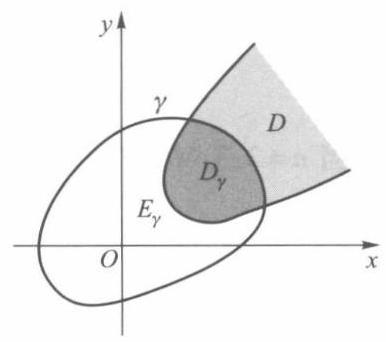
\includegraphics[width=.3\textwidth]{images/P199.jpg}
	\caption{图 $21-43$}
	\label{fig:P199}
\end{figure}

%定理 21.17
\begin{theorem}{}{the:}

\end{theorem}
 设在无界区域 \(D\) 上 \(f\left( {x,y}\right)  \geq  0,{\gamma }_{1}\) , \({\gamma }_{2},\cdots ,{\gamma }_{n},\cdots\) 为一列包围原点的光滑封闭曲线序列,满足

(i) \({d}_{n} = \inf \left\{  {\sqrt{{x}^{2} + {y}^{2}} \mid  \left( {x,y}\right)  \in  {\gamma }_{n}}\right\}   \rightarrow   + \infty \;\left( {n \rightarrow  \infty }\right)\) ,

(ii) \(I = \mathop{\sup }\limits_{n}{\iint }_{{D}_{n}}f\left( {x,y}\right) \mathrm{d}\sigma  <  + \infty\) ,

其中 \({D}_{n}\) 为 \({\gamma }_{n}\) 所围的有界区域 \({E}_{n}\) 与 \(D\) 的交集,则反常二重积分 (1) 收敛, 并且
\[
{\iint }_{D}f\left( {x,y}\right) \mathrm{d}\sigma  = I.
\]
%证
\begin{proof}

\end{proof}
设 \({\gamma }^{\prime }\) 为任何包围原点的光滑封闭曲线,这曲线所围的区域记为 \({E}^{\prime }\) ,并记 \({D}^{\prime } =\)  \({E}^{\prime } \cap  D\) . 因为 \(\mathop{\lim }\limits_{{n \rightarrow  \infty }}{d}_{n} =  + \infty\) ,因此存在 \(n\) ,使得 \({D}^{\prime } \subset  {D}_{n} \subset  D\) . 由于 \(f\left( {x,y}\right)  \geq  0\) ,所以有
\[
{\iint }_{{D}^{\prime }}f\left( {x,y}\right) \mathrm{d}\sigma  \leq  {\iint }_{{D}_{n}}f\left( {x,y}\right) \mathrm{d}\sigma  \leq  I.
\]
另一方面,因为
\[
I = \mathop{\sup }\limits_{n}{\iint }_{{D}_{n}}f\left( {x,y}\right) \mathrm{d}\sigma ,
\]
对于任给的 \(\varepsilon  > 0\) ,总有 \({n}_{0}\) ,使得
\[
{\iint }_{{D}_{{n}_{0}}}f\left( {x,y}\right) \mathrm{d}\sigma  > I - \varepsilon .
\]
对于充分大的 \({d}^{\prime }\) ,区域 \({D}^{\prime }\) 又可包含 \({D}_{{n}_{0}}\) ,因而
\[
{\iint }_{{D}^{\prime }}f\left( {x,y}\right) \mathrm{d}\sigma  > I - \varepsilon .
\]
由
\[
I - \varepsilon  < {\iint }_{{D}^{\prime }}f\left( {x,y}\right) \mathrm{d}\sigma  \leq  I
\]
知 \(f\left( {x,y}\right)\) 在 \(D\) 上的反常二重积分存在,且等于 \(I\) .

由定理 21.17 容易看到: 若在 \(D\) 上 \(f\left( {x,y}\right)  \geq  0\) ,且它在 \(D\) 的任何有界子区域上可积且积分值有界,则 \(f\left( {x,y}\right)\) 在 \(D\) 上的反常二重积分存在. 反过来,若 \(f\left( {x,y}\right)\) 在 \(D\) 上的反常二重积分存在,则 \(f\left( {x,y}\right)\) 在 \(D\) 的任何有界子区域上的积分有上界.

%定理 21.18
\begin{theorem}{}{the:}

\end{theorem}
 若在无界区域 \(D\) 上 \(f\left( {x,y}\right)  \geq  0\) ,则反常二重积分 (1) 收敛的充要条件是: 在 \(D\) 的任何有界子区域上 \(f\left( {x,y}\right)\) 可积,且积分值有上界.

%例 1
\begin{example}

\end{example}
证明反常二重积分
\[
{\iint }_{D}{\mathrm{e}}^{-\left( {{x}^{2} + {y}^{2}}\right) }\mathrm{d}\sigma
\]
收敛,其中 \(D\) 为第一象限部分,即 \(D = \lbrack 0, + \infty ) \times  \lbrack 0, + \infty )\) .

%证
\begin{proof}

\end{proof}
设 \({D}_{R}\) 是以原点为圆心、半径为 \(R\) 的圆与 \(D\) 的交集,即该圆的第一象限部分. 因为 \({\mathrm{e}}^{-\left( {{x}^{2} + {y}^{2}}\right) } > 0\) ,所以二重积分
\[
{\iint }_{{D}_{R}}{\mathrm{e}}^{-\left( {{x}^{2} + {y}^{2}}\right) }\mathrm{d}\sigma
\]
的值随着 \(R\) 的增大而增大. 由于
\[
{\iint }_{{D}_{R}}{\mathrm{e}}^{-\left( {{x}^{2} + {y}^{2}}\right) }\mathrm{d}\sigma  = {\int }_{0}^{\frac{\pi }{2}}\mathrm{\;d}\theta {\int }_{0}^{R}{\mathrm{e}}^{-{r}^{2}}r\mathrm{\;d}r = \frac{\pi }{4}\left( {1 - {\mathrm{e}}^{-{R}^{2}}}\right) ,
\]
所以
\[
\mathop{\lim }\limits_{{R \rightarrow   + \infty }}{\iint }_{{D}_{R}}{\mathrm{e}}^{-\left( {{x}^{2} + {y}^{2}}\right) }\mathrm{d}\sigma  = \mathop{\lim }\limits_{{R \rightarrow   + \infty }}\frac{\pi }{4}\left( {1 - {\mathrm{e}}^{-{R}^{2}}}\right)  = \frac{\pi }{4}.
\]
显然对 \(D\) 的任何有界子区域 \({D}^{\prime }\) ,总存在足够大的 \(R\) ,使得 \({D}^{\prime } \subset  {D}_{R}\) ,于是
\[
{\iint }_{{D}^{\prime }}{\mathrm{e}}^{-\left( {{x}^{2} + {y}^{2}}\right) }\mathrm{d}\sigma  \leq  {\iint }_{{D}_{R}}{\mathrm{e}}^{-\left( {{x}^{2} + {y}^{2}}\right) }\mathrm{d}\sigma  \leq  \frac{\pi }{4}.
\]
因此由定理 21.18 反常二重积分
\[
{\iint }_{D}{\mathrm{e}}^{-\left( {{x}^{2} + {y}^{2}}\right) }\mathrm{d}\sigma
\]
收敛, 并且由定理 21.17 有
\[
{\iint }_{D}{\mathrm{e}}^{-\left( {{x}^{2} + {y}^{2}}\right) }\mathrm{d}\sigma  = \frac{\pi }{4}. \tag{2}
\]
由 (2) 式还可推出在概率论中经常用到的反常积分
\[
{\int }_{0}^{+\infty }{\mathrm{e}}^{-{x}^{2}}\mathrm{\;d}x
\]
的值. 为此,考察 \({S}_{a} = \left\lbrack  {0,a}\right\rbrack   \times  \left\lbrack  {0,a}\right\rbrack\) 上的积分
\[
{\iint }_{{S}_{a}}{\mathrm{e}}^{-\left( {{x}^{2} + {y}^{2}}\right) }\mathrm{d}\sigma
\]
\begin{figure}
	\centering
	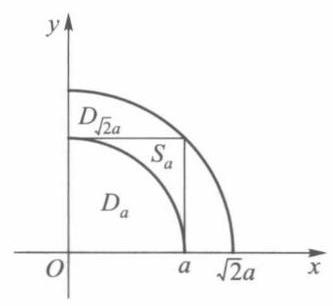
\includegraphics[width=.3\textwidth]{images/P200.jpg}
	\caption{图 $21-44$}
	\label{fig:P200}
\end{figure}

因为
\[
{\iint }_{{S}_{a}}{\mathrm{e}}^{-\left( {{x}^{2} + {y}^{2}}\right) }\mathrm{d}\sigma  = {\int }_{0}^{a}{\mathrm{e}}^{-{x}^{2}}\mathrm{\;d}x{\int }_{0}^{a}{\mathrm{e}}^{-{y}^{2}}\mathrm{\;d}y = {\left( {\int }_{0}^{a}{\mathrm{e}}^{-{x}^{2}}\mathrm{\;d}x\right) }^{2}.
\]
由 \({D}_{a} \subset  {S}_{a} \subset  {D}_{\sqrt{2}a}\) (图 21-44) 知
\[
{\iint }_{{D}_{a}}{\mathrm{e}}^{-\left( {{x}^{2} + {y}^{2}}\right) }\mathrm{d}\sigma  \leq  {\iint }_{{S}_{a}}{\mathrm{e}}^{-\left( {{x}^{2} + {y}^{2}}\right) }\mathrm{d}\sigma
\]

\[
= {\left( {\int }_{0}^{a}{\mathrm{e}}^{-{x}^{2}}\mathrm{\;d}x\right) }^{2} \leq  {\iint }_{{D}_{\sqrt{2}a}}{\mathrm{e}}^{-\left( {{x}^{2} + {y}^{2}}\right) }\mathrm{d}\sigma .
\]
令 \(a \rightarrow   + \infty\) ,则得
\[
\mathop{\lim }\limits_{{a \rightarrow   + \infty }}{\left( {\int }_{0}^{a}{\mathrm{e}}^{-{x}^{2}}\mathrm{\;d}x\right) }^{2} = {\iint }_{D}{\mathrm{e}}^{-\left( {{x}^{2} + {y}^{2}}\right) }\mathrm{d}\sigma  = \frac{\pi }{4}.
\]
所以
\[
{\int }_{0}^{+\infty }{\mathrm{e}}^{-{x}^{2}}\mathrm{\;d}x = \frac{\sqrt{\pi }}{2}.
\]
下面的例子是应用反常二重积分补证第十九章最后提到的关于 \(\mathrm{B}\) 函数与 \(\Gamma\) 函数的联系公式. 例 2 若 \(p > 0,q > 0\) ,则
\[
\mathrm{B}\left( {p,q}\right)  = \frac{\Gamma \left( p\right) \Gamma \left( q\right) }{\Gamma \left( {p + q}\right) }. \tag{3}
\]
%证
\begin{proof}

\end{proof}
对于 \(\Gamma\) 函数,令 \(x = {u}^{2}\) ,则 \(\mathrm{d}x = {2u}\mathrm{\;d}u\) ,于是
\[
\Gamma \left( p\right)  = {\int }_{0}^{+\infty }{x}^{p - 1}{\mathrm{e}}^{-x}\mathrm{\;d}x = 2{\int }_{0}^{+\infty }{u}^{{2p} - 1}{\mathrm{e}}^{-{u}^{2}}\mathrm{\;d}u.
\]
从而
\[
\Gamma \left( p\right) \Gamma \left( q\right)  = 4{\int }_{0}^{+\infty }{x}^{{2p} - 1}{\mathrm{e}}^{-{x}^{2}}\mathrm{\;d}x \cdot  {\int }_{0}^{+\infty }{y}^{{2q} - 1}{\mathrm{e}}^{-{y}^{2}}\mathrm{\;d}y
\]
\[
= \mathop{\lim }\limits_{{R \rightarrow   + \infty }}4{\int }_{0}^{R}{x}^{{2p} - 1}{\mathrm{e}}^{-{x}^{2}}\mathrm{\;d}x \cdot  {\int }_{0}^{R}{y}^{{2q} - 1}{\mathrm{e}}^{-{y}^{2}}\mathrm{\;d}y.
\]
令 \({D}_{R} = \left\lbrack  {0,R}\right\rbrack   \times  \left\lbrack  {0,R}\right\rbrack\) ,由二重积分化为累次积分计算公式有
\[
{\iint }_{{D}_{R}}{x}^{{2p} - 1}{y}^{{2q} - 1}{\mathrm{e}}^{-\left( {{x}^{2} + {y}^{2}}\right) }\mathrm{d}\sigma
\]
\[
= {\int }_{0}^{R}{x}^{{2p} - 1}{\mathrm{e}}^{-{x}^{2}}\mathrm{\;d}x \cdot  {\int }_{0}^{R}{y}^{{2q} - 1}{\mathrm{e}}^{-{y}^{2}}\mathrm{\;d}y.
\]
所以
\[
\Gamma \left( p\right) \Gamma \left( q\right)  = \mathop{\lim }\limits_{{R \rightarrow   + \infty }}4{\iint }_{{D}_{R}}{x}^{{2p} - 1}{y}^{{2q} - 1}{\mathrm{e}}^{-\left( {{x}^{2} + {y}^{2}}\right) }\mathrm{d}\sigma
\]
\[
= 4{\iint }_{D}{x}^{{2p} - 1}{y}^{{2q} - 1}{\mathrm{e}}^{-\left( {{x}^{2} + {y}^{2}}\right) }\mathrm{d}\sigma , \tag{4}
\]
这里 \(D\) 为平面上第一象限部分. 和例 1 一样,下面讨论 (4) 式右边的反常二重积分. 记
\[
{D}_{r} = \left\{  {\left( {x,y}\right)  \mid  {x}^{2} + {y}^{2} \leq  {r}^{2},x \geq  0,y \geq  0}\right\}  .
\]
于是有
\[
\Gamma \left( p\right) \Gamma \left( q\right)  = 4{\iint }_{D}{x}^{{2p} - 1}{y}^{{2q} - 1}{\mathrm{e}}^{-\left( {{x}^{2} + {y}^{2}}\right) }\mathrm{d}\sigma
\]
\[
= \mathop{\lim }\limits_{{r \rightarrow   + \infty }}4{\iint }_{{D}_{r}}{x}^{{2p} - 1}{y}^{{2q} - 1}{\mathrm{e}}^{-\left( {{x}^{2} + {y}^{2}}\right) }\mathrm{d}\sigma .
\]
对上式右边积分应用极坐标变换, 则可得
\[
\Gamma \left( p\right) \Gamma \left( q\right)  = \mathop{\lim }\limits_{{r \rightarrow   + \infty }}4{\int }_{0}^{\frac{\pi }{2}}\mathrm{\;d}\theta {\int }_{0}^{r}{r}^{2\left( {p + q}\right)  - 2}{\left( \cos \theta \right) }^{{2p} - 1}{\left( \sin \theta \right) }^{{2q} - 1}{\mathrm{e}}^{-{r}^{2}}r\mathrm{\;d}r
\]
\[
= \mathop{\lim }\limits_{{r \rightarrow   + \infty }}2{\int }_{0}^{\frac{\pi }{2}}{\left( \cos \theta \right) }^{{2p} - 1}{\left( \sin \theta \right) }^{{2q} - 1}\mathrm{\;d}\theta  \cdot  2{\int }_{0}^{r}{r}^{2\left( {p + q}\right)  - 1}{\mathrm{e}}^{-{r}^{2}}\mathrm{\;d}r
\]
\[
= 2{\int }_{0}^{\frac{\pi }{2}}{\left( \cos \theta \right) }^{{2p} - 1}{\left( \sin \theta \right) }^{{2q} - 1}\mathrm{\;d}\theta  \cdot  \Gamma \left( {p + q}\right) .
\]
再由第十九章 §3 的(11)式就得到
\[
\Gamma \left( p\right) \Gamma \left( q\right)  = \mathrm{B}\left( {p,q}\right) \Gamma \left( {p + q}\right) .
\]
%定理 21.19
\begin{theorem}{}{the:}

\end{theorem}
 函数 \(f\left( {x,y}\right)\) 在无界区域 \(D\) 上的反常二重积分收敛的充要条件是 \(\left| {f\left( {x,y}\right) }\right|\) 在 \(D\) 上的反常二重积分收敛.

%证
\begin{proof}

\end{proof}
我们先证充分性. 设 \({\iint }_{D}\left| {f\left( {x,y}\right) }\right| \mathrm{d}\sigma\) 收敛,其值为 \(M\) . 作辅助函数
\[
{f}^{ + }\left( {x,y}\right)  = \frac{\left| {f\left( {x,y}\right) }\right|  + f\left( {x,y}\right) }{2},{f}^{ - }\left( {x,y}\right)  = \frac{\left| {f\left( {x,y}\right) }\right|  - f\left( {x,y}\right) }{2}.
\]
显然有 \(0 \leq  {f}^{ + }\left( {x,y}\right)  \leq  \left| {f\left( {x,y}\right) }\right|\) 及 \(0 \leq  {f}^{ - }\left( {x,y}\right)  \leq  \left| {f\left( {x,y}\right) }\right|\) . 因而在 \(D\) 的任何有界子区域 \(\sigma\) 上,恒有
\[
{\iint }_{\sigma }{f}^{ + }\left( {x,y}\right) \mathrm{d}\sigma  \leq  {\iint }_{\sigma }\left| {f\left( {x,y}\right) }\right| \mathrm{d}\sigma  = M,
\]
\[
{\iint }_{\sigma }{f}^{ - }\left( {x,y}\right) \mathrm{d}\sigma  \leq  {\iint }_{\sigma }\left| {f\left( {x,y}\right) }\right| \mathrm{d}\sigma  = M.
\]
所以 \({f}^{ + }\left( {x,y}\right)\) 与 \({f}^{ - }\left( {x,y}\right)\) 在 \(D\) 上的反常二重积分收敛. 由于
\[
f\left( {x,y}\right)  = {f}^{ + }\left( {x,y}\right)  - {f}^{ - }\left( {x,y}\right) ,
\]
所以 \(f\left( {x,y}\right)\) 在 \(D\) 上的反常二重积分也收敛.

关于必要性的证明, 这里不讲了. 有兴趣的读者可参阅菲赫金哥尔茨著的微积分学教程第三卷第一分册.

%定理 21.20
\begin{theorem}{}{the:}

\end{theorem}
 (柯西判别法) 设 \(f\left( {x,y}\right)\) 在无界区域 \(D\) 的任何有界子区域上二重积分存在, \(r\) 为 \(D\) 内的点(x, y)到原点的距离
\[
r = \sqrt{{x}^{2} + {y}^{2}}.
\]
(i) 若当 \(r\) 足够大时, \(\left| {f\left( {x,y}\right) }\right|  \leq  \frac{c}{{r}^{p}}\) ,其中 \(c\) 为正的常数,则当 \(p > 2\) 时,反常二重积分 \({\iint }_{D}f\left( {x,y}\right) \mathrm{d}\sigma\) 收敛;

(ii) 若 \(f\left( {x,y}\right)\) 在 \(D\) 内满足 \(\left| {f\left( {x,y}\right) }\right|  \geq  \frac{c}{{r}^{p}}\) ,其中 \(D\) 是含有顶点为原点的无限扇形区域,则当 \(p \leq  2\) 时,反常二重积分 \({\iint }_{D}f\left( {x,y}\right) \mathrm{d}\sigma\) 发散.

证明从略.

\subsection{无界函数的二重积分}

%定义  2
\begin{definition}{}{def:}

\end{definition}
设 \(P\) 为有界区域 \(D\) 的一个聚点, \(f\left( {x,y}\right)\) 在 \(D\) 上除点 \(P\) 外皆有定义,且在 \(P\) 的任何空心邻域内无界, \(\Delta\) 为 \(D\) 中任何含有 \(P\) 的小区域, \(f\left( {x,y}\right)\) 在 \(D - \Delta\) 上可积. 又设 \(d\) 表示 \(\Delta\) 的直径,即
\[
d = \sup \left\{  {\sqrt{{\left( {x}_{1} - {x}_{2}\right) }^{2} + {\left( {y}_{1} - {y}_{2}\right) }^{2}} \mid  \left( {{x}_{1},{y}_{1}}\right) ,\left( {{x}_{2},{y}_{2}}\right)  \in  \Delta }\right\}  .
\]
若极限
\[
\mathop{\lim }\limits_{{d \rightarrow  0}}{\iint }_{D - \Delta }f\left( {x,y}\right) \mathrm{d}\sigma
\]
存在且有限,并且与 \(\Delta\) 的取法无关,则称 \(f\left( {x,y}\right)\) 在 \(D\) 上的反常二重积分收敛,记作
\[
{\iint }_{D}f\left( {x,y}\right) \mathrm{d}\sigma  = \mathop{\lim }\limits_{{d \rightarrow  0}}{\iint }_{D - \Delta }f\left( {x,y}\right) \mathrm{d}\sigma ,
\]
否则称 \(f\left( {x,y}\right)\) 在 \(D\) 上的反常二重积分 \({\iint }_{D}f\left( {x,y}\right) \mathrm{d}\sigma\) 发散.

与无界区域上反常二重积分一样, 对无界函数的反常二重积分也可建立相应的收敛性定理.

%定理 21.21
\begin{theorem}{}{the:}

\end{theorem}
 (柯西判别法) 设 \(f\left( {x,y}\right)\) 在有界区域 \(D\) 上除点 \(P\left( {{x}_{0},{y}_{0}}\right)\) 外处处有定义,点 \(P\left( {{x}_{0},{y}_{0}}\right)\) 为它的瑕点,则下面两个结论成立:

(i) 若在点 \(P\) 的附近有
\[
\left| {f\left( {x,y}\right) }\right|  \leq  \frac{c}{{r}^{\alpha }},
\]
其中 \(c\) 为常数, \(r = \sqrt{{\left( x - {x}_{0}\right) }^{2} + {\left( y - {y}_{0}\right) }^{2}}\) ,则当 \(\alpha  < 2\) 时,反常二重积分 \({\iint }_{D}f\left( {x,y}\right) \mathrm{d}\sigma\) 收敛;

(ii) 若在点 \(P\) 的附近有
\[
\left| {f\left( {x,y}\right) }\right|  \geq  \frac{c}{{r}^{\alpha }},
\]
且 \(D\) 含有以点 \(P\) 为顶点的角形区域,则当 \(\alpha  \geq  2\) 时,反常二重积分 \({\iint }_{D}f\left( {x,y}\right) \mathrm{d}\sigma\) 发散.

\subsection{习题 21.8}

1. 试讨论下列无界区域上二重积分的收敛性:

(1) \({\iint }_{{x}^{2} + {y}^{2} \geq  1}\frac{\mathrm{d}\sigma }{{\left( {x}^{2} + {y}^{2}\right) }^{m}}\) ;

(2) \({\iint }_{D}\frac{\mathrm{d}\sigma }{{\left( 1 + \left| x\right| \right) }^{p}{\left( 1 + \left| y\right| \right) }^{q}},D\) 为全平面；

(3) \({\iint }_{0 \leq  y \leq  1}\frac{\varphi \left( {x,y}\right) \mathrm{d}\sigma }{{\left( 1 + {x}^{2} + {y}^{2}\right) }^{p}}\;\left( {0 < m \leq  \left| {\varphi \left( {x,y}\right) }\right|  \leq  M}\right)\) .

2. 计算积分
\[
{\int }_{-\infty }^{+\infty }\mathrm{d}y{\int }_{-\infty }^{+\infty }{\mathrm{e}}^{-\left( {{x}^{2} + {y}^{2}}\right) }\cos \left( {{x}^{2} + {y}^{2}}\right) \mathrm{d}x.
\]
3. 判别下列积分的敛散性:

(1) \({\iint }_{{x}^{2} + {y}^{2} \leq  1}\frac{\mathrm{d}\sigma }{{\left( {x}^{2} + {y}^{2}\right) }^{m}};\;\left( 2\right) {\iint }_{{x}^{2} + {y}^{2} \leq  1}\frac{\mathrm{d}\sigma }{{\left( 1 - {x}^{2} - {y}^{2}\right) }^{m}}\) .

\section{在一般条件下重积分变量变换公式的证明}

我们在本章 §4 中证明了重积分变量变换公式(定理 21.13). 在证明中引用了 §4 中的引理. 此引理需要较强条件: \(x\left( {u,v}\right) ,y\left( {u,v}\right)\) 有二阶连续偏导数. 本节将在 \(x\left( {u,v}\right)\) , \(y\left( {u,v}\right)\) 仅有一阶连续偏导数的条件下来证明 §4 中的引理,这样我们就完成了在一般条件下二重积分的变量变换公式. 为此, 我们把这个引理重新叙述如下.

引理 设变换 \(T : x = x\left( {u,v}\right) ,y = y\left( {u,v}\right)\) 把 \({uv}\) 平面上的由分段光滑封闭曲线所围的闭区域 \(\Delta\) 一对一地映成 \({xy}\) 平面上的闭区域 \(D\) ,函数 \(x = x\left( {u,v}\right) ,y = y\left( {u,v}\right)\) 在 \(\Delta\) 上分别具有一阶连续偏导数且它们的函数行列式
\[
J\left( {u,v}\right)  = \frac{\partial \left( {x,y}\right) }{\partial \left( {u,v}\right) } \neq  0,\left( {u,v}\right)  \in  \Delta ,
\]
则区域 \(D\) 的面积
\[
\mu \left( D\right)  = {\iint }_{\Delta }\left| {J\left( {u,v}\right) }\right| \mathrm{d}u\mathrm{\;d}v.
\]
%证
\begin{proof}

\end{proof}
证明分以下 4 步:

第 1 步: 对任意 \(\left( {{u}_{0},{v}_{0}}\right)  \in  \operatorname{int}\Delta\) ,任意 \(\varepsilon  > 0\) ,存在 \(\left( {{u}_{0},{v}_{0}}\right)\) 的邻域 \(G\) ,当正方形 \(I \subset  G\) 且 \(\left( {{u}_{0},{v}_{0}}\right)  \in  I\) 时,
\[
\mu \left( {T\left( I\right) }\right)  \leq  {\iint }_{I}\left| {J\left( {u,v}\right) }\right| \mathrm{d}u\mathrm{\;d}v + {\varepsilon \mu }\left( I\right) .
\]
第 2 步: 对任意正方形 \(I \subset  \operatorname{int}\Delta ,\mu \left( {T\left( I\right) }\right)  \leq  {\iint }_{I}\left| {J\left( {u,v}\right) }\right| \mathrm{d}u\mathrm{\;d}v\) .

第 3 步: \(\mu \left( D\right)  \leq  {\iint }_{\Delta }\left| {J\left( {u,v}\right) }\right| \mathrm{d}u\mathrm{\;d}v\) .

第 4 步: \(\mu \left( D\right)  = {\iint }_{\Delta }\left| {J\left( {u,v}\right) }\right| \mathrm{d}u\mathrm{\;d}v\) .

第 1 步的证明 设 \(\left( {{u}_{0},{v}_{0}}\right)  \in  \operatorname{int}\Delta\) ,对任意 \(\varepsilon  > 0\) ,取正数 \(\eta  < \left| {J\left( {{u}_{0},{v}_{0}}\right) }\right|\) 满足
\[
{\left( 1 + \eta \right) }^{2}\left| {J\left( {{u}_{0},{v}_{0}}\right) }\right|  < \left| {J\left( {{u}_{0},{v}_{0}}\right) }\right|  - \eta  + \varepsilon .
\]
由于 \(\left| {J\left( {u,v}\right) }\right|\) 在点 \(\left( {{u}_{0},{v}_{0}}\right)\) 上连续,因此存在 \(\left( {{u}_{0},{v}_{0}}\right)\) 的邻域 \({G}_{1} \subset  \operatorname{int}\Delta\) ,使得当(u, v) \(\in  {G}_{1}\) 时,
\[
\left| {J\left( {u,v}\right) }\right|  > \left| {J\left( {{u}_{0},{v}_{0}}\right) }\right|  - \eta .
\]
定义映射
\[
L : \left\{  \begin{array}{l} \widehat{x}\left( {u,v}\right)  = x\left( {{u}_{0},{v}_{0}}\right)  + {x}_{u}\left( {{x}_{0},{v}_{0}}\right) \left( {u - {u}_{0}}\right)  + {x}_{v}\left( {{u}_{0},{v}_{0}}\right) \left( {v - {v}_{0}}\right) , \\  \widehat{y}\left( {u,v}\right)  = y\left( {{u}_{0},{v}_{0}}\right)  + {y}_{u}\left( {{u}_{0},{v}_{0}}\right) \left( {u - {u}_{0}}\right)  + {y}_{v}\left( {{u}_{0},{v}_{0}}\right) \left( {v - {v}_{0}}\right) , \end{array}\right.
\]
即
\[
L\left( {u,v}\right)  = \left( \begin{array}{l} \widehat{x}\left( {u,v}\right) \\  \widehat{y}\left( {u,v}\right)  \end{array}\right)  = \left( \begin{array}{l} x\left( {{u}_{0},{v}_{0}}\right) \\  y\left( {{u}_{0},{v}_{0}}\right)  \end{array}\right)  + {\mathbf{J}}_{T}\left( {{u}_{0},{v}_{0}}\right) \left( \begin{array}{l} u - {u}_{0} \\  v - {v}_{0} \end{array}\right) ,
\]
其中 \({\mathbf{J}}_{T}\left( {{u}_{0},{v}_{0}}\right)  = \left( \begin{array}{ll} {x}_{u}\left( {{u}_{0},{v}_{0}}\right) & {x}_{v}\left( {{u}_{0},{v}_{0}}\right) \\  {y}_{u}\left( {{u}_{0},{v}_{0}}\right) & {y}_{v}\left( {{u}_{0},{v}_{0}}\right)  \end{array}\right)\) .

由于 \(x\left( {u,v}\right) ,y\left( {u,v}\right)\) 在 \(\left( {{u}_{0},{v}_{0}}\right)\) 处可微,因此
\[
\left| {x\left( {u,v}\right)  - \widehat{x}\left( {u,v}\right) }\right|
\]
\[
= \left| {x\left( {u,v}\right)  - x\left( {{u}_{0},{v}_{0}}\right)  - {x}_{u}\left( {{u}_{0},{v}_{0}}\right) \left( {u - {u}_{0}}\right)  - {x}_{v}\left( {{u}_{0},{v}_{0}}\right) \left( {v - {v}_{0}}\right) }\right|
\]
\[
= o\left( \rho \right) \left( {\rho  \rightarrow  0}\right) \text{ , }
\]
\[
\left| {y\left( {u,v}\right)  - \widehat{y}\left( {u,v}\right) }\right|
\]
\[
= \left| {y\left( {u,v}\right)  - y\left( {{u}_{0},{v}_{0}}\right)  - {y}_{u}\left( {{u}_{0},{v}_{0}}\right) \left( {u - {u}_{0}}\right)  - {y}_{v}\left( {{u}_{0},{v}_{0}}\right) \left( {v - {v}_{0}}\right) }\right|
\]
\[
= o\left( \rho \right) \left( {\rho  \rightarrow  0}\right) \text{ , }
\]
其中
\[
\rho  = \sqrt{{\left( u - {u}_{0}\right) }^{2} + {\left( v - {v}_{0}\right) }^{2}}.
\]
设 \({\left( {\mathbf{J}}_{T}\left( {u}_{0},{v}_{0}\right) \right) }^{-1} = \left( \begin{array}{ll} a & b \\  c & d \end{array}\right)\) ,令 \(M = \left| a\right|  + \left| b\right|  + \left| c\right|  + \left| d\right|\) . 存在 \(\left( {{u}_{0},{v}_{0}}\right)\) 的邻域 \(G \subset  {G}_{1}\) ,当 \(\left( {u,v}\right)  \in  G\) 时,
\[
\left| {x\left( {u,v}\right)  - \widehat{x}\left( {u,v}\right) }\right|  < \frac{\eta \rho }{2\sqrt{2}M},\left| {y\left( {u,v}\right)  - \widehat{y}\left( {u,v}\right) }\right|  < \frac{\eta \rho }{2\sqrt{2}M}.
\]
任取正方形 \(I \subset  \operatorname{int}\Delta\) ,满足 \(\left( {{u}_{0},{v}_{0}}\right)  \in  I\) ,并设 \(I\) 的边长为 \(\beta\) . 任取 \(\left( {x\left( {u,v}\right) ,y\left( {u,v}\right) }\right)  \in\)  \(T\left( I\right)\) ,其中 \(\left( {u,v}\right)  \in  I\) .

设 \(\left( {{u}_{1},{v}_{1}}\right)  = {L}^{-1}\left( {x\left( {u,v}\right) ,y\left( {u,v}\right) }\right)\) ,即 \(\widehat{x}\left( {{u}_{1},{v}_{1}}\right)  = x\left( {u,v}\right) ,\widehat{y}\left( {{u}_{1},{v}_{1}}\right)  = y\left( {u,v}\right)\) . 由于
\[
\left( \begin{array}{l} \widehat{x}\left( {{u}_{1},{v}_{1}}\right)  - \widehat{x}\left( {u,v}\right) \\  \widehat{y}\left( {{u}_{1},{v}_{1}}\right)  - \widehat{y}\left( {u,v}\right)  \end{array}\right)  = {\mathbf{J}}_{T}\left( {{u}_{0},{v}_{0}}\right) \left( \begin{array}{l} {u}_{1} - u \\  {v}_{1} - v \end{array}\right) ,
\]
因此
\[
\left( \begin{array}{l} {u}_{1} - u \\  {v}_{1} - v \end{array}\right)  = {\left( {\mathbf{J}}_{T}\left( {u}_{0},{v}_{0}\right) \right) }^{-1}\left( \begin{array}{l} \widehat{x}\left( {{u}_{1},{v}_{1}}\right)  - \widehat{x}\left( {u,v}\right) \\  \widehat{y}\left( {{u}_{1},{v}_{1}}\right)  - \widehat{y}\left( {u,v}\right)  \end{array}\right)  = \left( \begin{array}{ll} a & b \\  c & d \end{array}\right) \left( \begin{array}{l} \widehat{x}\left( {{u}_{1},{v}_{1}}\right)  - \widehat{x}\left( {u,v}\right) \\  \widehat{y}\left( {{u}_{1},{v}_{1}}\right)  - \widehat{y}\left( {u,v}\right)  \end{array}\right) .
\]
注意到 \(\rho  = \sqrt{{\left( u - {u}_{0}\right) }^{2} + {\left( v - {v}_{0}\right) }^{2}},\left( {u,v}\right)  \in  I,\left( {{u}_{0},{v}_{0}}\right)  \in  I\) ,从而 \(\rho  \leq  \sqrt{2}\beta\) ,于是
\[
\left| {{u}_{1} - u}\right|  = \left| {a\left( {\widehat{x}\left( {{u}_{1},{v}_{1}}\right)  - \widehat{x}\left( {u,v}\right) }\right)  + b\left( {\widehat{y}\left( {{u}_{1},{v}_{1}}\right)  - \widehat{y}\left( {u,v}\right) }\right) }\right|
\]
\[
= \left| {a\left( {x\left( {u,v}\right)  - \widehat{x}\left( {u,v}\right) }\right)  + b\left( {y\left( {u,v}\right)  - \widehat{y}\left( {u,v}\right) }\right) }\right|
\]
\[
< \left| a\right| \left| {x\left( {u,v}\right)  - \widehat{x}\left( {u,v}\right) }\right|  + \left| b\right| \left| {y\left( {u,v}\right)  - \widehat{y}\left( {u,v}\right) }\right|
\]
\[
\leq  \left| a\right| \frac{\eta \rho }{2\sqrt{2}M} + \left| b\right| \frac{\eta \rho }{2\sqrt{2}M} \leq  \left| a\right| \frac{\eta \beta }{2M} + \left| b\right| \frac{\eta \beta }{2M} \leq  \frac{\eta \beta }{2}.
\]
同理 \(\left| {{v}_{1} - v}\right|  \leq  \frac{\eta \beta }{2}\) .

设 \({I}_{1}\) 是与 \(I\) 同中心的正方形,边长为 \(\left( {1 + \eta }\right) \beta\) ,从而 \(\left( {{u}_{1},{v}_{1}}\right)  \in  {I}_{1}\) . 于是
\[
T\left( {u,v}\right)  = \left( {x\left( {u,v}\right) ,y\left( {u,v}\right) }\right)  = L\left( {{u}_{1},{v}_{1}}\right)  \in  L\left( {I}_{1}\right) ,
\]
这样就证明了 \(T\left( I\right)  \subset  L\left( {I}_{1}\right)\) .

设 \({I}_{1}\) 的二邻边向量是 \({l}_{1},{l}_{2}\) ,由于 \(L\) 是仿射变换, \(L\left( {I}_{1}\right)\) 是邻边向量为 \(L\left( {l}_{1}\right) ,L\left( {l}_{2}\right)\) 的平行四边形, 于是
\[
\mu \left( {L\left( {I}_{1}\right) }\right)  = \left| {L\left( {\mathbf{l}}_{1}\right)  \times  L\left( {\mathbf{l}}_{2}\right) }\right|  = \left| {J\left( {{u}_{0},{v}_{0}}\right) }\right| \left| {{\mathbf{l}}_{1} \times  {\mathbf{l}}_{2}}\right|  = \left| {J\left( {{u}_{0},{v}_{0}}\right) }\right| \mu \left( {I}_{1}\right) .
\]
因此
\[
\mu \left( {T\left( I\right) }\right)  \leq  \mu \left( {L\left( {I}_{1}\right) }\right)  = \left| {J\left( {{u}_{0},{v}_{0}}\right) }\right| \mu \left( {I}_{1}\right)  = \left| {J\left( {{u}_{0},{v}_{0}}\right) }\right| {\left( 1 + \eta \right) }^{2}\mu \left( I\right) .
\]
另一方面,我们有
\[
{\iint }_{I}\left| {J\left( {u,v}\right) }\right| \mathrm{d}u\mathrm{\;d}v \geq  \left( {\left| {J\left( {{u}_{0},{v}_{0}}\right) }\right|  - \eta }\right) \mu \left( I\right) ,
\]
因此
\[
\mu \left( {T\left( I\right) }\right)  \leq  \left| {J\left( {{u}_{0},{v}_{0}}\right) }\right| {\left( 1 + \eta \right) }^{2}\mu \left( I\right)
\]
\[
\leq  \left( {\left| {J\left( {{u}_{0},{v}_{0}}\right) }\right|  - \eta  + \varepsilon }\right) \mu \left( I\right)
\]
\[
\leq  {\iint }_{I}\left| {J\left( {u,v}\right) }\right| \mathrm{d}u\mathrm{\;d}v + {\varepsilon \mu }\left( I\right) .
\]
第 2 步的证明 若有正方形 \(I \subset  \operatorname{int}\Delta\) ,使
\[
\mu \left( {T\left( I\right) }\right)  - {\iint }_{I}\left| {J\left( {u,v}\right) }\right| \mathrm{d}u\mathrm{\;d}v = \delta  > 0,
\]
将 \(I\) 等分为 4 个小正方形,则 4 个正方形中必有一个,记为 \({I}_{1}\) ,使
\[
\mu \left( {T\left( {I}_{1}\right) }\right)  - {\iint }_{{I}_{1}}\left| {J\left( {u,v}\right) }\right| \mathrm{d}u\mathrm{\;d}v \geq  \frac{\delta }{4}.
\]
再将 \({I}_{1}\) 等分为 4 个小正方形,则 4 个正方形中必有一个,记为 \({I}_{2}\) ,使
\[
\mu \left( {T\left( {I}_{2}\right) }\right)  - {\iint }_{{I}_{2}}\left| {J\left( {u,v}\right) }\right| \mathrm{d}u\mathrm{\;d}v \geq  \frac{\delta }{{4}^{2}}.
\]
这样我们得到正方形序列 \({I}_{1} \supset  {I}_{2} \supset  \cdots  \supset  {I}_{n} \supset  \cdots\) ,使
\[
\mu \left( {T\left( {I}_{n}\right) }\right)  - {\iint }_{{I}_{n}}\left| {J\left( {u,v}\right) }\right| \mathrm{d}u\mathrm{\;d}v \geq  \frac{\delta }{{4}^{n}}.
\]
由闭域套定理 (定理 16.2),存在 \(\left( {{u}_{0},{v}_{0}}\right)  \in  \mathop{\bigcap }\limits_{{n = 1}}^{\infty }{I}_{n} \subset  \operatorname{int}\Delta\) . 于是任给 \(\varepsilon  > 0\) ,存在 \(\left( {{u}_{0},{v}_{0}}\right)\) 的开邻域 \(G \subset  \operatorname{int}\Delta\) 满足第 1 步的结论,于是当 \(n\) 充分大时 \({I}_{n} \subset  G\) ,从而
\[
\frac{{\varepsilon \mu }\left( I\right) }{{4}^{n}} = {\varepsilon \mu }\left( {I}_{n}\right)  \geq  \mu \left( {T\left( {I}_{n}\right) }\right)  - {\iint }_{{I}_{n}}\left| {J\left( {u,v}\right) }\right| \mathrm{d}u\mathrm{\;d}v \geq  \frac{\delta }{{4}^{n}},
\]
即 \({\varepsilon \mu }\left( I\right)  \geq  \delta  > 0\) ,令 \(\varepsilon  \rightarrow  0\) 得到 \(0 \geq  \delta  > 0\) ,矛盾.

第 3 步的证明 用平行于坐标轴的直线将 \({uv}\) 平面分割成大小相等的闭正方形,假定与 int \(\Delta\) 交集不空的正方形为 \(\left\{  {{I}_{1},{I}_{2},\cdots ,{I}_{n}}\right\}\) ,其中完全在 int \(\Delta\) 内正方形为 \(\left\{  {I}_{1}^{\prime }\right.\) , \(\left. {{I}_{2}^{\prime },\cdots ,{I}_{s}^{\prime }}\right\}\) ,不完全在 int \(\Delta\) 内的正方形为 \(\left\{  {{I}_{1}^{\prime \prime },{I}_{2}^{\prime \prime },\cdots ,{I}_{t}^{\prime \prime }}\right\}\) . 作 \(\Delta\) 的分割 \({T}_{\Delta } = \left\{  {{I}_{i} \cap  \Delta  \mid  i = 1}\right.\) , \(2,\cdots ,n\}\) 和 \(D\) 的分割 \({T}_{D} = \left\{  {T\left( {{I}_{i} \cap  \Delta }\right)  \mid  i = 1,2,\cdots ,n}\right\}\) . 由于 \(T\) 在 \(\Delta\) 上的一致连续性,当 \(\begin{Vmatrix}{T}_{\Delta }\end{Vmatrix} \rightarrow  0\) 时, \(\begin{Vmatrix}{T}_{D}\end{Vmatrix} \rightarrow  0\) . 又因为 \(\partial \Delta  \subset  \mathop{\bigcup }\limits_{{i = 1}}^{t}\left( {{I}_{i}^{\prime \prime } \cap  \Delta }\right)\) 及 \(\partial D \subset  \mathop{\bigcup }\limits_{{i = 1}}^{t}T\left( {{I}_{i}^{\prime \prime } \cap  \Delta }\right)\) ,我们可证
\[
\mathop{\lim }\limits_{{\begin{Vmatrix}{T}_{\Delta }\end{Vmatrix} \rightarrow  0}}\mathop{\sum }\limits_{{i = 1}}^{t}\mu \left( {{I}_{i}^{\prime \prime } \cap  \Delta }\right)  = 0\;\text{ 和 }\;\mathop{\lim }\limits_{{\begin{Vmatrix}{T}_{D}\end{Vmatrix} \rightarrow  0}}\mathop{\sum }\limits_{{i = 1}}^{t}\mu \left( {T\left( {{I}_{i}^{\prime \prime } \cap  \Delta }\right) }\right)  = 0
\]
同时成立. 为此,定义 \(\Delta\) 上的函数 \(\varphi \left( {u,v}\right)  = \left\{  \begin{array}{l} 1,\left( {u,v}\right)  \in  \operatorname{int}\Delta \\  0,\left( {u,v}\right)  \in  \partial \Delta . \end{array}\right.\)

由于 \(\varphi \left( {u,v}\right)\) 仅在零面积集 \(\partial \Delta\) 上不连续,因此由定理 21.7, \(\varphi \left( {u,v}\right)\) 在 \(\Delta\) 上可积. 又由定理 21.4, \(\mathop{\lim }\limits_{{\begin{Vmatrix}{T}_{\Delta }\end{Vmatrix} \rightarrow  0}}\mathop{\sum }\limits_{{i = 1}}^{n}{\omega }_{i}\mu \left( {{I}_{i} \cap  \Delta }\right)  = 0\) ,其中 \({\omega }_{i}\) 是 \(\varphi \left( {u,v}\right)\) 在 \({I}_{i} \cap  \Delta\) 上的振幅. 因为 \({I}_{i}^{\prime \prime }\) 不完全在 int \(\Delta\) 内,且至少有一个内点, \({\omega }^{\prime \prime }{}_{i} = 1\) . 而 \({I}_{i}^{\prime }\) 完全在 int \(\Delta\) 内, \({\omega }_{i}^{\prime } = 0\) . 所以
\[
\mathop{\lim }\limits_{{\begin{Vmatrix}{T}_{\Delta }\end{Vmatrix} \rightarrow  0}}\mathop{\sum }\limits_{{i = 1}}^{t}\mu \left( {{I}_{i}^{\prime \prime } \cap  \Delta }\right)  = \mathop{\lim }\limits_{{\begin{Vmatrix}{T}_{\Delta }\end{Vmatrix} \rightarrow  0}}\mathop{\sum }\limits_{{i = 1}}^{n}{\omega }_{i}\mu \left( {{I}_{i} \cap  \Delta }\right)  = 0.
\]
类似可证 \(\mathop{\lim }\limits_{{\begin{Vmatrix}{T}_{D}\end{Vmatrix} \rightarrow  0}}\mathop{\sum }\limits_{{i = 1}}^{t}\mu \left( {T\left( {{I}_{i}^{\prime \prime } \cap  \Delta }\right) }\right)  = 0\) .

设 \(\left| {J\left( {u,v}\right) }\right|\) 在 \(\Delta\) 上的上确界为 \(M\) ,则
\[
0 \leq  {\iint }_{\Delta }\left| {J\left( {u,v}\right) }\right| \mathrm{d}u\mathrm{\;d}v - \mathop{\sum }\limits_{{i = 1}}^{s}{\iint }_{{I}_{i}^{\prime }}\left| {J\left( {u,v}\right) }\right| \mathrm{d}u\mathrm{\;d}v
\]
\[
= \mathop{\sum }\limits_{{i = 1}}^{t}{\iint }_{{I}_{i}^{n} \cap  \Delta }\left| {J\left( {u,v}\right) }\right| \mathrm{d}u\mathrm{\;d}v \leq  M\mathop{\sum }\limits_{{i = 1}}^{t}\mu \left( {{I}_{i}^{\prime \prime } \cap  \Delta }\right)  \rightarrow  0\left( {\begin{Vmatrix}{T}_{\Delta }\end{Vmatrix} \rightarrow  0}\right) .
\]
于是我们得到
\[
\mu \left( D\right)  = \mathop{\lim }\limits_{{\begin{Vmatrix}{T}_{D}\end{Vmatrix} \rightarrow  0}}\mathop{\sum }\limits_{{i = 1}}^{s}\mu \left( {T\left( {I}_{i}^{\prime }\right) }\right)  \leq  \mathop{\lim }\limits_{{\begin{Vmatrix}{T}_{\Delta }\end{Vmatrix} \rightarrow  0}}\mathop{\sum }\limits_{{i = 1}}^{s}{\iint }_{{I}_{i}^{\prime }}\left| {J\left( {u,v}\right) }\right| \mathrm{d}u\mathrm{\;d}v
\]
\[
= {\iint }_{\Delta }\left| {J\left( {u,v}\right) }\right| \mathrm{d}u\mathrm{\;d}v.
\]
第 4 步的证明 记 \({J}_{0}\left( {x,y}\right)  = \frac{\partial \left( {u,v}\right) }{\partial \left( {x,y}\right) }\) ,以 \({T}^{-1}\) 代替 \(T,{I}_{i}^{\prime }\) 代替 \(D,T\left( {I}_{i}^{\prime }\right)\) 代替 \(\Delta\) 代入上式,并由积分中值定理,存在 \(\left( {{u}_{i}^{\prime },{v}_{i}^{\prime }}\right)  \in  {I}_{i}^{\prime }\) ,使得
\[
\mu \left( {I}_{i}^{\prime }\right)  = \mu \left( {{T}^{-1}\left( {T\left( {I}_{i}^{\prime }\right) }\right) }\right)  \leq  {\iint }_{T\left( {I}_{i}^{\prime }\right) }\left| {{J}_{0}\left( {x,y}\right) }\right| \mathrm{d}x\mathrm{\;d}y
\]
\[
= \left| {{J}_{0}\left( {x\left( {{u}_{i}^{\prime },{v}_{i}^{\prime }}\right) ,y\left( {{u}_{i}^{\prime },{v}_{i}^{\prime }}\right) }\right) }\right| \mu \left( {T\left( {I}_{i}^{\prime }\right) }\right) ,\;i = 1,2,\cdots ,s.
\]
由于 \(\left| {J\left( {u,v}\right) }\right|\) 在 \(\Delta\) 上可积及 \(\left| {J\left( {u,v}\right) }\right| \left| {{J}_{0}\left( {x\left( {u,v}\right) ,y\left( {u,v}\right) }\right) }\right|  = 1\) (定理 18.5), 我们有
\[
{\iint }_{\Delta }\left| {J\left( {u,v}\right) }\right| \mathrm{d}u\mathrm{\;d}v = \mathop{\lim }\limits_{{\begin{Vmatrix}{T}_{\Delta }\end{Vmatrix} \rightarrow  0}}\mathop{\sum }\limits_{{i = 1}}^{s}\left| {J\left( {{u}_{i}^{\prime },{v}_{i}^{\prime }}\right) }\right| \mu \left( {I}_{i}^{\prime }\right)
\]
\[
\leq  \mathop{\lim }\limits_{{\begin{Vmatrix}{T}_{\Delta }\end{Vmatrix} \rightarrow  0}}\mathop{\sum }\limits_{{i = 1}}^{s}\left| {J\left( {{u}_{i}^{\prime },{v}_{i}^{\prime }}\right) }\right| \left| {{J}_{0}\left( {x\left( {{u}_{i}^{\prime },{v}_{i}^{\prime }}\right) ,y\left( {{u}_{i}^{\prime },{v}_{i}^{\prime }}\right) }\right) }\right| \mu \left( {T\left( {I}_{i}^{\prime }\right) }\right)
\]
\[
= \mathop{\lim }\limits_{{\begin{Vmatrix}{T}_{\Delta }\end{Vmatrix} \rightarrow  0}}\mathop{\sum }\limits_{{i = 1}}^{s}\mu \left( {T\left( {I}_{i}^{\prime }\right) }\right)  = \mu \left( D\right) .
\]
最终得到
\[
\mu \left( D\right)  = {\iint }_{\Delta }\left| {J\left( {u,v}\right) }\right| \mathrm{d}u\mathrm{\;d}v.
\]
\section{总练习题}

1. 求下列函数在所指定区域 \(D\) 内的平均值:

(1) \(f\left( {x,y}\right)  = {\sin }^{2}x{\cos }^{2}y,D = \left\lbrack  {0,\pi }\right\rbrack   \times  \left\lbrack  {0,\pi }\right\rbrack\) ;

(2) \(f\left( {x,y,z}\right)  = {x}^{2} + {y}^{2} + {z}^{2},D = \left\{  {\left( {x,y,z}\right)  \mid  {x}^{2} + {y}^{2} + {z}^{2} \leq  x + y + z}\right\}\) .

2. 计算下列积分:

(1) \({\iint }_{\begin{matrix} {0 \leq  x \leq  2} \\  {0 \leq  y \leq  2} \end{matrix}}\left\lbrack  {x + y}\right\rbrack  \mathrm{d}\sigma ;\;\left( 2\right) {\iint }_{{x}^{2} + {y}^{2} \leq  4}\operatorname{sgn}\left( {{x}^{2} - {y}^{2} + 2}\right) \mathrm{d}\sigma\) .

3. 应用格林公式计算曲线积分
\[
{\int }_{L}x{y}^{2}\mathrm{\;d}y - {x}^{2}y\mathrm{\;d}x,
\]
其中 \(L\) 为上半圆周 \({x}^{2} + {y}^{2} = {a}^{2}\) 从(a,0)到(-a,0)的一段.

4. 求
\[
\mathop{\lim }\limits_{{\rho  \rightarrow  0}}\frac{1}{\pi {\rho }^{2}}{\iint }_{{x}^{2} + {y}^{2} \leq  {\rho }^{2}}f\left( {x,y}\right) \mathrm{d}\sigma ,
\]
其中 \(f\left( {x,y}\right)\) 为连续函数.

5. 求 \({F}^{\prime }\left( t\right)\) ,设

(1) \(F\left( t\right)  = {\iint }_{\begin{matrix} {{0.1} \leq  x \leq  t} \\  {{0.1} \leq  y \leq  t} \end{matrix}}{\mathrm{e}}^{\frac{tx}{{y}^{2}}}\mathrm{\;d}\sigma\) ;

(2) \(F\left( t\right)  = {\iiint }_{{x}^{2} + {y}^{2} + {z}^{2} \leq  {t}^{2}}f\left( {{x}^{2} + {y}^{2} + {z}^{2}}\right) \mathrm{d}V\) ,其中 \(f\left( u\right)\) 为可微函数;

(3) \(F\left( t\right)  = {\iiint }_{\begin{matrix} {0 \leq  x \leq  t} \\  {0 \leq  y \leq  t} \\  {0 \leq  z \leq  t} \end{matrix}}f\left( {xyz}\right) \mathrm{d}V\) ,其中 \(f\left( u\right)\) 为可微函数.

6. 设 \(f\left( t\right)  = {\int }_{1}^{{t}^{2}}{\mathrm{e}}^{-{x}^{2}}\mathrm{\;d}x\) ,求 \({\int }_{0}^{1}{tf}\left( t\right) \mathrm{d}t\) .

7. 证明
\[
{\iiint }_{V}f\left( {x,y,z}\right) \mathrm{d}V = {abc}{\iiint }_{\Omega }f\left( {{ax},{by},{cz}}\right) \mathrm{d}V,
\]
其中
\[
V : \frac{{x}^{2}}{{a}^{2}} + \frac{{y}^{2}}{{b}^{2}} + \frac{{z}^{2}}{{c}^{2}} \leq  1,\Omega  : {x}^{2} + {y}^{2} + {z}^{2} \leq  1.
\]
8. 试写出单位正方体为积分区域时, 柱面坐标系和球面坐标系下的三重积分的上下限.

9. 设函数 \(f\left( x\right)\) 和 \(g\left( x\right)\) 在 \(\left\lbrack  {a,b}\right\rbrack\) 上可积,则
\[
{\left\lbrack  {\int }_{a}^{b}f\left( x\right) g\left( x\right) \mathrm{d}x\right\rbrack  }^{2} \leq  {\int }_{a}^{b}{f}^{2}\left( x\right) \mathrm{d}x \cdot  {\int }_{a}^{b}{g}^{2}\left( x\right) \mathrm{d}x.
\]
10. 设 \(f\left( {x,y}\right)\) 在 \(\left\lbrack  {0,\pi }\right\rbrack   \times  \left\lbrack  {0,\pi }\right\rbrack\) 上连续,且恒取正值,试求
\[
\mathop{\lim }\limits_{{n \rightarrow  \infty }}{\iint }_{\begin{matrix} {0 \leq  x \leq  \pi } \\  {0 \leq  y \leq  \pi } \end{matrix}}\left( {\sin x}\right) {\left( f\left( x,y\right) \right) }^{\frac{1}{n}}\mathrm{\;d}\sigma .
\]
11. 求由椭圆 \({\left( {a}_{1}x + {b}_{1}y + {c}_{1}\right) }^{2} + {\left( {a}_{2}x + {b}_{2}y + {c}_{2}\right) }^{2} = 1\) 所界的面积,其中 \({a}_{1}{b}_{2} - {a}_{2}{b}_{1} \neq  0\) .

12. 设
\[
\Delta  = \left| \begin{array}{lll} {a}_{1} & {b}_{1} & {c}_{1} \\  {a}_{2} & {b}_{2} & {c}_{2} \\  {a}_{3} & {b}_{3} & {c}_{3} \end{array}\right|  \neq  0,
\]
求由平面
\[
{a}_{1}x + {b}_{1}y + {c}_{1}z =  \pm  {h}_{1},
\]
\[
{a}_{2}x + {b}_{2}y + {c}_{2}z =  \pm  {h}_{2},
\]
\[
{a}_{3}x + {b}_{3}y + {c}_{3}z =  \pm  {h}_{3}
\]
\(\left( {{h}_{1} > 0,{h}_{2} > 0,{h}_{3} > 0}\right)\) 所界平行六面体的体积.

13. 设有一质量分布不均匀的半圆弧 \(x = r\cos \theta ,y = r\sin \theta \left( {0 \leq  \theta  \leq  \pi }\right)\) ,其线密度为 \(\rho  = {a\theta }(a\) 为常数),求它对原点(0,0)处质量为 \(m\) 的质点的引力.

14. 求螺旋线 \(x = a\cos t,y = a\sin t,z = {bt}\left( {0 \leq  t \leq  {2\pi }}\right)\) 对 \(z\) 轴的转动惯量,设曲线的密度为 1 .

15. 求摆线 \(x = a\left( {t - \sin t}\right) ,y = a\left( {1 - \cos t}\right) \left( {0 \leq  t \leq  \pi }\right)\) 的质心,设其质量分布是均匀的.

16. 设 \(u\left( {x,y}\right) ,v\left( {x,y}\right)\) 是具有二阶连续偏导数的函数,证明:

(1) \({\iint }_{D}v\left( {\frac{{\partial }^{2}u}{\partial {x}^{2}} + \frac{{\partial }^{2}u}{\partial {y}^{2}}}\right) \mathrm{d}\sigma  =  - {\iint }_{D}\left( {\frac{\partial u}{\partial x}\frac{\partial v}{\partial x} + \frac{\partial u}{\partial y}\frac{\partial v}{\partial y}}\right) \mathrm{d}\sigma  + {\oint }_{L}v\frac{\partial u}{\partial \mathbf{n}}\mathrm{d}s\) ;

( 2 ) \({\iint }_{D}\left\lbrack  {u\left( {\frac{{\partial }^{2}v}{\partial {x}^{2}} + \frac{{\partial }^{2}v}{\partial {y}^{2}}}\right)  - v\left( {\frac{{\partial }^{2}u}{\partial {x}^{2}} + \frac{{\partial }^{2}u}{\partial {y}^{2}}}\right) }\right\rbrack  \mathrm{d}\sigma  = {\oint }_{L}\left( {u\frac{\partial v}{\partial \mathbf{n}} - v\frac{\partial u}{\partial \mathbf{n}}}\right) \mathrm{d}s\) ,

其中 \(D\) 为光滑曲线 \(L\) 所围的平面区域,而
\[
\frac{\partial u}{\partial \mathbf{n}} = \frac{\partial u}{\partial x}\cos \left( {\mathbf{n},x}\right)  + \frac{\partial u}{\partial y}\sin \left( {\mathbf{n},x}\right) ,
\]
\[
\frac{\partial v}{\partial \mathbf{n}} = \frac{\partial v}{\partial x}\cos \left( {\mathbf{n},x}\right)  + \frac{\partial v}{\partial y}\sin \left( {\mathbf{n},x}\right)
\]
是 \(u\left( {x,y}\right) ,v\left( {x,y}\right)\) 沿曲线 \(L\) 的外法线 \(\mathbf{n}\) 的方向导数.

17. 求指数 \(\lambda\) ,使得曲线积分
\[
k = {\int }_{\left( {s}_{0},{t}_{0}\right) }^{\left( s,t\right) }\frac{x}{y}{r}^{\lambda }\mathrm{d}x - \frac{{x}^{2}}{{y}^{2}}{r}^{\lambda }\mathrm{d}y
\]
与路线无关 \(\left( {{r}^{2} = {x}^{2} + {y}^{2}}\right)\) ,并求 \(k\) .

